% !TEX encoding = UTF-8
% !TEX program = pdflatex
% !TEX root = AALP.tex
% !TEX spellcheck = it-IT
\documentclass[a4paper, 11pt]{report} % Font size (can be 10pt, 11pt or 12pt) and paper size (remove a4paper for US letter paper)
\usepackage[italian]{babel}      							% Lingua italiana
\usepackage[margin=.9in]{geometry}             % Imposta i margini del documento

\usepackage[T1]{fontenc} % Required for accented characters
\usepackage[mathletters]{ucs}    % Caratteri matematici come UTF8
\usepackage[utf8,utf8x]{inputenc}      % Ancora utf8

\usepackage{eurosym}                %simbolo dell'euro
\usepackage{listings}
\usepackage[usenames,dvipsnames,svgnames,table]{xcolor}
% Imposta lo spazio nella list of listing in modo simile alla list of figures/tables
%\makeatletter
%\let\my@chapter\@chapter
%\renewcommand*{\@chapter}{%
%  \addtocontents{lol}{\protect\addvspace{10pt}}%
%  \my@chapter}
%\makeatother


\definecolor{codegreen}{rgb}{0,0.6,0}
\definecolor{codegray}{rgb}{0.5,0.5,0.5}
\definecolor{backcolor}{rgb}{0.98,0.98,0.98}

\renewcommand{\lstlistingname}{Codice}% Listing -> codice
\renewcommand{\lstlistlistingname}{Elenco dei frammenti di codice}% List of Listings -> Frammenti di codice

\lstdefinestyle{mystyle}{
    backgroundcolor=\color{backcolor},   
    commentstyle=\color{Peach}\ttfamily,
    keywordstyle=\color{RoyalBlue},
    numberstyle=\tiny\color{codegray},
    stringstyle=\color{SeaGreen}\ttfamily,
    basicstyle=\footnotesize\ttfamily,
    breakatwhitespace=false,         
    breaklines=true,                 
    captionpos=b,                    
    keepspaces=true,                 
    numbers=left,                    
    numbersep=5pt,                  
    showspaces=false,                
    showstringspaces=false,
    showtabs=false,                  
    tabsize=2,
    frame=trbl, % draw a frame at the top, right, left and bottom of the listing
	frameround=ftff, % angolo in basso a destro curvo
	framesep=4pt, % quarter circle size of the round corners,
	inputencoding=utf8,
    extendedchars=true,
    literate={á}{{\'a}}1 {à}{{\`a}}1 {é}{{\'e}}1 {è}{{\`e}}1 {ù}{{\`u}}1 {ò}{{\`o}}1 {ì}{{\`i}}1,
    belowskip=1em,
    aboveskip=1em,
}

 
\lstset{style=mystyle}

\lstdefinelanguage{JavaScript}
{
  % list of keywords
  morekeywords={ true, false, catch, function, break,	new, class, extends, var, require, switch, return, import, if, while, for, this, View, Text, StyleSheet},
  sensitive=false, % keywords are not case-sensitive
  morecomment=[l]{//}, % l is for line comment
  morecomment=[s]{/*}{*/}, % s is for start and end delimiter
  morestring=[b]' % defines that strings are enclosed in double quotes
}

\lstdefinelanguage{JSON}
{
  % list of keywords
  morekeywords={string, boolean, int, Array, Node, Asset, AssetDetail, Filter, FilterItem},
  sensitive=false, % keywords are not case-sensitive
  morecomment=[l]{//}, % l is for line comment
  morecomment=[s]{/*}{*/}, % s is for start and end delimiter
  morestring=[b]" % defines that strings are enclosed in double quotes
}

\lstdefinelanguage{URM}
{
	% list of keywords
	morekeywords={ S, J, T, Z, I},
	sensitive=false, % keywords are not case-sensitive
	morecomment=[l]{//}, % l is for line comment
	morecomment=[s]{/*}{*/}, % s is for start and end delimiter
	morestring=[b]' % defines that strings are enclosed in double quotes
}

\lstdefinelanguage{RDFA}{
	language=html,
	sensitive=true, 
	alsoletter={<>=-},
	ndkeywords={
		% General
		=,
		% HTML attributes
		charset=, id=, width=, height=, property=, about=, rel=, rev=, prefix=, vocab=, content=, datatype=
	},  
	morecomment=[s]{<!--}{-->},
	tag=[s]
}

%\tightlist per compatibilità con pandoc
\providecommand{\tightlist}{%
	\setlength{\itemsep}{0pt}\setlength{\parskip}{0pt}}


\usepackage[labelfont=bf]{caption}

\usepackage[protrusion=true,expansion=true]{microtype} % Better typography
\usepackage{graphicx} % Required for including pictures
\usepackage{wrapfig} % Allows in-line images


\usepackage{subfig}
\usepackage{hyperref}
\usepackage{placeins}
\usepackage{sourcecodepro}
\usepackage{hyperref}                   % collegamenti ipertestuali

\usepackage[colorinlistoftodos,prependcaption]{todonotes} %todo

\usepackage{amsmath}
\usepackage{mathtools}

\usepackage{float}
\usepackage{algorithm}
\usepackage{algpseudocode} % https://en.wikibooks.org/wiki/LaTeX/Algorithms#Typesetting_using_the_algorithmicx_package
\usepackage{amssymb}  %$\mathbb{N}$ per il simbolo dei numeri naturali 

\usepackage{enumerate} % permette di personalizzare enumerate

\usepackage{xmpincl}	%Aggiunge metadati sulla licenza CC
\usepackage{xspace}

\usepackage{bussproofs}

\makeatletter
\renewcommand\@biblabel[1]{\textbf{#1.}} % Change the square brackets for each bibliography item from '[1]' to '1.'
\renewcommand{\@listI}{\itemsep=0pt} % Reduce the space between items in the itemize and enumerate environments and the bibliography

\renewcommand{\maketitle}{ % Customize the title - do not edit title and author name here, see the TITLE block below
	\begin{flushright} % Right align
		{\LARGE\@title} % Increase the font size of the title
		
		\vspace{50pt} % Some vertical space between the title and author name
		
		{\large\@author} % Author name
		\\\@date % Date
		
		\vspace{100pt} % Some vertical space between the author block and abstract
	\end{flushright}
}

%% breakablealgorithm http://tex.stackexchange.com/questions/33866/algorithm-tag-and-page-break
\makeatletter
\newenvironment{breakablealgorithm}
{% \begin{breakablealgorithm}
	\begin{center}
		\refstepcounter{algorithm}% New algorithm
		\hrule height.8pt depth0pt \kern2pt% \@fs@pre for \@fs@ruled
		\renewcommand{\caption}[2][\relax]{% Make a new \caption
			{\raggedright\textbf{\ALG@name~\thealgorithm} ##2\par}%
			\ifx\relax##1\relax % #1 is \relax
			\addcontentsline{loa}{algorithm}{\protect\numberline{\thealgorithm}##2}%
			\else % #1 is not \relax
			\addcontentsline{loa}{algorithm}{\protect\numberline{\thealgorithm}##1}%
			\fi
			\kern2pt\hrule\kern2pt
		}
	}{% \end{breakablealgorithm}
	\kern2pt\hrule\relax% \@fs@post for \@fs@ruled
\end{center}
}
\makeatother

\makeatletter % trattino con punto sopra
\newcommand{\dotminus}{\mathbin{\text{\@dotminus}}}

\newcommand{\@dotminus}{%
	\ooalign{\hidewidth\raise1ex\hbox{.}\hidewidth\cr$\m@th-$\cr}%
}
\makeatother

\DeclarePairedDelimiter{\ceil}{\lceil}{\rceil}
\DeclarePairedDelimiter{\floor}{\lfloor}{\rfloor}


\let\oldtext\text
\renewcommand{\text}[1]{\oldtext{\normalfont\sffamily #1}}
\newcommand{\false}{\text{ false }}
\newcommand{\true}{\text{ true }}
\newcommand{\fn}{\text{fn }}
\newcommand{\iif}{\text{ if }}
\newcommand{\then}{\text{ then }}
\newcommand{\eelse}{\text{ else }}
\newcommand{\Nat}{\text{ Nat }}
\newcommand{\Bool}{\text{ Bool }}

\newcommand{\IF}[3]{\ensuremath{\text{if}\ #1\ \text{then}\ #2\ \text{else}\ #3}}

\newcommand{\vbar}{\:|\:}
\newcommand{\proj}{.\_}

\newcommand{\throw}[1]{\ensuremath{\text{throw} \: #1}}
\newcommand{\trycatch}[2]{\ensuremath{\text{try} \: #1 \: \text{catch} \: #2}}
\newcommand{\TExc}{\ensuremath{T_{exc}}}
\newcommand{\myrule}[1]{\textsc{(#1)}}

\newcommand{\class}[3]{\text{class} \: #1 \: \text{extends} \: #2 \: \{\: #3 \:\}}
\newcommand{\construct}[3]{\ensuremath{#1(#2)\{\: #3\:\}}}
\newcommand{\this}{\text{this}}
\newcommand{\super}{\text{super}}

\newcommand{\method}[4]{\ensuremath{#1 \: #2(#3) \: \{ \: \text{return} \: #4;\: \} }}
\newcommand{\new}[2]{\ensuremath{\text{new}\: #1(  #2  )}}

\newcommand{\stype}{\ensuremath{<:}}
\newcommand{\fields}[1]{fields(#1)}
\newcommand{\mbody}[1]{mbody(#1)}
\newcommand{\mtype}[1]{mtype(#1)}
\newcommand{\IN}[1]{\text{in} \: #1}
\newcommand{\Null}{\text{null}}


% shortcut per Math
\newcommand{\rat}{\ensuremath{\rightarrowtail}}
\newcommand{\LA}{\ensuremath{\langle}}
\newcommand{\RA}{\ensuremath{\rangle}}


% Shorcut per prooftree
\newcommand{\LL}[1]{\LeftLabel{\myrule{#1}}}
\newcommand{\AC}[1]{\AxiomC{#1}}
\newenvironment{bprooftree}
{\leavevmode\hbox\bgroup}
{\DisplayProof\egroup}
\newenvironment{scprooftree}[1]%
{\gdef\scalefactor{#1}\begin{center}\proofSkipAmount \leavevmode}%
	{\scalebox{\scalefactor}{\DisplayProof}\proofSkipAmount \end{center} }
%----------------------------------------------------------------------------------------
% TITLE
%----------------------------------------------------------------------------------------

\title{\textbf{Aspetti Avanzati dei Linguaggi di Programmazione}\\ % Title
	A.A. 2016-2017 } % Subtitle

\author{\textsc{Giacomo Manzoli}
	\\ 1130822 % Author
	\\{\textit{Università degli Studi di Padova}}} % Institution

\date{\today} % Date

%----------------------------------------------------------------------------------------


%----------------------------------------------------------------------------------------
%	DOCUMENT HEADER
%----------------------------------------------------------------------------------------

\begin{document}
	
	\maketitle % Print the title section

	%----------------------------------------------------------------------------------------
	% ABSTRACT AND KEYWORDS
	%----------------------------------------------------------------------------------------
	
	%\renewcommand{\abstractname}{Summary} % Uncomment to change the name of the abstract to something else
	
	\clearpage
	\tableofcontents
	
	%\hspace*{3,6mm}\textit{Keywords:} lorem , ipsum , dolor , sit amet , lectus % Keywords
	
	\vspace{30pt} % Some vertical space between the abstract and first section
	
	%----------------------------------------------------------------------------------------
	% ESSAY BODY
	%----------------------------------------------------------------------------------------
	\clearpage
	
	%----------------------------------------------------------------------------------------
	%	CONTENT
	%----------------------------------------------------------------------------------------
	
	% !TEX encoding = UTF-8
% !TEX program = pdflatex
% !TEX root = MEMOC.tex
% !TEX spellcheck = it-IT

% 6 Ottobre 2016

\chapter{Introduzione}

Il corso è in inglese, ma il contenuto non cambia rispetto l'anno scorso. Anche il materiale fornito sarà in inglese. La mail del docente è \url{luigi@math.unipd.it}. C'è anche il professore Di Summa che farà il laboratorio.

La pagina del corso è \url{http://www.math.unipd.it/~luigi/courses/metmodoc/metmodoc.html}.

\section{Obiettivo del corso}

L'obiettivo del corso è quello di introdurre delle tecniche avanzate per la modellazione e risoluzione di problemi di ottimizzazione combinatoria.
Si tratta di problemi in cui si vuole ottimizzare un certo criterio trovando una combinazione ottima di risorse da utilizzare.

Il corso vuole fornire gli strumenti matematici e algoritmici per risolvere questo tipo di problemi, concentrandosi per lo più su problemi pratici, che verranno risolti utilizzando vari software.

Un esempio di problemi è dato da quello del telefono, ci sono delle risorse limitate per creare due possibili modelli di telefoni che vengono commercializzati a prezzi diversi. Si vuole trovare il numero di telefoni di ciascun modello da produrre per ottenere il maggior guadagno possibile in funzione delle risorse a disposizione.

\begin{figure}[htbp]
\centering
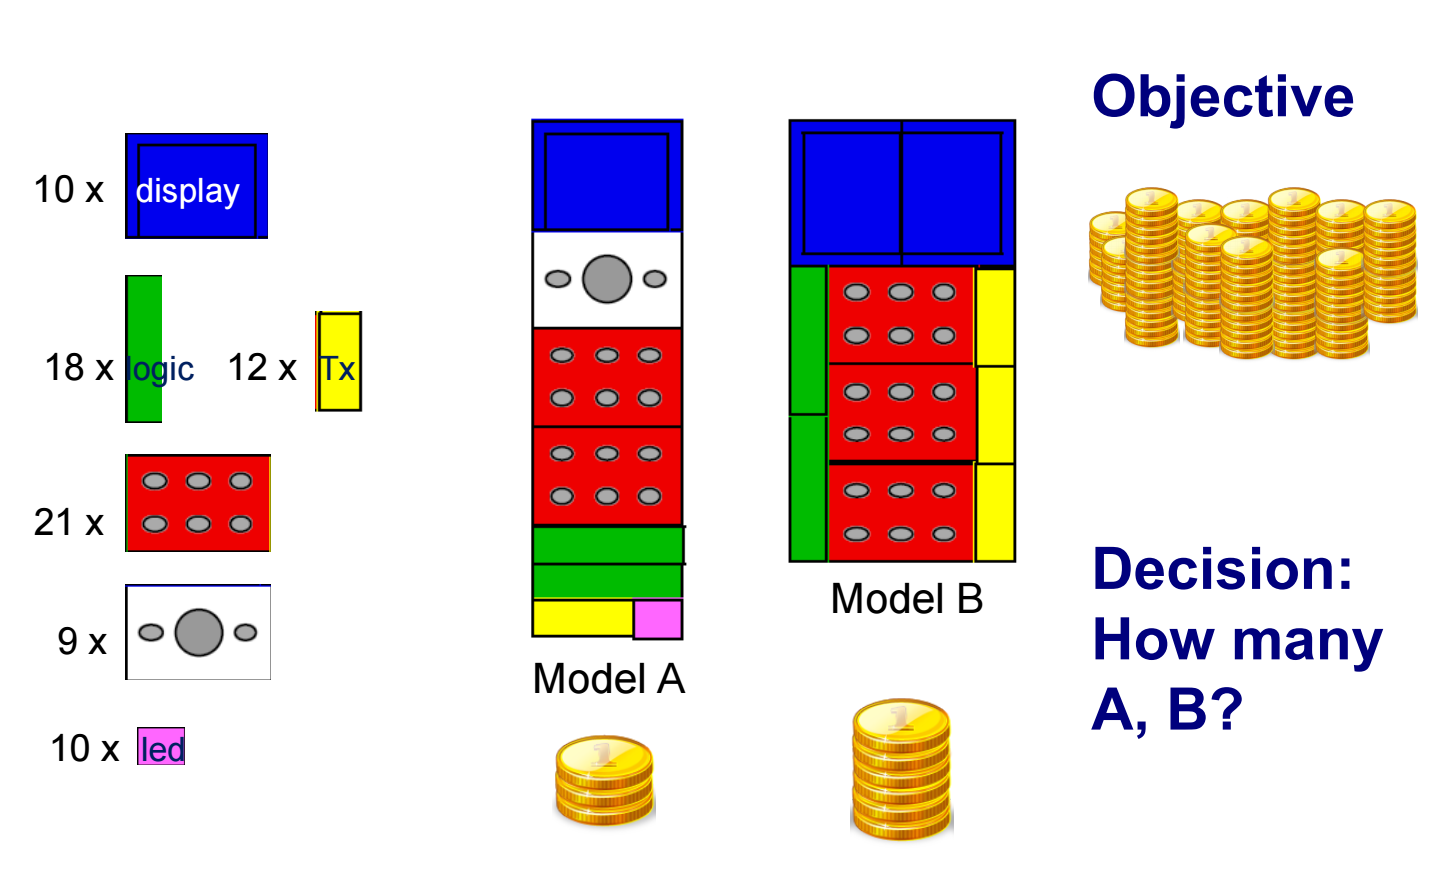
\includegraphics[width=0.7\textwidth]{images/l1-telefono.png}
\end{figure}

Per risolvere questo problema si possono usare varie strategie:

\begin{itemize}
	\item \textbf{Greedy}: scelgo di costruire il massimo numero di telefoni del modello con il prezzo più alto. Però non ho la garanzia che la soluzione trovata sia ottima.
	\item \textbf{Local search}: determino un certo numero di telefoni da produrre in modo da trovare una possibile soluzione sub-ottima per poi andare a modificare il numero di telefoni prodotti, cercando di migliorare il guadagno. Anche in questo caso non ho la garanzia che la soluzione trovata sia ottima.
	\item \textbf{Global search}: provo tutte le possibili combinazioni di telefoni che posso produrre, così facendo sono sicuro di trovare una soluzione ottima.
\end{itemize}


Un altro possibile problema è quello del contadino che possiede 12 ettari di terra dove può coltivare patate o pomodori, avendo a disposizione 70kg di semi di pomodoro, 18 tonnellate di tuberi di patate e 160 tonnellate di fertilizzante. Il contadino sa che un ettaro di campo coltivato a pomodori produce un guadagno di 3000 euro mentre uno di patate 5000. Per coltivare un ettaro a pomodori servono 7kg di semi e 10 tonnellate di fertilizzante, mentre un ettaro di patate richiede 3 tonnellate di tuberi e 20 di fertilizzante.

Questo problema è simile a quello del telefono, con la differenza che in questo caso gli ettari possono essere frazionati e quindi l'approccio combinatorio non può essere utilizzato.

L'idea è quindi quella di formulare un modello che descrive la soluzione ottima, anziché formulare un algoritmo che lo risolve.

Come prima cosa è necessario identificare le \textbf{variabili decisionali}, in questo caso $x_T$ e $x_P$ che rappresentano gli ettari coltivati. 
Poi si deve definire la \textbf{funzione obiettivo} che si vuole ottimizzare, in questo caso $\max 3000 x_T + 5000 x_P$.
Infine è necessario definire i \textbf{vincoli del problema} per modellare il consumo di risorse. In questo caso:

\begin{align*}
	x_T + x_P &\leq 12 \text{ vincolo sulla terra} \\
	7 x_T &\leq 70   \text{ vincolo sui semi di pomodoro} \\
	3 x_P &\leq 18 \text{ vincolo sui tuberi} \\
	10 x_T + 20 x_P &\leq 160 \text{ vincolo sul fertilizzante} 
\end{align*}

Con questa formulazione del problema non dico niente riguardo la soluzione del problema, ma posso utilizzare il modello creato per trovarla utilizzando dei metodi matematici dato che l'insieme di vincoli può essere visto come un sistema di disequazioni.

Un primo approccio è quello di partire da un valore di partenza della funzione obiettivo, ad esempio 27000 e provare a migliorarlo utilizzando la discesa di gradiente, fino a trovare un punto del piano che corrisponde ad un valore ottimo.
Con questo approccio posso anche dire che la soluzione trovata è ottima, perché tutte le altre soluzioni migliori richiedono un maggior numero di risorse.

\begin{figure}[htbp]
	\centering
	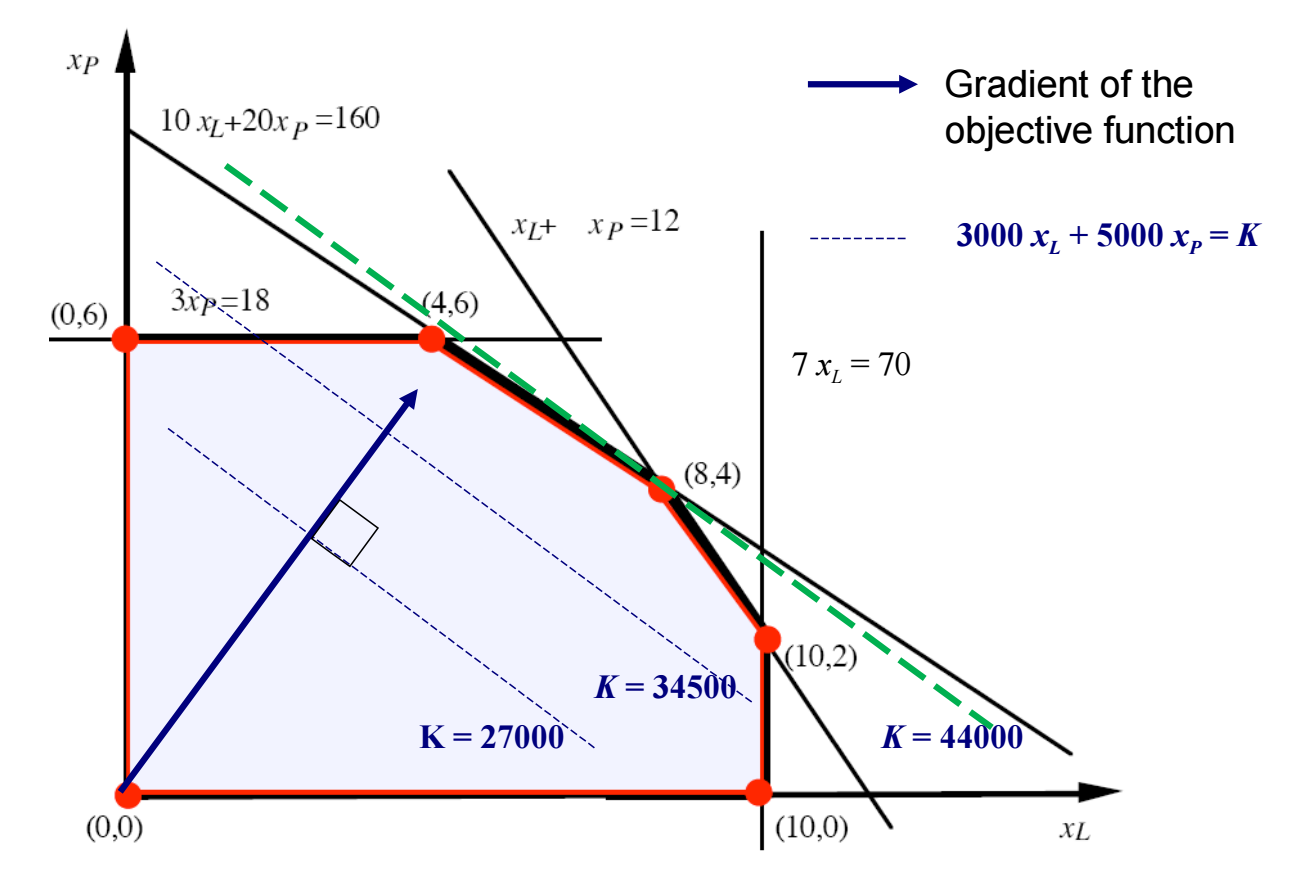
\includegraphics[width=0.5\textwidth]{images/l1-poligono.png}
\end{figure}


Tutto questo funziona perché sia i vincoli che la funzione obiettivo sono \textbf{lineari} e le variabili sono numeri reali. Questo tipo di modelli prende quindi il nome di \textbf{Linear Programming}.

Da notare che in questo caso la soluzione ottima è su un vertice intero, ma è un caso. Se le variabili utilizzate possono essere solo intere la situazione diventa più complessa perché è necessario effettuare delle approssimazioni.

\section{Approccio della ricerca operativa}

\begin{figure}[htbp]
	\centering
	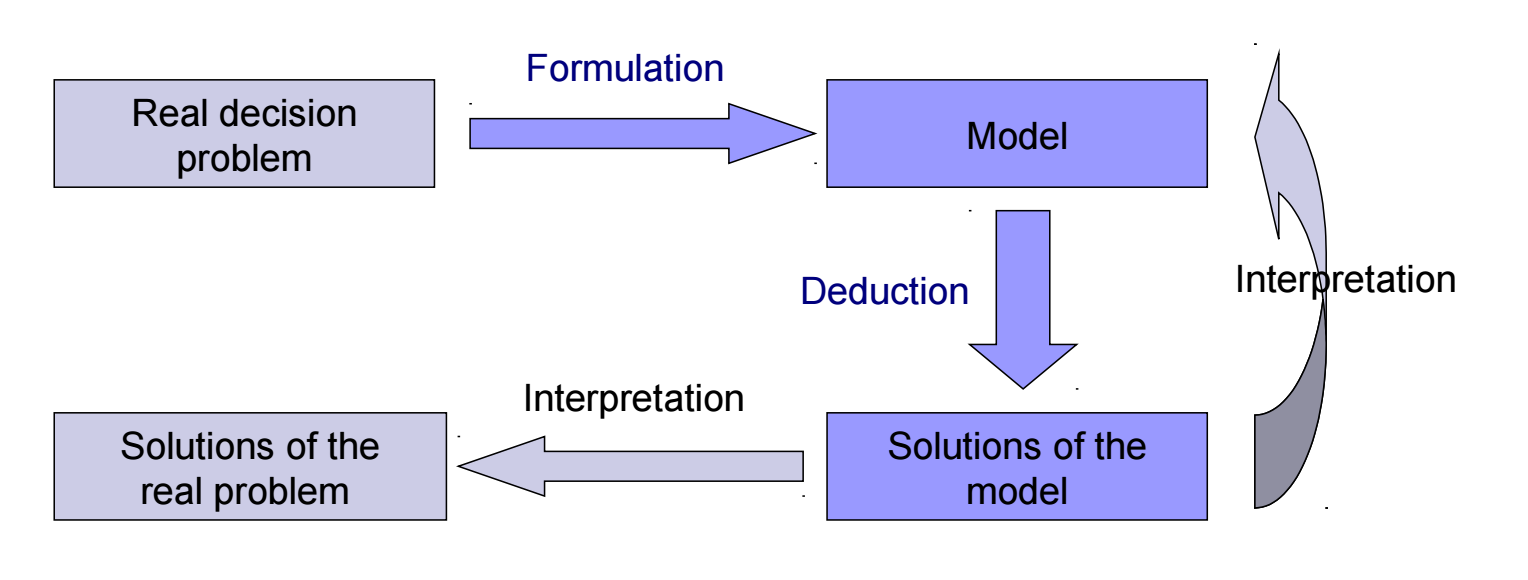
\includegraphics[width=0.7\textwidth]{images/l1-approccio.png}
\end{figure}

L'approccio precedentemente descritto è quello della ricerca operativa: si parte da un problema reale che viene formalizzato utilizzando un modello. Dal modello viene trovata una soluzione ottima per esso, la quale deve poi essere trasformata nella soluzione del problema reale.
Questo secondo passo può essere necessario perché nel modellare il problema può essere che sia stato necessario modificare alcuni vincoli, oppure utilizzare delle variabili reali anziché intere.

Si possono quindi definire due fasi: una di \textbf{formulazione} del modello e una di \textbf{deduzione} della soluzione, utilizzando alcuni algoritmi già definiti o personalizzati.

\section{Programma del corso}

\begin{enumerate}
	\item Ripasso e approfondimento delle tecniche di programmazione lineare e della dualità.
		\begin{itemize}
			\item Modelli LP, metodo del simplesso, teorema della dualità.
			\item Column generation technique per modelli LP grandi. Ovvero la creazione di modelli dinamici per evitare le limitazioni della memoria.
			\item Applicazioni: pianificazione della produzione, gestione del flusso di rete.
		\end{itemize}
	\item Metodi avanzati per la programmazione lineare intera mista (\textbf{MILP}).
		\begin{itemize}
			\item Formulazioni alternative, Branch \& Bound, Branch \& Cut.
			\item Applicazioni: Traveling Salesman Problem, localizzazione dei magazzini, set cover.
		\end{itemize}
	\item Meta euristiche per l'ottimizzazione combinatoria.
		\begin{itemize}
			\item Neighbourhood search e varianti.
			\item Algoritmi genetici.
		\end{itemize}
	\item Network optimization: modellazione dei problemi di ottimizzazione con i grafi. \textit{Potrebbe non essere affrontato.}
	\item \textbf{Laboratorio}:
		\begin{itemize}
			\item Online optimization server
			\item Optimization software and Algebraic modelling languages
			\item Optimization libraries (Cplex, Coin-OR, Scip)
		\end{itemize}
\end{enumerate}


\section{Informazioni pratiche}

Ci saranno dei laboratori nell'orario delle lezioni, verrà specificato nel sito quando ci saranno.

Non ci sono libri, vengono fornite le dispense dal professore e saranno in inglese.

Per ottenere il software che verrà utilizzato il laboratori è necessario registrarsi sul sito \url{http://www.math.unipd.it/userlist/subscribe/?idlist=277}, utilizzando la chiave \texttt{MeMoCO.16}. Per scaricare gratuitamente CPlex Optiumization Suite è necessario registrarsi alla IBM Academic Initiative.

L'esame è composto da:

\begin{itemize}
	\item Due esercitazioni di laboratorio, una sulla modellazione MILP e una sulle meta-euristiche, da consegnare qualche giorno prima dell'orale. Da fino a 10 punti.
	\item Esame orale che consiste nella discussione delle esercitazioni di laboratorio e delle domande teoriche sui contenuti del corso. Da fino a 20 punti. Forse si può fare in italiano.
	\item Progettino opzionale per ottenere un bonus da 2 a 6 punti. Il progetto riguarda la modellazione di un problema accordato con il docente e risolto utilizzando delle meta-euristiche o in modo esatto. Può essere fatto anche dopo lo scritto.
\end{itemize}



	% !TEX encoding = UTF-8
% !TEX program = pdflatex
% !TEX root = AALP.tex
% !TEX spellcheck = it-IT

% 6 Ottobre 2016

\chapter{Il mini linguaggio funzionale}

\section*{Testi di riferimento}

\begin{itemize}
	\item Types and Programming Languages (B. Pierce) 
	\item Practical Foundations for Programming Languages - Capitoli 1 e 2, consigliato leggerli prima della prossima lezione
\end{itemize}

\section{Teoria dei linguaggi di programmazione}

Si vuole descrivere il comportamento dei programmi in un modo preciso e formale, definendo una sintassi e una semantica.
Definire la sintassi è abbastanza semplice, la semantica è invece più complessa perché può avere varie sfumature:

\begin{itemize}
	\item \textbf{Semantica operazionale}: descrive come evolve la computazione del programma.
	\item \textbf{Semantica denotazionale}: descrive il programma in termini matematici, come una relazione tra l'input e l'output.
	\item \textbf{Semantica assiomatica}: descrive il programma utilizzando delle proprietà che sono vere per un certo programma, per poi utilizzarle per derivarne di nuove.
\end{itemize}

\noindent Noi ci concentreremo sulla semantica operazionale che viene verificata mediante tecniche di analisi statica sfruttando: sistemi di tipi, logiche temporali e interpretazione astratta.
Una volta fissato un sistema di tipi, questa verifica del programma può anche essere automatizzata.

\section{Linguaggi funzionali}

Studiare i tipi risulta più semplice sui linguaggi funzionali che su quelli imperativi.
Inoltre, lo stile di programmazione funzionale risulta più elegante perché è concentrato sul \textit{``what to do''} anziché \textit{``how to do''}.

\begin{lstlisting}[language=Java, caption=Confronto tra Java 5 e Java 8: nel secondo caso è subito chiaro l'intento del programmatore inoltre non vengono aggiunte variabili \textit{mutable}. Tuttavia l'esempio non usa le caratteristiche funzionali di Java8]
// Java 5
boolean found = false;
for(String city : cities){
	if (city.equals("Chicago")) {
		found=true;
		break;
	}
}
System.out.println("Found?" + found);
	
// Java 8
System.out.println("Found?" + cities.contains("Chicago"));
\end{lstlisting}

\begin{lstlisting}[language = Java, caption=Confronto tra Java 5 e Java 8: l'utlilizzo delle funzioni lambda rende il codice più conciso. Inoltre non vengono usate variabili mutabili e il codice è facilmente parallelizzabile.]
// Java 5
Collection<Person> people = ...;
int maxAge = -1;
for (Person p : people) {
	if (p.getGender() == MALE && p.getAge() > maxAge){
		maxAge = p.getAge();
	}
}

// Java 8
Collection<Person> people = ...;
final int maxAge = people.stream()
										      .filter(p -> p.getGender() == MALE)
										      .mapToInt(p -> p.getAge())
										      .max();
\end{lstlisting}

\noindent Tra le caratteristiche distintive dei linguaggi funzionali c'è l'\textbf{assenza degli assegnamenti}: ci sono delle variabili ma queste rappresentano dei valori e non delle aree di memoria modificabili. Vengono quindi solamente rappresentati dei valori immutabili.

Segue quindi che non ci sono side-effects: la chiamata di una funzione può essere sostituita con il suo risultato (\textbf{referential transparency}). Questo non è più valido se ad esempio la funzione stampa qualcosa a video e poi ritorna un risultato, pertanto se una funzione è pura, questa non può neanche produrre delle stampe a video.

Sembra una limitazione, ma in realtà così facendo si hanno vari vantaggi:
\begin{itemize}
	\item Il codice diventa più affidabile e più riusabile.
	\item Due funzioni che lavorano su dati diversi come \texttt{f(x)} e \texttt{g(y)} possono essere eseguite in parallelo senza problemi.
	\item Tutto ciò che entra ed esce dalla funzione può essere sottoposto a type check e quindi al compilatore basta solo il prototipo. Inoltre, se c'è un errore logico nella definizione della funzione è facile che questo si rifletta anche in un errore di tipo.
\end{itemize}

\noindent Un'altra caratteristica chiave è che le funzioni sono oggetti \textbf{first class}, ovvero sono a tutti gli effetti degli oggetti che possono essere passati come parametro ad altre funzioni. 
Le funzioni che prendono in input altre funzioni vengono chiamate funzioni \textbf{higher order}.
Ciò permette di scomporre un problema in sotto-problemi, utilizzare delle funzioni semplici per risolvere i sotto-problemi, per poi combinare le funzioni utilizzando delle funzioni higher-order.

\section{Sintassi del nostro linguaggi $\mathcal{L}$}

\begin{align*}
	x \in Var & &\\
	n \in Num & &\\
	Termini \: M, N &::= x &\text{ variabili} \\
								&|\: n \:|\: \text{true} \:|\: \text{false} &\text{ costanti intere e booleane} \\
								&|\: M + M \:|\: M - M &\text{ operazioni intere} \\
								&|\: \text{if} \: M \: \text{then} \: M \: \text{else} \: M &\text{ condizionale} \\
								&|\: \text{fn } x.M &\text{ dichiarazione di una funzione} \\
								&|\: M \: M &\text{ applicazione di una funzione}
\end{align*}

\noindent Un programma è quindi un termine chiuso \textit{M}, ovvero che non ha variabili libere e l'esecuzione del programma equivale a trovare il valore del termine \textit{M}.

Alcuni esempi di programmi:

\begin{align*}
3 + 2 &\\
\text{fn} \:  x.x &\:\text{// funzione identità} \\
\text{fn} \: x.3 &\: \text{// funzione costante 3} \\
\text{fn} \: x.x+1 &\: \text{// funzione successore} \\
\text{fn} \: x.x+1 \: 3 &\: \text{// funzione successore applicata al numero 3} \\
\text{fn} \: x.\text{fn} \: y . x+y &\: \text{// funzione somma con due argomenti (currificata)} \\
\text{fn} \: x. (\text{fn} \: y . x+y   + 2) &\: \text{// funzione che ritorna la funzione $2+x$} \\
\underbrace{\text{fn} \: x.\text{fn}\ y.(x\: y)}_{M} &\: \text{// funzione che applica un'altra funzione} \\
(M \: \text{fn} \: z.z) \: 5 &\: \text{// applicazione della funzione identità al numero 5} \\
\text{if} \: 2 \: \text{then} \: \text{fn}\: x.x+x \: \text{else} \: 0 &\: \text{// utilizzo del condizionale, è sinteticamente corretto ma non a livello di tipi}
\end{align*}

\noindent Il comportamento dei programmi dipende poi dalla semantica che viene attribuita alle istruzioni.

\subsection{Variabili libere}

C'è poi il concetto di variabile \textbf{libera} o \textbf{legata}.
La variabile $x$ nel termine $\text{fn } x.x$ è legata, perché viene dichiarata dal termine, infatti $\text{fn}$ è un \textit{binder}.

Nel termine $x+y$ le due variabili sono libere, perché non si riesce ad attribuirgli un valore. Per funzionare un programma non deve avere variabili libere.
Mentre nel termine $\text{fn }y. x\: y$ la variabile $x$ è libera mentre la $y$ è legata. Si ottiene così una \textbf{clojure}, ovvero una funzione che per essere calcolata deve ricevere dei valori per le variabili libere.

Ci sono poi le funzioni \textbf{alpha-equivalenti}, ovvero funzioni che calcolano la stessa cosa, ma che utilizzano variabili legate con nomi diversi. Es: $\text{fn }y.y+1$ e $\text{fn }x.x+1$.

Più formalmente si possono definire le variabili libere in modo induttivo.
Dato un termine $M$, le variabili libere di $M$ vengono indicate con $fv(M)$ e sono definite induttivamente come:

\begin{align*}
	fv(x) &= \{ x \} \\
	fv(n) =fv(\text{true}) = fv(\text{false}) &= \emptyset \\
	fv(M + N) = fv(M-N) &= fv(M) \cup fv(N) \\
	fv(\text{if } M_1 \text{ then } M_2 \text{ else }M_3) &= fv(M_1) \cup fv(M_2) \cup fv(M_3) \\
	fv(\text{fn }x.M) &= fv(M) \setminus \{x\} \\
	fv(M \: N) &= fv(M) \cup fv(N)
\end{align*}

\noindent Un termine senza variabili libere viene detto \textbf{chiuso} e i programmi sono definiti da dei termini chiusi.

\subsection{Sostituzione}

Definiamo ora l’operazione di sostituzione di una variabile con un termine, necessaria per la definizione della semantica del linguaggio. 
Indichiamo con $M \{x := N\}$ il termine $M$ in cui la variabile $x$ è stata sostituita con il termine $N$.
Nel seguito useremo una notazione compatta in cui \textit{c} varia nell’insieme delle costanti intere e booleane, mentre $op(M_i)_{i\in I}$ varia nell’insieme delle operazioni aritmetiche e booleane.

\begin{align*}
	x \{x := N\} &= N \\
	y \{x := N\} &= y \\
	c \{x := N\} &= c \\
	op(M_i)_{i \in I}\{x := N\}  &= op(M_i\{x := N\} )_{i \in I} \\
	(M_1 + M_2) \{ x:= N \} &= M_1\{x := N\} + M_2 \{x := N\} \\
	(\text{fn} \: x.M)\{x := N\} &= \text{fn }x.M \\
	(\text{fn} \: y.M)\{x := N\}  &= \text{fn }y.M\{x := N\} \text{ if } y \notin fv(N) \\
	(M_1 \: M_2) \{x := N\}  &= (M_1\{x := N\} \: M_2 \{x := N\} )
\end{align*}

\noindent Quando applico una sostituzione $M\{x := N\}$ devo stare atteno a sostituire solamente le occorrenze libere di $x$ ed è inoltre importante che i termini che vado ad aggiungere non vengano catturati da un altro binder.
Per evitare questo problema è necessario rinominare le variabili problematiche per alpha conversione.

Ad esempio $(\text{fn }x.x)\{x := 3\}$ \textbf{non} è $\text{fn }x.3 $ ma $\text{fn }x.x$ e allo stesso modo $(\text{fn }y.x+y)\{x := y\}$ \textbf{non} è $\text{fn }y.y+y$ ma $(\text{fn }x.x+z)\{x := y\} = \text{fn }z.y+z$.






	% !TEX encoding = UTF-8
% !TEX program = pdflatex
% !TEX root = InformationRetrieval.tex
% !TEX spellcheck = it-IT

% 6 Ottobre 2016

%\chapter{Rappresentazione dei documenti}
%\section{Analisi automatica del testo}

Tutto è iniziato quando George K. \textbf{Zipf}, uno studioso americano di linguistica ha formulato delle leggi empiriche che mettono in relazione la \textbf{frequenza di una parola} con la sua \textbf{forma} e \textbf{significato}. 
Solo in un secondo momento queste leggi sono state applicate all'indicizzazione dei documenti.

L'osservazione di partenza è stata quella che ci sono poche parole che sono veramente molto frequenti, come gli articoli, e che sono poco significative rispetto il contenuto informativo del documento. Ci sono poi tante parole poco frequenti, alcune delle quali sono fortemente correlate al contenuto informativo del documento. Il gioco è quindi quello di sfruttare al meglio tali parole.

Questo andamento può essere rappresentato graficamente, prima andando a contare le frequenze delle singole parole, per poi andare ad ordinarle da quella più frequente a quella meno frequente. La distribuzione così ottenuta è intera, ma può essere approssimata da un'iperbole.

Tipicamente in inglese:
\begin{itemize}
	\item Le due parole più frequenti sono \textit{the} e \textit{of}, mediamente sono il 10\% delle parole del documento.
	\item Le 6 parole più frequenti corrispondo a circa il 20\% delle occorrenze e le 50 parole più frequenti corrispondo a circa il 40\% dei testi. Questo deriva dal fatto che la lingua deve essere ridondante in modo che sia facile da capire.
	\item Considerando un'insieme di documenti molto ampio, circa la metà delle singole parole di quel campione compare una sola volta. Queste sono parole più significative dal punto di vista dell'informazione. Tuttavia è necessario tenere conto che in questo insieme di parole possono comparire anche gli errori di battitura.
\end{itemize}

\subsection{Legge di Zipf}

La legge di Zipf afferma che dato un campione di testi e calcolata la frequenza $f$ delle parole, una volta che si sono messe le parole in ordine decrescente di frequenza, cioè si sono ordinate le parole in base al ragno \textit{r}, la distribuzione che si ottiene ha un andamento assimilabile ad una iperbole e si ha che

$$
r \times f = k
$$

ovvero la distribuzione è data da $ f = \cfrac{k}{r}$.

Se anziché ragionare in termini di frequenza assoluta si passa a considerare quella relativa, ovvero la probabilità osservata di occorrenza della parola, la legge di Zipf può essere riscritta come 

$$
r \times P_r = c
$$

Dove $P_r$ è la probabilità di occorrenza della parola che occupa il rango $r$-esimo e $c$ è una costante ($c = 0.1$ per l'inglese).

Si ha che per la lingua inglese $c \approx 0,1$ e l'iperbole che si ottiene è riportata in figura \ref{fig:zipf}

\begin{figure}[htbp]
\centering
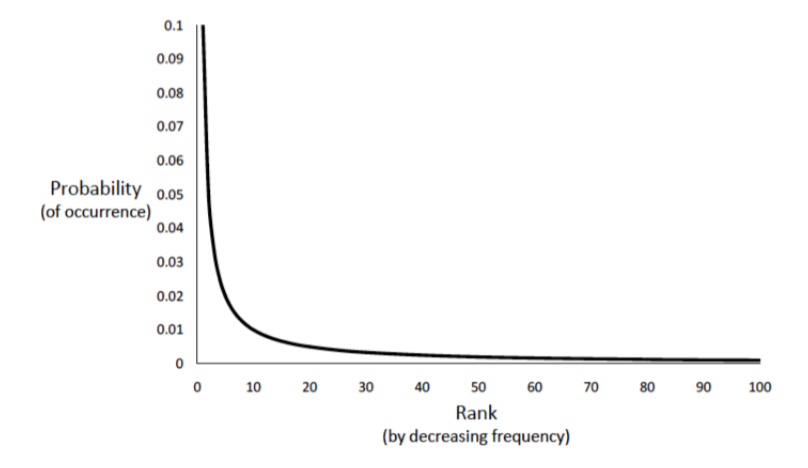
\includegraphics[width=0.55\linewidth]{images/l3-zipf}
\caption{Rango rispetto la probabilità di occorrenza assumendo valida la legge di Zipf con $c = 0.1$}\label{fig:zipf}
\end{figure}

\subsection{Indicazioni di H.P. Luhn}

L'idea per l'indicizzazione è quindi quella di definire due soglie di \textit{cut-off} per evitare di prendere in considerazione le parole troppo frequenti, perché poco significative, e quelle troppo poco, per limitare l'effetto degli errori di battitura.

Ogni parola ha un certo \textbf{resolving power}, ovvero una certa capacità di discriminare il contenuto del documento da quello degli altri e di caratterizzare il contenuto della collezione.

\begin{figure}[htbp]
	\centering
	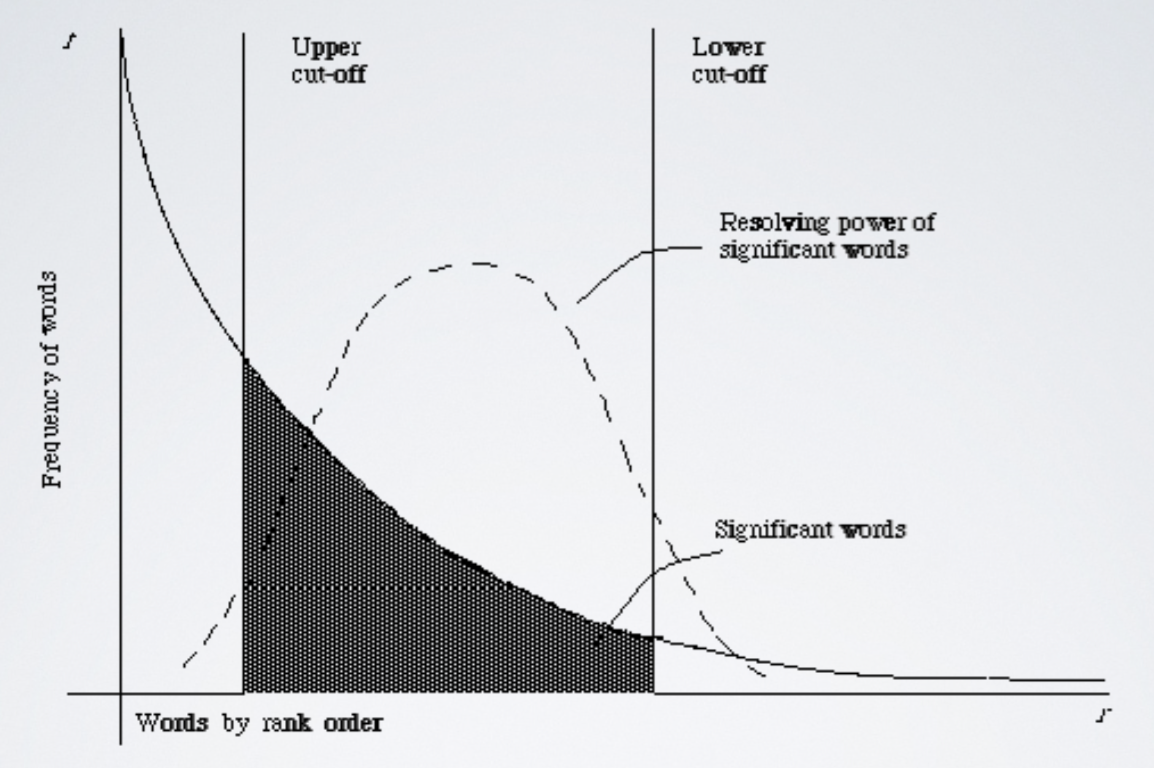
\includegraphics[width=0.55\linewidth]{images/l3-cutoff}
	\caption{Plot della curva $r \times f$ che evidenzia la posizione delle parole significative.}
\end{figure}

Questo vale per le collezioni generiche dei documenti, mentre se si parla di un argomento specifico si può dare maggiore peso a determinate parole. Ad esempio può capitare che se viene preso in esame un manuale di MySQL è ovvio che le parole ``MySQL'' e  ``table'' compariranno tante volte anche se non sono articoli.

C'è anche un altro discorso relativo alla forma plurale delle parole, che in conteggio di frequenza viene considerata come una parola diversa, quando in realtà può essere che abbia lo stesso valore informativo della forma singolare. In alcuni casi è quindi opportuno sommare le occorrenze della forma plurale e di quella singolare.

Si ha quindi che i passi per applicare le indicazioni di Luhn sono:

\begin{itemize}
	\item Si calcoli la frequenza di ogni descrittore in ogni documento della collezione di riferimento. C'è inoltre da scegliere come trattare le parti di contorno dei documenti come l'indice, la premessa, ecc. tali parti tipicamente non vengono considerate.
	\item Si calcoli la frequenza totale di ogni descrittore.
	\item Si ordino i descrittori per frequenza decrescente.
	\item Si scelga una soglia di \textit{upper cut-off} e si rimuovano dalla lista i descrittori con frequenza superiore alla soglia. In questo modo si rimuovono gli articoli, le preposizioni, ecc.
	\item Si scelga un'altra soglia di \textit{lower cut-off} e si rimuovano dalla lista i descrittori con frequenza inferiore al valore di soglia. In questo modo si rimuovono i descrittori ``rumore''  o che non apportano alcun contribuito alla descrizione del contenuto.
\end{itemize}

\noindent Entrambe le soglie possono essere calcolate in modo euristico.

Le parole che vengo eliminate dalle soglie di cut-off vengono nominate \textbf{stop word} e sono raccolte nella lista che prende il nome di \textbf{stop list}.


\textbf{{\color{Red} Possibile esercizio:}} Domande relative alle osservazioni proposte da Zipf e Luhn.

\section{Indicizzazione}

L'indicizzazione ha l'obiettivo di rappresentare il contenuto informativo di un documento e nel tempo questo processo ha preso una struttura a fasi.
Il documento viene rappresentato da dei descrittori che vengono utilizzati per la costruzione degli indici utili al reperimento dell'informazione.

Quindi l'indicizzazione fornisce automaticamente una rappresentazione più compatta e direttamente utilizzabile del contenuto informativo del documento. Gli indici sono utilizzati come surrogati del contenuto del documento durante la fase di reperimento.

L'indicizzazione può essere svolta:
\begin{itemize}
	\item manualmente
	\item in modo automatico
	\item in modo semi-automatico, quando è necessario intervenire all'interno del processo per prendere delle decisioni che non possono essere prese in modo automatico.
\end{itemize}

\noindent Tutti questi metodi funzionano estraendo direttamente dal documento le informazioni. Tuttavia possono essere estesi in modo che vengano presi in considerazione anche dei dizionari o delle meta-informazioni.

\begin{figure}[htbp]
	\centering
	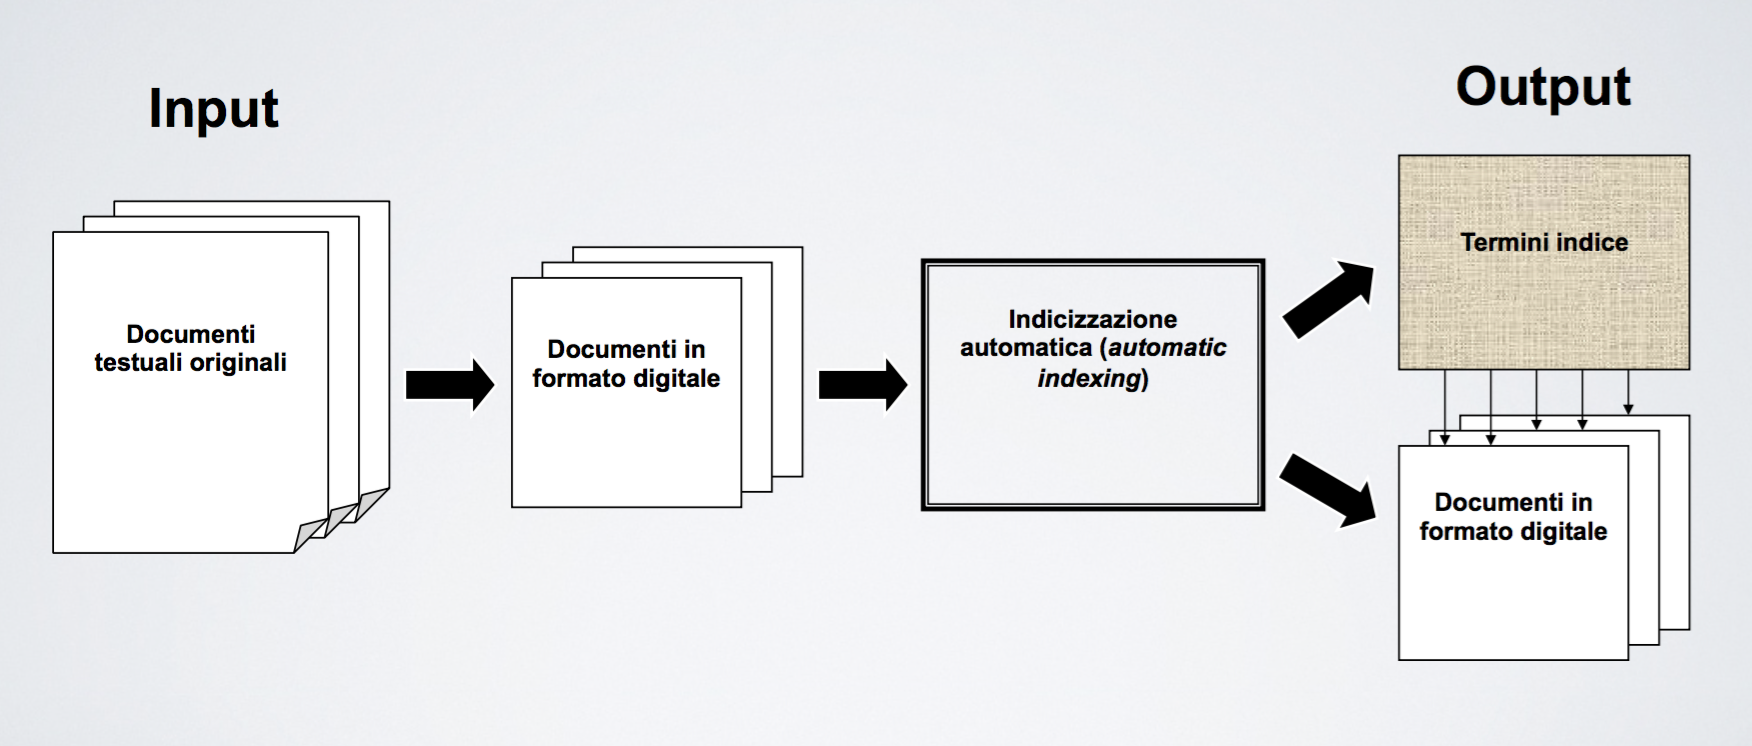
\includegraphics[width=0.7\linewidth]{images/l3-indicizzazione}
	\caption{Schema generale dell'indicizzazione}
\end{figure}

\subsection{Indicizzazione automatica dei testi}

L'indicizzazione automatica di un documento testuale è un processo che esamina automaticamente gli oggetti informativi (parole, frasi, didascalie, figure, ecc.) che compongono il documento e produce una lista di termini indice presenti nell'intera collezione dei documenti.

L'estrazione dei termini indice viene fatta da appositi algoritmi e, una volta estratti, questi vengono collegati ai diversi documenti che li contengono.
Così facendo durante il reperimento sarà sufficiente fare riferimento ai termini indice e non all'intera collezione.

\subsection{Attuazione dell'indicizzazione automatica}

L'indicizzazione automatica dei documenti testuali viene eseguita in più fasi, che devono essere attuate in sequenza:

\begin{enumerate}
	\item Analisi lessicale e selezione delle parole.
	\item Eventuale rimozione delle stop word.
	\item Riduzione delle parole originali alle rispettive radici (\textit{STEM}). Ad esempio le forme plurali vengono ridotte a quelle singolari.
	\item Composizione dei termini. Come ad esempio ``information retrieval''. Ovvero le parole vengono combinate tra loro quando si trovano ad una determinata distanza.
	\item Creazione dell'indice.
	\item Eventuale pesatura degli elementi dell'indice. 
\end{enumerate}

Alla fine di queste fasi l'indice sarà composto da parole, termini e frasi che noi riteniamo significative, assieme alle informazioni del peso che gli diamo e alla loro frequenza all'interno dei documenti.









	\chapter{Laboratorio}

\section{Un po' di cose su R}\label{un-po-di-cose-su-r}

\begin{itemize}
\item
  Tutti gli oggetti sono vettori
\item
  \texttt{ls()} per vedere le variabili disponibili
\item
  \texttt{x\ \textless{}-\ c(2,3,4,5)} crea un vettore con 1,2,3,4.
\item
  notazione \texttt{{[}1:20{]}} per un vettore con la successione da 1 a
  20
\item
  \texttt{xx\ \textless{}-\ seq(from=100,\ to=1)} crea sempre una
  sequenza di numeri, con parametro opzionale \texttt{by} per
  specificare lo step
\item
  \texttt{rep(2,5)} crea un vettore con 5 elementi uguali a 2
\item
  \texttt{a\ \textless{}-\ c(rep(2,3),4,5,rep(1,5))},
  \texttt{a\ =\ 2\ 2\ 2\ 4\ 5\ 1\ 1\ 1\ 1\ 1}
\item
  \texttt{2*x} esegue il prodotto scalare
\item
  \texttt{length(x)} per la lunghezza del vettore
\item
  \texttt{max(x)} e \texttt{min(x)}
\item
  \texttt{sum(x)} che ritorna un vettore di un solo elemento con la
  somma
\item
  \texttt{mean(x)}, \texttt{var(x)}, \texttt{range(x)}
\item
  \texttt{x{[}7{]}} per estrarre il settimo elemento di \texttt{x},
  l'indice credo parta da 1
\item
  \texttt{x{[}-4{]}} ritorna un vettore senza il quarto elemento
\item
  \texttt{x\ \textless{}-\ matrix(c(2,3,5,7,11,13),nrow\ =\ 3)} crea una
  matrice con gli elementi specificati e 3 righe. Alternativamente è
  possibile specificare anche il numero di colonne.
\item
  \texttt{x2\ \textless{}-\ scan("nome\ file",\ sep="")} con
  \texttt{sep} opzionale, per caricare il contenuto di un file in un
  vettore, per caricare una matrice
  \texttt{x2\ \textless{}-\ matrix(scan(...),\ ncol\ =\ 3,\ byrow=TRUE}.
\item
  \texttt{str(x)} specifica la struttura dell'oggetto
\item
  \texttt{dim(x)} ritorna la dimensione di una matrice, se invocato con
  un vettore ritorna \texttt{NULL}.
\item
  \texttt{x{[}18,{]}} per ottenere la 18-esima riga di una matrice
\item
  \textbf{Dataframe}: matrice le cui colonne possono avere formati
  diversi
\item
  \texttt{ciliegi\ \textless{}-\ read.table("nome\ file")}.
\item
  \texttt{names(ciliegi)} è il vettore con i nomi delle colonne del
  dataframe
\item
  \texttt{names(ciliegi)\ \textless{}-\ c("diametro",\ "altezza",\ "volume")}
  permette di impostare il nome delle colonne, può anche essere
  specificato come parametro opzionale \texttt{col.names} della
  funzione \texttt{read.table}.
\item
  \texttt{summary(ciliegi)} fornisce degli indicatori per ciascuna
  colonna
\item
  \textbf{Mediana}: elemento centrale di una distribuzione ordinata in
  senso crescente, \textbf{primo e terzo quartile}: generalizzazione
  della mediana, rispettivamente l'elemento che sta al 25 e 75 per cento
  della distribuzione. La differenza tra i due quartili da l'idea di
  quanto è variabile la distribuzione.
\item
  I dataframe possono essere acceduti anche con il nome della colonna
  \texttt{ciliegi\$volume}.
\item
  \textbf{attach di un file}: aggiungere al workspace un oggetto, ovvero
  \texttt{attach(ciliegi)} permette di accedere al nome della colonna
  direttamente utilizzando \texttt{volume}. Come complementare c'è il
  comando \texttt{detach}.
\item
  \texttt{hist(diametro)} crea l'istogramma per il diametro
\item
  \texttt{help(hist)} per avere l'help di una funzione
\item
  l'istrogramma che viene generato di default può contenere dei buchi,
  conviene quindi adattare il numero di colonne utilizzando il parametro
  \texttt{breaks}
\item
  \texttt{boxplot(diametro)} fornisce il box plot di un valore, è un
  grafico che rappresenta la mediana, i quartili e il 5 e 95\%. Risulta
  più espressivo dell'istogramma. L'ampiezza della scatola rappresenta
  la variabilità dei dati.
\item
  \texttt{ciliegi{[}altezza\textgreater{}80,{]}} prende tutti i ciliegi
  con altezza maggiore di 80.
\item
  \texttt{library(MASS)} permette di caricare la libreria MASS
\item
  \texttt{search()} permette di visualizzare la lista degli ottetti in
  cui R va a cercare quando deve eseguire un comando
\item
  Gli attributi qualitativi vengono trattati come tipo Factor
\item
  \texttt{table(painters\$School)} crea la tabella con le frequenze
  delle varie qualità
\item
  \texttt{barplot(..)} fa il plot delle barre per una variabile discreta
\item
  \texttt{pie(...)} fa il grafico a torta, anche se è sconsigliabile
  utilizzare un grafico a torta perché per l'occhio umano fa fatica a
  vedere la differenza tra gli angoli.
\item
  come scale colori si possono utilizzare \texttt{heat.colors(k)},
  \texttt{rainbow(k)}, \ldots{}
\item
  \texttt{plot(x,y)} disegna un diagramma di dispersione, il parametro
  \texttt{pch} specifica il tipo di carattere, \texttt{pch=16}
  rappresenta i pallini pieni, \texttt{col} specifica il colore da
  utilizzare, possono indicare \texttt{col=painter\$School} per far
  variare il colore in base al valore dell'attributo quantitativo
\end{itemize}

	% !TEX encoding = UTF-8
% !TEX TS-program = pdflatex
% !TEX root = ../apprendimento_automatico.tex
% !TEX spellcheck = it-IT
\section{Lezione 5 - VC-Dimension e VC-Confidence}\label{lezione-5-vc-dimension-e-vc-confidence}

\subsection{Esempi di spazi delle ipotesi}\label{esempi-di-spazi-delle-ipotesi}

Seguono alcuni esempi di spazi per le ipotesi nei problemi di
apprendimento supervisionato, cioè quei problemi in cui si vuole
stabilire se un elemento \emph{x} appartiene o meno ad una classe.

\subsubsection{Iperpiani in R2}\label{iperpiani-in-r2}

\textbf{Iperpiano}: dato uno spazio a \emph{n}-dimensioni, un iperpiano
per quello spazio è un sottospazio di dimensione \emph{n-1}. Ad esempio gli
iperpiani in $R^2$ sono tutte le rette del piano.

Lavorando in $R^2$ lo spazio delle istanze è definito come:

$$
X = \{x | x \in R^2\}.
$$

Mentre lo spazio delle ipotesi è dato dalle dicotomie indotte da iperpiani in $R^2$, cioè da tutte le possibili divisioni del piano.

$$
H = \{f_{(w,b)}(x) | f_{(w,b)}(x) = sign(w \times x + b), w \in R^2, b \in R\}
$$

Così facendo vengono prese in considerazione tutte le rette che dividono
$R^2$ in due parti in modo che da una parte l'ipotesi valga 1 e dall'altra
-1.

\subsubsection{Dischi in $R^2$}\label{dischi-in-r2}

Sempre in $R^2$ è possibile considerare come spazio delle ipotesi tutte le
dicotomie indotte da dischi in $R^2$ e centrati nell'origine.

$$
H = \{f_b(x) | f_b(x) = sign(||x||^2 - b), w \in R^2, b \in R\}
$$

Il che vuol dire che all'interno del disco le ipotesi valgono -1 mentre
al di fuori valgono 1.

\subsubsection{\texorpdfstring{Congiunzione di \emph{m} letterali positivi}{Congiunzione di m letterali positivi}}\label{congiunzione-di-m-letterali-positivi}

Lo spazio delle istanze questa volta è dato da tutte le stringhe di \emph{m} bits

$$
X = \{s | s \in \{0,1\}^m\}
$$

Lo spazio delle ipotesi è dato da tutte le sentenze logiche che
riguardano i letterali positivi $l_1$,$l_2$,\ldots{},$l_m$ ($l_i$ è vero se
l'\emph{i}-esimo bit è 1) e che contengono solo l'operatore $\wedge$.

$$
H = \{ f_{(i_1,\ldots,i_j}(s) | f_{(i_1,\ldots,i_j}(s) \text{ equivale a } l_{i_1} \wedge l_{i_2} \wedge \ldots \wedge l_{i_j}, \{i_1\ldots{}i_j\} \text{ sottoinsieme di }  \{1..m\}\}
$$

\subsection{Misurare la complessità dello spazio delle ipotesi}\label{misurare-la-complessituxe0-dello-spazio-delle-ipotesi}

Considerato un determinato spazio delle ipotesi \emph{H}, questo
contiene sempre:

\begin{itemize}
\item
  L'\textbf{ipotesi più specifica}: ipotesi più stretta e consistente con
  i dati, nell'esempio del disco è il disco più stretto in grado di
  contenere tutti i punti negativi.
\item
  L'\textbf{ipotesi più generale}: quella più grande e consistente con i
  dati, sempre nell'esempio del disco, è quello più grande
  possibile che non contiene punti positivi.
\end{itemize}

\textbf{Shattering}: (frammentazione), dato \emph{S} sottoinsieme dello
spazio delle istanze, si dice che \emph{S} è frammentato dallo spazio
delle ipotesi \emph{H} se:

$$ 
\forall S' \in S, \exists h \in H, \text{ tale che } \forall x \in S, h(x) = 1 \text{ se e solo se } x \in S'.
$$

Cioè \emph{H} realizza tutte le possibili dicotomie di \emph{S}.

\emph{H} frammenta un certo insieme \emph{S} se è possibile trovare un
iperpiano \emph{h} che raccoglie tutti i punti dell'insieme \emph{S}. Ovvero per
tutte le dicotomie di \emph{S} esiste un iperpiano che riesce a
realizzarle.

\subsubsection{VC (Vapnik-Chervonenkis) Dimension}\label{vc-vapnik-chervonenkis-dimension}

La VC-Dimension è la dimensione di uno spazio delle ipotesi \emph{H}
definito su uno spazio delle istanze \emph{X} ed è data dalla
cardinalità del sottoinsieme più grande frammentato da \emph{H}.

$$
VC(H) =
\begin{cases}
max_{S \subseteq X} |S|&\text{ tale che \emph{H} frammenta } S  \\
 \infty& \text{ se S non è limitato}
\end{cases}
$$


Ad esempio se nello spazio delle ipotesi dato dagli iperpiani su $R^2$ ho 2 punti, lo spazio delle istanze viene frammentato da
\emph{H}, perché posso sempre trovare una retta che riesce a realizzare
tutte le possibili dicotomie di due punti su un piano.
Se nello spazio delle istanze ho 3 punti, riesco comunque a realizzare
tutte le dicotomie.
Se nello spazio delle istanze ho 4 punti qualsiasi non si riesce a
trovare un iperpiano che realizza la dicotomia, quindi \emph{VC(H) =
3}.

Segue che, prendendo uno spazio delle ipotesi di cardinalità finita si
ha che:

$$
VC(H) \leq log_2(|H|)
$$

Questo perché per ogni \emph{S} frammentato da \emph{H}, abbiamo
$|H| \geq 2^{|S|}$,
cioè per ogni dicotomia in \emph{S} esiste un ipotesi in \emph{H} che la
realizza, ovvero devono essere disponibili in \emph{H} tante ipotesi
quanti sono le dicotomie in \emph{H}.

Scegliendo un \emph{S} tale che $|S| = VC(H)$, si
ottiene $|H| \geq 2^{|S|}$, prendendo
il logaritmo si trova quello che si stava cercando, ovvero $VC(H) \leq log_2(|H|)$.

\textbf{Dal libro}:

Se un dataset contiene \emph{N} elementi, questi \emph{N} elementi
possono essere etichettati con degli 0 e 1 in $2^N$ modi diversi.

Se per ognuno di questi modi è possibile trovare un ipotesi $h \in H$
che separa tutte le istanze negative da quelle positive allora si dice
che \emph{H} frammenta il dataset \emph{N}. 
Il che vuol dire che il dataset \emph{N} può essere appreso con un errore empirico nullo.

Il massimo numero di punti che possono essere frammentati da \emph{H} è
detto \emph{VC(H)} e fornisce una misura della capacità di \emph{H}.

\subsection{Bound sull'errore di generalizzazione}\label{sec:vcc}

Considerando un problema di apprendimento binario, con:

\begin{align*}
\text{Training set }S &= \{(x_i,y_i), \ldots (x_N, y_N)\} \\
\text{Spazio delle ipotesi } H &=\{h_\theta(x)\} 
\end{align*}

Supponendo di avere un algoritmo di apprendimento \emph{L} che
restituisce l'ipotesi $h_{\theta*}$ che minimizza l'errore empirico su
\emph{S} espresso come $errore_S(h_\theta(x))$.

È possibile derivare un bound (limite superiore) per l'errore ideale o
errore di generalizzazione, valido con probabilità \emph{(1 - $\sigma$)} con
$\sigma$ piccolo a piacere:

$$
errore_D(h_\theta(x)) \leq  errore_S(h_{\theta}(x)) + g(N, VC(H), \sigma)
$$

Il primo termine $errore_S(h_{\theta}(x))$ dipende dall'ipotesi restituita
dall'algoritmo di apprendimento \textit{L}.

Il secondo termine $g(N, VC(H), \sigma)$ non dipende da \emph{L}, ma dal
numero di esempi di training utilizzati (inversamente proporzionale),
dalla \emph{VC-dimension} (direttamente proporzionale) e dalla
confidenza, ovvero dal termine $\sigma$.

Questo termine viene anche chiamato \textbf{VC-confidence} e risulta essere monotono rispetto al rapporto
$\frac{VC(H)}{N}$.

\textbf{Morale della favola}: la VC-Dimension sovrastima con confidenza $\sigma$ l'errore ideale.

\subsection{Structural Risk Minimization (SRM)}\label{sec:srm}

Approccio per la scelta dello spazio delle ipotesi proposto da Vapnik
che cerca di trovare un compromesso tra l'errore empirico e la
VC-Confidence.

Si considerano spazi delle ipotesi sempre più piccoli $H_1 \subseteq H2 \subseteq \ldots \subseteq H_n$ tali che $ VC(H_1) \leq VC(H_2) \leq \ldots \leq VC(H_n)$

Si seleziona lo spazio delle ipotesi $H_i$ che ha il valore del bound
sull'errore di generalizzazione più piccolo. ovvero la VC-Dimension minore.

\begin{figure}[htbp]
\centering
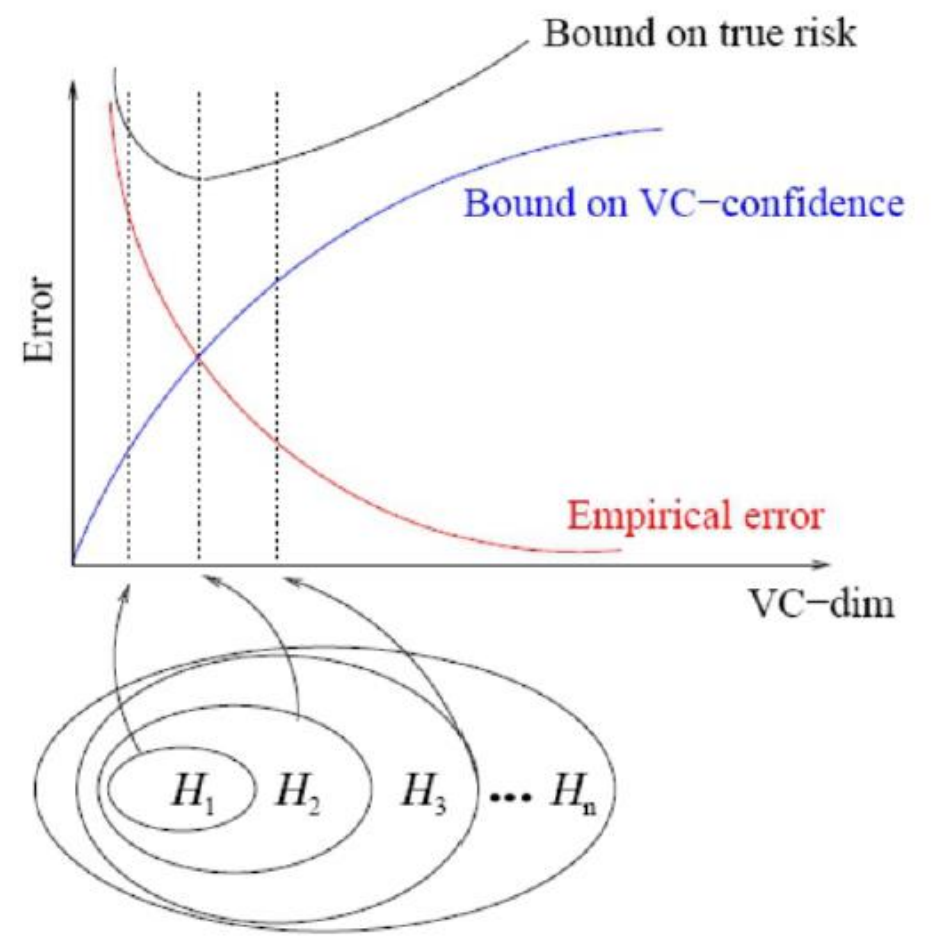
\includegraphics[width=0.5\textwidth]{./notes/immagini/l5-srm.png}
\caption{Structural Risk Minimization}
\end{figure}

	% !TEX encoding = UTF-8
% !TEX program = pdflatex
% !TEX root = AALP.tex
% !TEX spellcheck = it-IT

% 20 Ottobre 2016
% \section sistemi di tipi
% \subsubsection Teorema di Preservazione (Subject reduction)

% Dimostrazione del lemma di sostituzione (spostata al posto corretto in lezione5)

\subsubsection{Corollario di Subject-reduction}

\begin{center}
	Se $\emptyset \vdash M : T$ e $M \rightarrow^* M'$, allora $\emptyset \vdash M' : T$
\end{center}

\paragraph{Dimostrazione}

La dimostrazione viene fatta per induzione sul numero di passi che da $M$ portano ad $M'$.

Il caso base è quello con il cammino di lunghezza 0, ovvero quando $M = M'$ e la tesi è trivialmente vera.

Nel caso induttivo ho che $M \rightarrow^{*}_k M_1 \rightarrow M'$, pertanto per ipotesi induttiva ho che $\emptyset \vdash M_1 : T$. 

Ho poi che $M_1 \rightarrow M'$ e quindi posso applicare subject-reduction per ottenere che $\emptyset \vdash M' : T$.

\subsubsection{Teorema di Safety - Completo}

\begin{center}
	Se $\emptyset \vdash M : T $ e $M \rightarrow^* M'$ e $M' \not\rightarrow$, allora $M'$ è un valore.
\end{center}

\paragraph{Dimostrazione}

Alle due ipotesi posso applicare il corollario di subject-reduction, ottenendo che $\emptyset \vdash M' : T$.

Per il teorema di progressione ho poi che $M'$ è un valore oppure $M'$ fa un passo e va in $M''$, ma per ipotesi $M'$ non fa un passo e quindi $M'$ è per forza un valore.

\subsection{Esercizio sul typing}

Da notare che nel contesto iniziale non servono giudizi di tipo perché tutte le variabili che compaiono sono all'interno delle funzioni e che, non essendoci informazioni sui tipi, questi sono ignoti e pertanto è necessario fare anche inferenza durante la risoluzione dell'albero.

\begin{prooftree}	
	
	% App-1
	\AxiomC{$\checkmark$ $\textbf{\textit{T}} = \textbf{\textit{T}}_1 \rightarrow \textit{\textbf{T}}_3$}
	\LeftLabel{(\textsc{Var})}
	\UnaryInfC{$y : T, x : T' \vdash y : T_1 \rightarrow T_3$}
	
	% App-2
	\AxiomC{*}
	\LeftLabel{\textsc{(If)}}
	\UnaryInfC{$y : \textbf{\textit{T}}_1\rightarrow \textbf{\textit{T}}_3, x:T' \vdash \text{if true then }x \text{ else }y \: x : T_1$}
	\LeftLabel{\textsc{(App)}}
	\BinaryInfC{$y : T, x: T' \vdash y \: (\text{if true then }x \text{ else }y \: x) : \: T_3$}
	
	\LeftLabel{\textsc{(Fun)}}
	\UnaryInfC{$y : T \vdash \fn x : \textbf{\textit{T'}} . (y \: (\text{if true then }x \text{ else }y \: x)) : \textbf{\textit{T}}_2 = \textbf{\textit{T'}} \rightarrow \textbf{\textit{T}}_3$}
	
	\LeftLabel{\textsc{(Fun)}}
	\UnaryInfC{$\emptyset \vdash \fn y : \textbf{\textit{T}} . \fn x : T' . (y \: (\text{if true then }x \text{ else }x \: y)) : \textbf{\textit{T}} \rightarrow \textbf{\textit{T}}_2$} % T' \rightarrow ?
\end{prooftree}

\noindent Dal ramo sinistro di \textsc{(App)} riesco a chiudere con $T = T_1 \rightarrow T_3$ e quindi riporto l'informazione anche sul ramo destro.
La derivazione continua applicando \textsc{(IfThenElse)} e con $\Gamma = y:T_1 \rightarrow T_3, x:T'$:

\begin{prooftree}
	%if 1
	\AxiomC{$\checkmark$}
	\LeftLabel{\textsc{(True)}}
	\UnaryInfC{$\Gamma \vdash \true : \Bool$}
	
	%if 2
	\AxiomC{$\checkmark$  $\textbf{\textit{T}}_1 = \textbf{\textit{T'}}$}
	\LeftLabel{\textsc{(Var)}}
	\UnaryInfC{$y: T_1 \rightarrow T_3, x:T' \vdash x : T_1$}
	
	%if 3
	\AxiomC{**}
	\LeftLabel{\textsc{(App)}}
	\UnaryInfC{$y : \textbf{\textit{T'}} \rightarrow T_3, x:T' \vdash y \: x : \textbf{\textit{T'}}$}
	% per quello che ho scoperto 
	\UnaryInfC{$y : T_1 \rightarrow T_3, x:T' \vdash y \: x : T_1$}
	\LeftLabel{\textsc{(If)}}
	\TrinaryInfC{(*)$\Gamma \vdash \text{if true then }x \text{ else }y \: x : T_1$}
\end{prooftree}

\noindent Dal ramo centrale della regola \textsc{(IfThenElse)} scopro che $T_1 = T'$ e quindi aggiorno il ramo destro e il contesto, che ora è  $\Gamma = y:T' \rightarrow T_3, x:T'$.

\begin{prooftree}
	\AxiomC{$\checkmark$}
	\LeftLabel{\textsc{(Var)}}
	\UnaryInfC{$y:T' \rightarrow T_3 , x:T' \vdash y : T_4 \rightarrow T'$}
	
	\AxiomC{$\checkmark$}
	\LeftLabel{\textsc{(Var)}}
	\UnaryInfC{$y : T' \rightarrow T_3 , x :T'\vdash x : T_4$}
	
	\LeftLabel{\textsc{(App)}}
	\BinaryInfC{(**)$\Gamma \vdash y \: x : T'$}
\end{prooftree}

\noindent Da quest'ultimo albero trovo che $T' = T_4 = T_3$. Andando a sostituire il tutto trovo che:

\begin{itemize}
	\item $y : T' \rightarrow T'$
	\item $x : T'$
	\item $T_2 = T' \rightarrow T_3 = T' \rightarrow T'$
	\item $T = T_1 \rightarrow T_3 = T' \rightarrow T'$
	\item Il tipo del programma è quindi $(T' \rightarrow T') \rightarrow (T' \rightarrow T')$
\end{itemize}

\chapter{Estensioni del linguaggio funzionale}

\section{Unit}

Nei linguaggi funzionali, ogni funzione deve ritornare sempre un valore, tuttavia può capitare che delle funzioni non debbano ritornare un valore. In questo caso viene ritornato il tipo \text{Unit} che può assumere l'\textbf{unico} \textbf{valore} \texttt{()} o \text{unit}.

Ad esempio la funzione \texttt{print} in Scala ritorna un valore di questo tipo:

\begin{lstlisting}[language=Scala]
def print( x: Any) : Unit = {...}
\end{lstlisting}

\noindent allo stesso modo anche l'assegnamento in Scala ritorna un valore \text{Unit} mentre in C/C++ viene solitamente ritornato il valore assegnato (per concatenare le operazioni di assegnamento).

Aggiungere \text{Unit} al linguaggio vuol dire estendere la definizione:

\begin{align*}
	M &::= \ldots \: | \: \text{unit} \: | \: \ldots \\
	v &::= \ldots \: | \: \text{unit} \: | \: \ldots \\
	T &::= \ldots \: | \: \text{Unit} \: | \: \ldots 
\end{align*}

\noindent e allo stesso modo serve una regola di tipo:

\begin{prooftree}
	\AxiomC{}
	\LL{Unit}
	\UnaryInfC{$\Gamma \vdash \text{unit : Unit}$}
\end{prooftree}

\noindent La killer-feature del tipo \text{Unit} è la possibilità di implementare il call-by-name utilizzando il call-by-value.

Ad esempio, tornano alle nostre asserzioni in Scala

\begin{lstlisting}[language=Scala, caption=Version ``standard'' delle asserzioni]
var assEnabled = true
...
def assert(pred : Bool) = 
	if (assEnabled && !pred)
		throw Exc
...

assert(saldoConto() > 0)
\end{lstlisting}


\noindent possiamo utilizzare \text{Unit} per far funzionare il codice precedente come se fosse call-by-name ma senza specificarlo:

\begin{lstlisting}[language=Scala, caption=Version ``standard'' delle asserzioni]
var assEnabled = true
...
def assert(pred : Unit => Bool) = 
	if (assEnabled && pred() == false) /** l'invocazione con () passa Unit*/
		throw Exc
...
assert(fn x:Unit . (saldoConto() > 0) ) /** pseudo scala */
assert( () =>  (saldoConto() > 0) ) /** sintassi corretta (la funzione anonima non ha parametri) */
\end{lstlisting}

\noindent In questo caso con la sintassi call-by-value viene calcolato il valore del parametro, ma in questo caso il parametro è una funzione che è già un valore.
Quindi, se le asserzioni sono disabilitate, alla chiamata della funzione \texttt{assert} non viene chiamata la funzione \texttt{saldoConto()} perché la funzione è già un valore.

Per riportare la stessa cosa nel nostro linguaggio funzionale con il call-by-value:

$$
\fn x:T.M \: N \rightsquigarrow \: \big(\fn y : \text{Unit} \rightarrow T . M\{x := y \: \text{unit}\} \big) \:\:  \big(\fn z : \text{Unit} . N \big)
$$

\subsection{Implementazione del while}

Vogliamo definire una funzione che si comporta come il while in Scala.

\begin{lstlisting}[language=Scala, caption=I parametri devono essere dichiarati come call-by-name oppure  ]
def WHILE(cond : =>Bool , command : =>Unit ) : Unit = 
	if (cond == false ) () /** In scala il return è opzionale, () è il valore di Unit*/
	else {
		command
		WHILE(cond, command)
	}

/** Uso della funzione */
var a = 0
WHILE(a < 4 , {print(a); a=a+1})
\end{lstlisting}

\noindent Dato che sono in call-by-value i parametri vengono valutati prima di invocare per la prima volta il while, quindi o li passo per by-name oppure li passo utilizzando una funzione. 
Questo perché sia il codice del corpo che la condizione devono poi essere rieseguiti (valutati) nelle successive iterazioni. 



	\chapter{Il modello lineare nei parametri}

\textbf{Problema di riferimento:} come il prezzo influenza il consumo di
gas? Si hanno a disposizione le informazioni relative alla domanda di
gas e al prezzo dello stesso per 20 città in Texas.

Si vuole riuscire a capire se c'è una correlazione tra le due cose.

\begin{figure}[htbp]
	\centering
	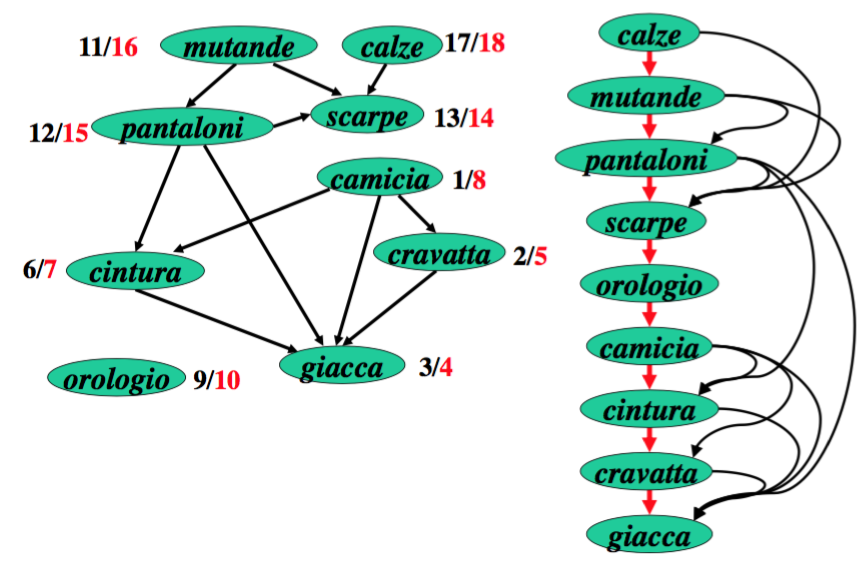
\includegraphics[width=.5\textwidth]{./notes/immagini/l7-fig1.png}
\end{figure}

\section{Un primo modello lineare}\label{un-primo-modello-lineare}

Ipotizzando che ci sia una relazione lineare è possibile utilizzare il
modello del capitolo precedente:

$$
y = \alpha + \beta x + \epsilon
$$

$$
\hat{\beta} = \frac{\cov(X,Y)}{\var(X)} \qquad \hat{\alpha} = \bar{y} - \hat{\beta}\bar{x}
$$

Utilizzando l'ambiente R si ottengono delle informazioni relative all
modello ottenuto:

\begin{verbatim}
lm(formula = gas ~ prezzo)
Residuals:
    Min      1Q  Median      3Q     Max
-40.625 -10.719  -1.136  14.073  38.292
Coefficients:
            Estimate Std. Error t value Pr(>|t|)
(Intercept)  138.561     13.552  10.225 6.34e-09 ***
prezzo        -1.104      0.202  -5.467 3.42e-05 ***
---
Signif. codes:  0 ‘***’ 0.001 ‘**’ 0.01 ‘*’ 0.05 ‘.’ 0.1 ‘ ’ 1
Residual standard error: 20.86 on 18 degrees of freedom
Multiple R-Squared: 0.6241,     Adjusted R-squared: 0.6033
F-statistic: 29.89 on 1 and 18 DF,  p-value: 3.417e-05
\end{verbatim}

Dai dati si può notare che l'indice $ R^2 $ è uguale a 0.62, il che indica un buon andamento lineare.
Inoltre come \textit{p-value} si ottiene un valore molto basso, il che porta a rifiutare l'ipotesi nulla.

Tracciando però i grafici dei residui è possibile osservare c'è una componente indipendente che non è lineare.

\begin{figure}[htbp]
	\centering
	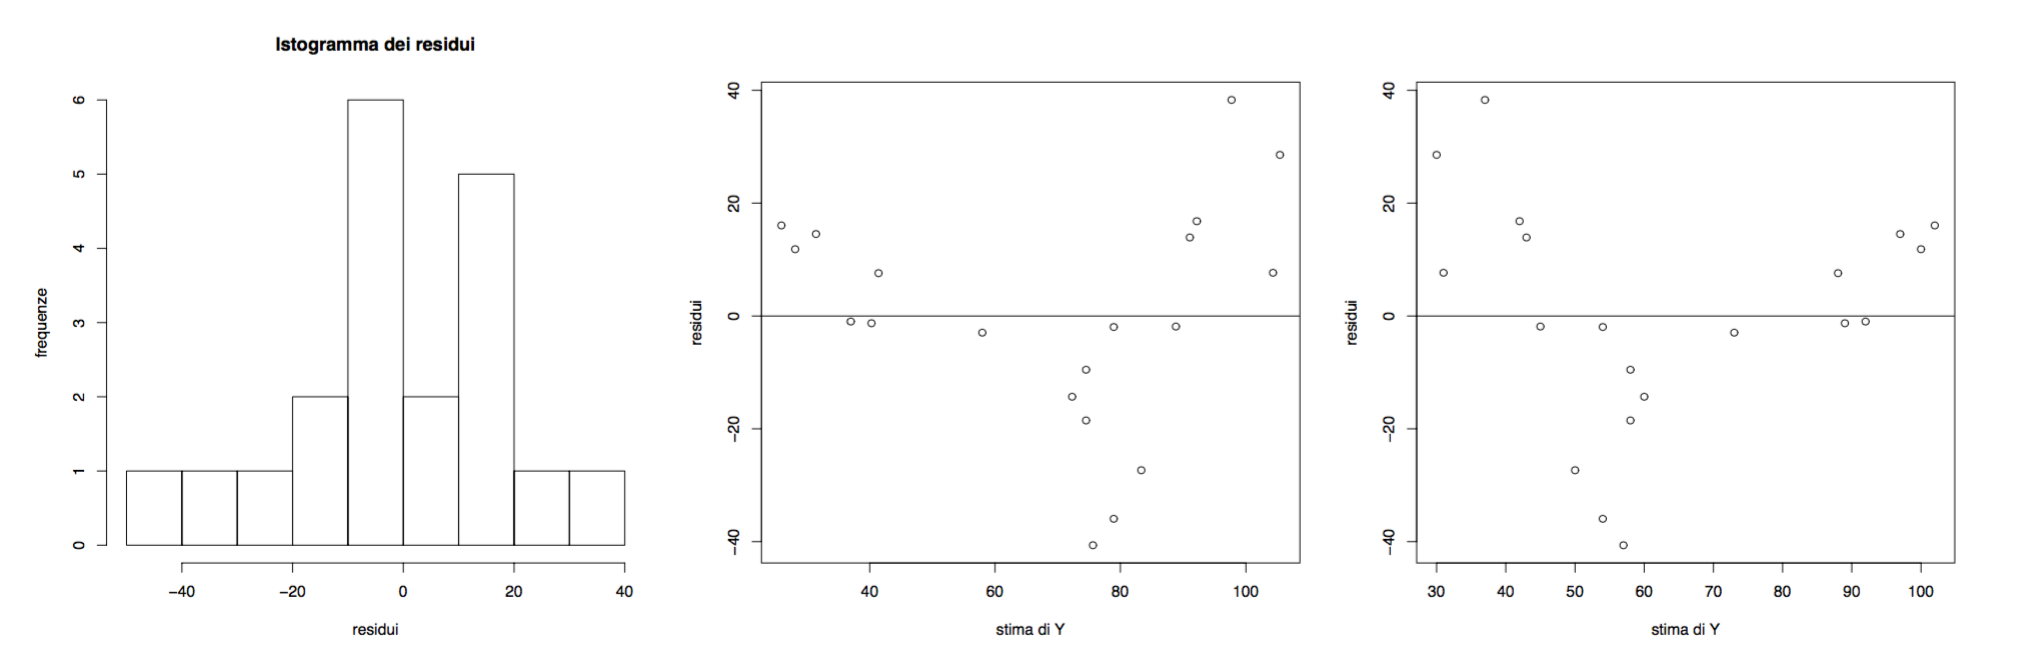
\includegraphics[width=1\textwidth]{./notes/immagini/l7-fig2.png}
	\caption{Tracciamento dei residui per il primo modello. \`{E} possibile notare la presenza di indipendente.}
\end{figure}

\section{Considerazioni sul problema e un secondo modello}\label{considerazioni-sul-problema-e-un-secondo-modello}

Considerando il problema modellato è possibile fare alcune osservazioni:

\begin{itemize}
	\item il consumatore potrebbe destinare solamente un determinato budget $ \kappa $ per l'acquisto del gas, ovvero $ x \cdot y = \kappa $.
	\item è ragionevole pensare che il consumatore debba consumare una quantità minima di gas $ \gamma $
	\item essendo il mercato del gas regolamentato, c'è un prezzo minimo di $ 7 $ centesimi al metro cubo sotto il quale non è possibile vendere il gas.
\end{itemize}

Tenendo in considerazione quanto elencato si arriva ad avere l'equazione:

$$
(x-7)(y-\gamma) = \kappa
$$

la quale può essere riscritta in un modo più simile a quella del modello lineare

$$
y = \gamma + \kappa \cdot \frac{1}{x-7}
$$

e sostituendo la variabile \textit{x} con $ z = \frac{1}{x-7} $, si ottiene proprio la stessa equazione la quale permette di calcolare la retta ai minimi quadrati.

Questo è possibile perché quello che finora è stato chiamato modello lineare è un caso particolare dei \textbf{modelli lineari nei parametri}. Ovvero la limitazione data dalla linearità non riguarda le variabili, ma riguarda solamente i \textbf{parametri} del modello.

Quando viene utilizzato il metodo dei minimi quadrati con questi modelli è necessario tenere in considerazione le trasformazioni che vengono fatte alle variabili, perché i valori calcolati ai minimi quadrati riguardano le variabili trasformate e non quelle di partenza, è necessario quindi \textbf{scalare} in modo opportuno i valori\footnote{Se viene scalata solamente la $ x $ non c'è questo problema perché i minimi quadrati considerano solamente le distanze rispetto l'asse $ y $.}.

La formulazione più generale del modello lineare è quindi

$$
g(y) = \alpha + \beta h(x) + \epsilon
$$

Il modello ottenuto per la nuova formulazione è:
\begin{verbatim}
lm(formula = gas ~ I(1/(prezzo - 7)))
Residuals:
Min    1Q  Median  3Q    Max
-29.617 -4.574 2.394 7.800 30.917
Coefficients:
Estimate Std. Error t value Pr(>|t|) 
(Intercept) 3.918 8.376 0.468 0.646
I(1/(prezzo - 7)) 3034.938 357.037 8.500 1.02e-07 *** 
---
Signif. codes: 0 ‘***’ 0.001 ‘**’ 0.01 ‘*’ 0.05 ‘.’ 0.1 ‘ ’ 1
Residual standard error: 15.19 on 18 degrees of freedom 
Multiple R-Squared: 0.8006, Adjusted R-squared: 0.7895 
F-statistic: 72.26 on 1 and 18 DF, p-value: 1.022e-07
\end{verbatim}

ovvero la retta

$$
y = 3.918 + 3034.938 \cdot \frac{1}{x-7}
$$

\begin{figure}[htbp]
	\centering
	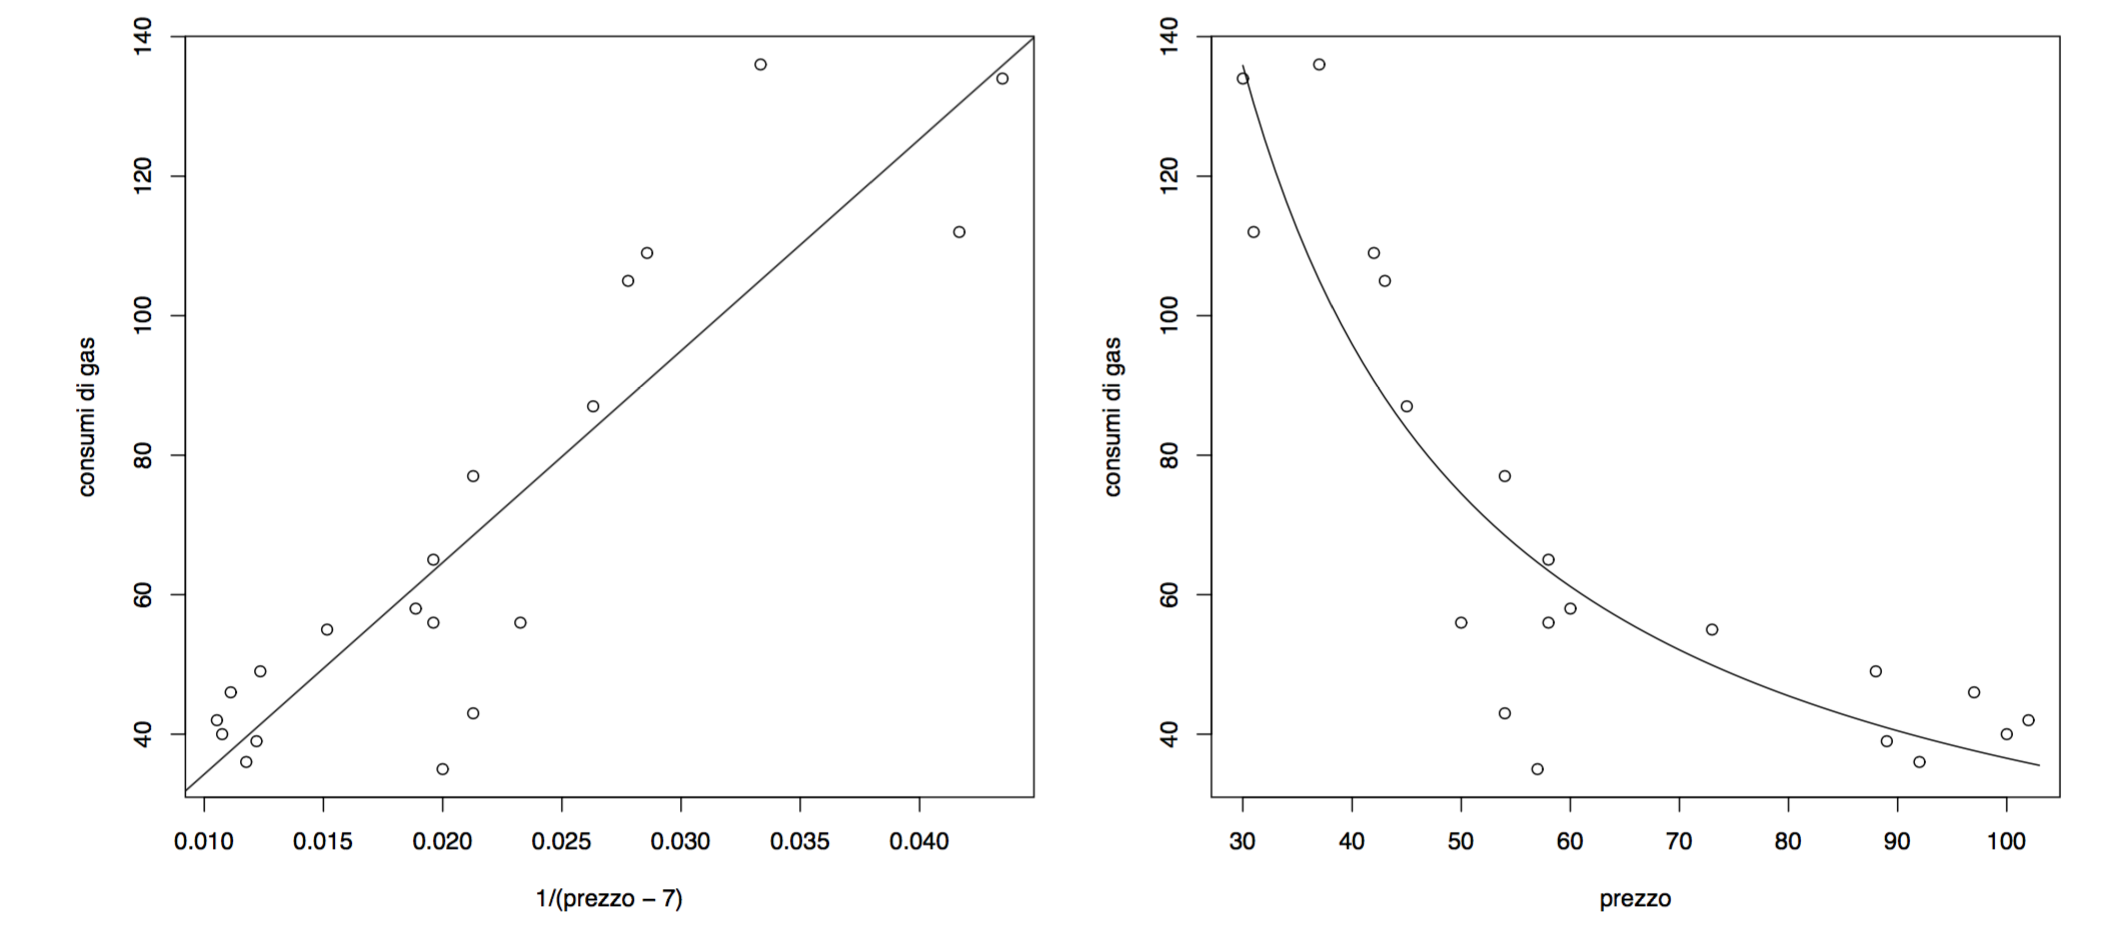
\includegraphics[width=1.1\textwidth]{./notes/immagini/l7-fig3.png}
	\caption{A destra la retta rispetto $ z $. A sinistra il modello lineare tracciato rispetto $ x $.}
\end{figure}

Dai dati del nuovo modello è possibile osservare che la varianza residua (\texttt{Residual standard error} elevato al quadrato) è passata da circa 391 a circa 207, ovvero il quadrato degli errori di previsione è stato ridotto di quasi il $ 50\% $.
Lo stesso effetto può essere visto utilizzando $ R^2 $ che da 0.6241 passa a 0.8006.

\begin{figure}[htbp]
	\centering
	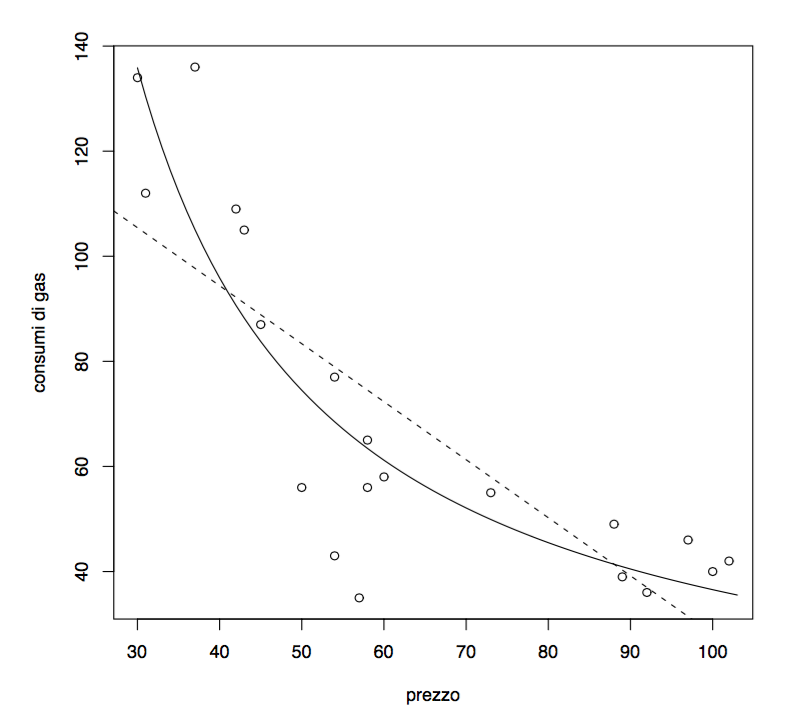
\includegraphics[width=.6\textwidth]{./notes/immagini/l7-fig4.png}
	\caption{Confronto grafico tra i due modelli.}
\end{figure}

\FloatBarrier
\section{Modello lineare con trasformate}\label{modello-lineare-con-trasformate}

\textit{Cambia il dataset di riferimento}, si vuole controllare se il reddito nazionale influisce sulla speranza di vita media dello stato. 

\begin{figure}[htbp]
	\centering
	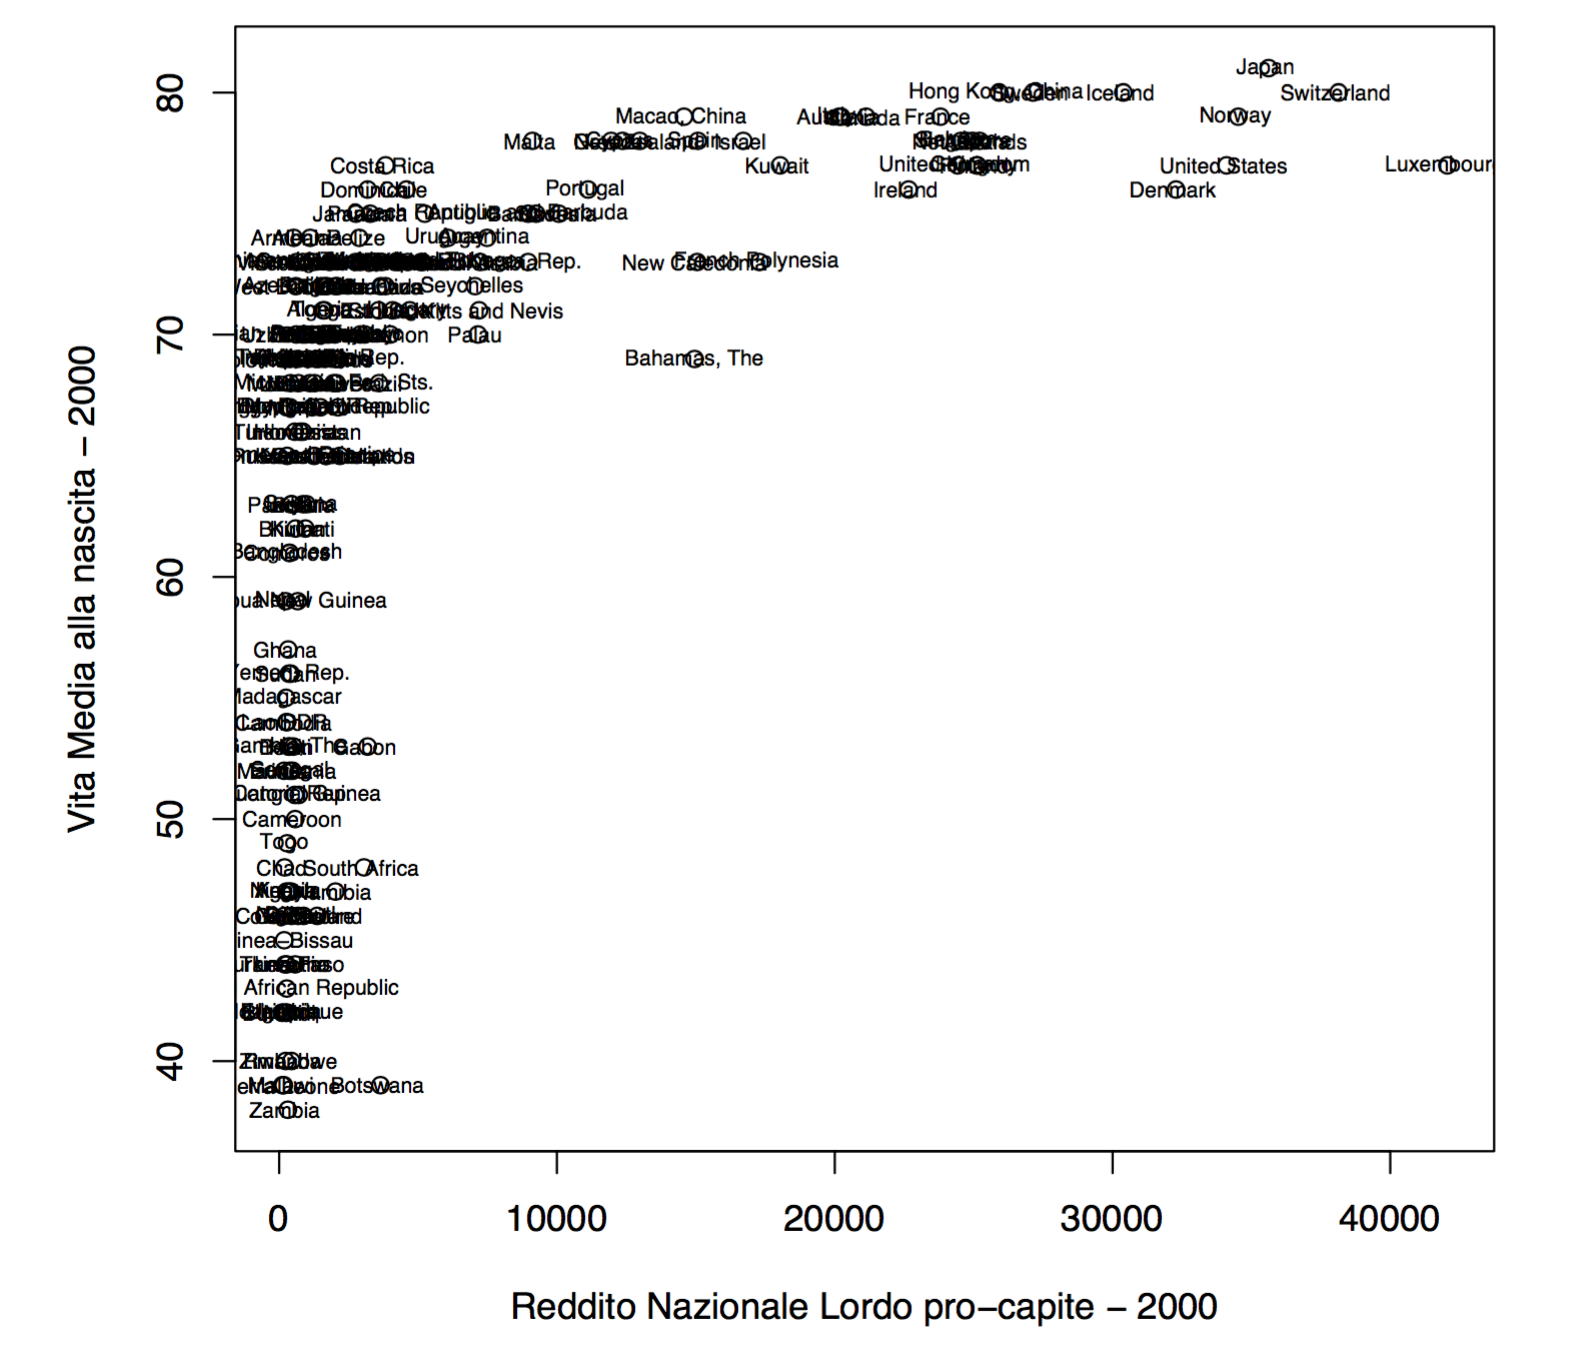
\includegraphics[width=.7\textwidth]{./notes/immagini/l7-fig5.png}
	\caption{Dataset - GNI - ELF}
\end{figure}

La prima cosa da fare è osservare come si comporta il modello lineare senza trasformazioni:

\begin{verbatim}
	lm(formula = elf ~ GNIpc)
	Residuals:
	Min    1Q  Median  3Q    Max
	-24.924 -7.512 4.119 7.431 12.948
	Coefficients:
	Estimate Std. Error t value Pr(>|t|)
	(Intercept) 6.133e+01 8.967e-01 68.390 < 2e-16 ***
	GNIpc 7.115e-04 8.230e-05 8.645 3.76e-15 ***
	---
	Signif. codes: 0 ‘***’ 0.001 ‘**’ 0.01 ‘*’ 0.05 ‘.’ 0.1 ‘ ’ 1
	Residual standard error: 9.903 on 171 degrees of freedom 
	Multiple R-Squared: 0.3041, Adjusted R-squared: 0.3 
	F-statistic: 74.73 on 1 and 171 DF, p-value: 3.757e-15
\end{verbatim}

Si può notare come l'indice $ R^2 $ sia molto basso (0.3041), ma risulta essere molto significativo perché, per il \textit{p-value} ottenuto sia ha che è improbabile che valga l'ipotesi nulla.

Tracciando il modello e il grafico dei residui è possibile notare che
\begin{itemize}
	\item La retta ottenuta non curva abbastanza e quindi non si adatta bene ai dati
	\item Il modello prevede una vita media che può essere maggiore di 90 anni, il che è abbastanza improbabile.
\end{itemize}

\begin{figure}[htbp]
	\centering
	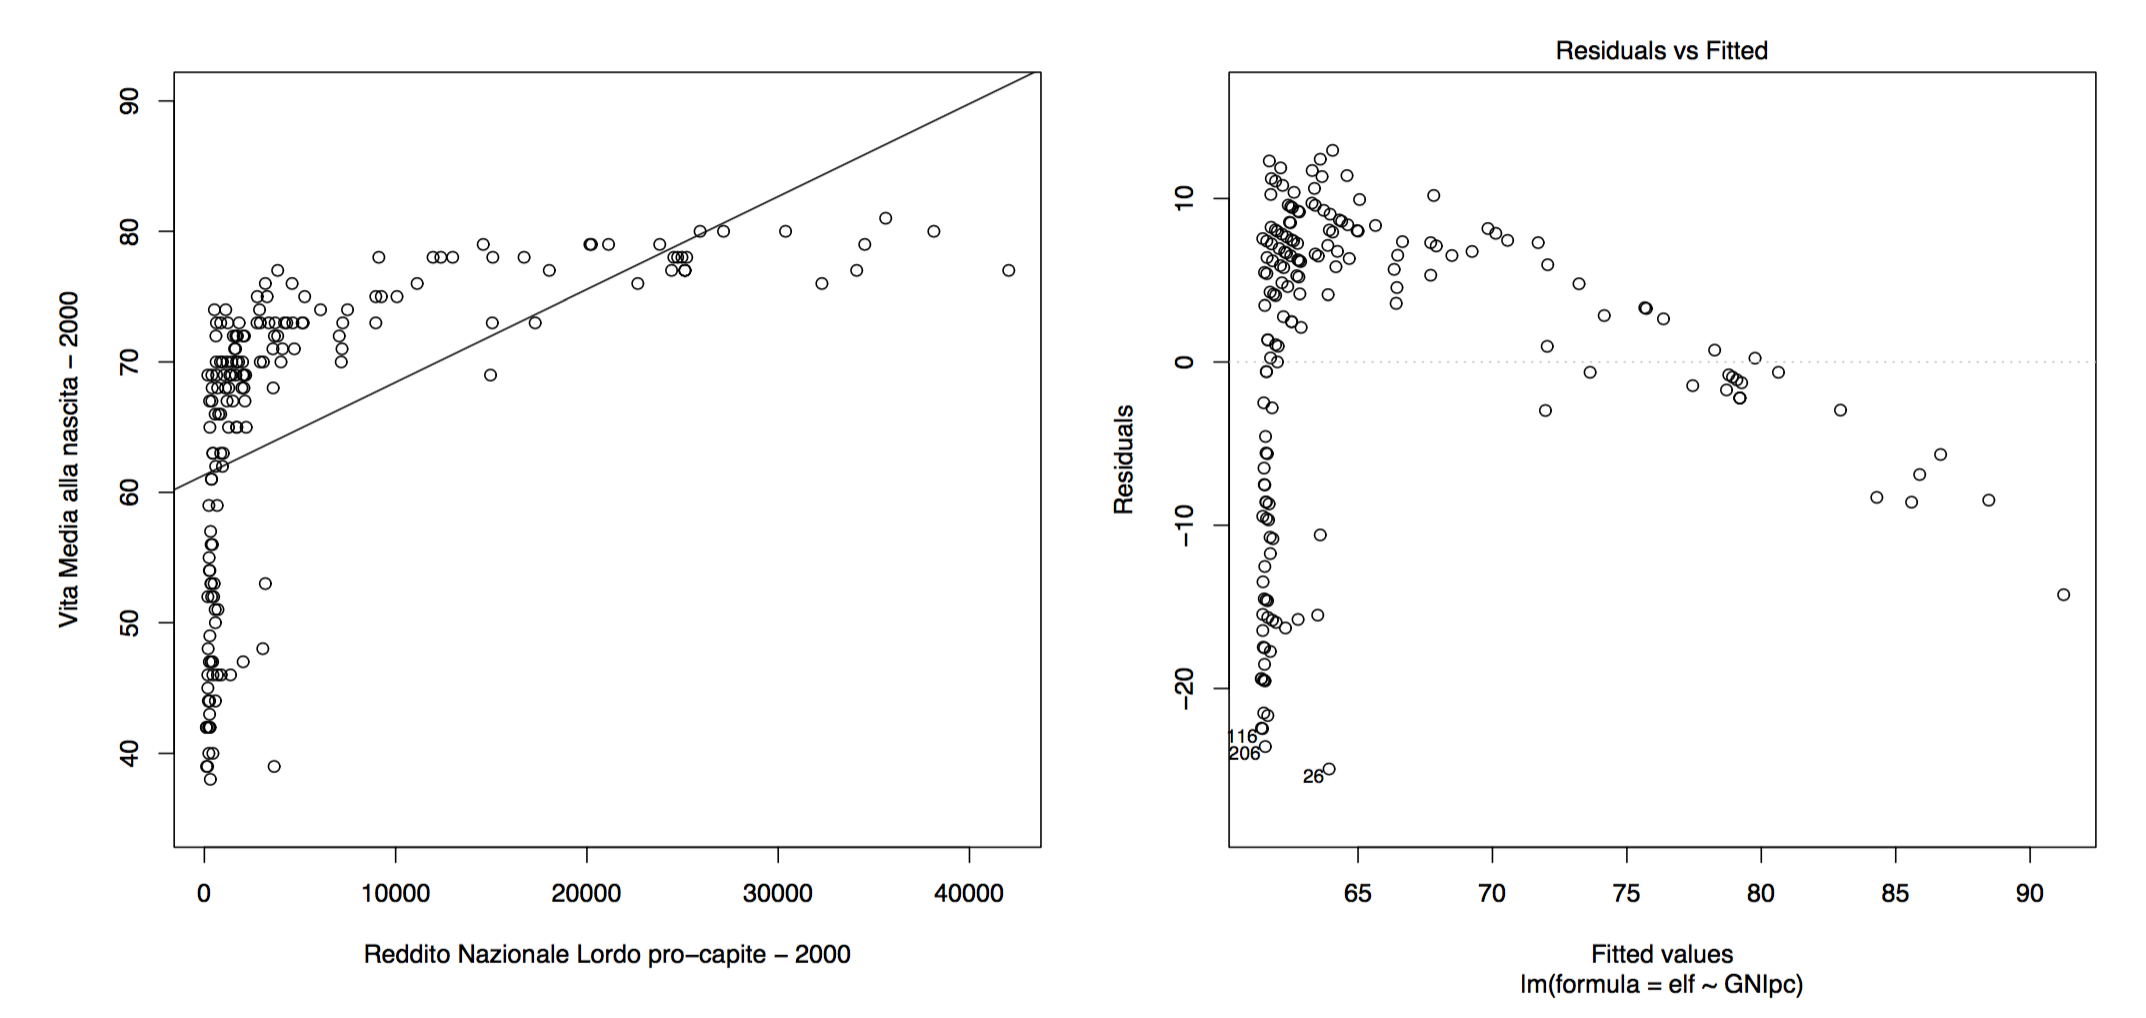
\includegraphics[width=.9\textwidth]{./notes/immagini/l7-fig6.png}
	\caption{Primo modello e residui ottenuti}
\end{figure}

Per adattare meglio la curva è possibile utilizzare la scala logaritmica per l'asse delle \textit{x}. In questo modo, al crescere del reddito viene dato via via meno peso.
Inoltre, rappresentando graficamente questa trasformazioni si ottiene una nuvola di punti più simile ad una retta.

\begin{figure}[htbp]
	\centering
	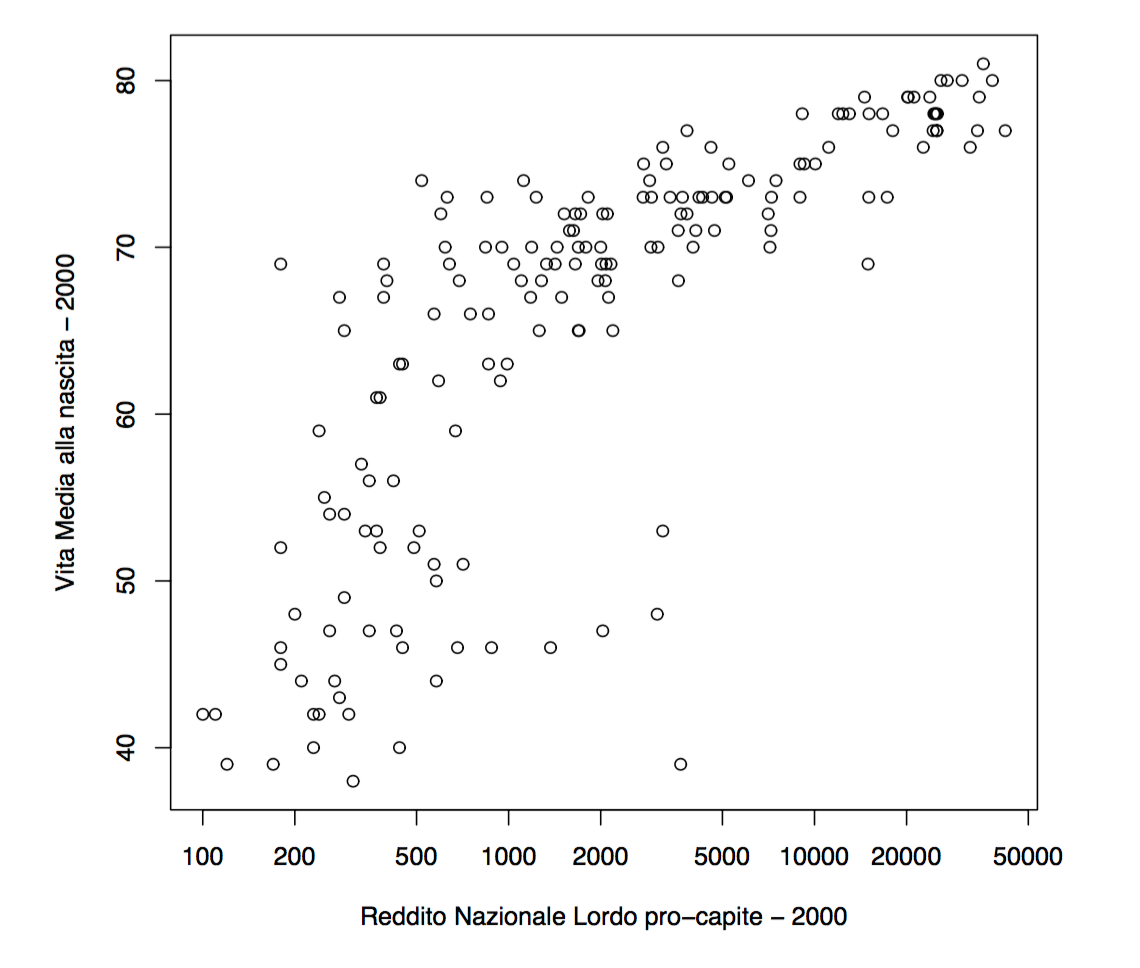
\includegraphics[width=.6\textwidth]{./notes/immagini/l7-fig7.png}
	\caption{Grafico che utilizza la scala logaritmica per i valori delle $ x $. L'asse è comunque etichettato con i valori originali.}
\end{figure}

Il modello diventa quindi

$$
(\text{vita media alla nascita}) = \alpha + \beta \log(\text{reddito nazionale pro capite})
$$

\begin{verbatim}
lm(formula = elf ~ I(logGDP), data = elf.data)
Residuals:
Min     1Q   Median   3Q     Max
-29.6591 -2.9511 0.7906 5.1050 17.4844
Coefficients:
Estimate Std. Error t value Pr(>|t|)
(Intercept) 22.6701 2.8447 7.969 2.02e-13 *** 
I(logGDP) 5.6767 0.3677 15.438 < 2e-16 ***
---
Signif. codes: 0 ‘***’ 0.001 ‘**’ 0.01 ‘*’ 0.05 ‘.’ 0.1 ‘ ’ 1
Residual standard error: 7.674 on 174 degrees of freedom 
Multiple R-Squared: 0.578, Adjusted R-squared: 0.5756 
F-statistic: 238.3 on 1 and 174 DF, p-value: < 2.2e-16
\end{verbatim}

Con questo secondo modello si ottiene un indice $ R^2 $ doppio rispetto al precedente e questo può essere osservato anche nella rappresentazione grafica del nuovo modello.

\begin{figure}[htbp]
	\centering
	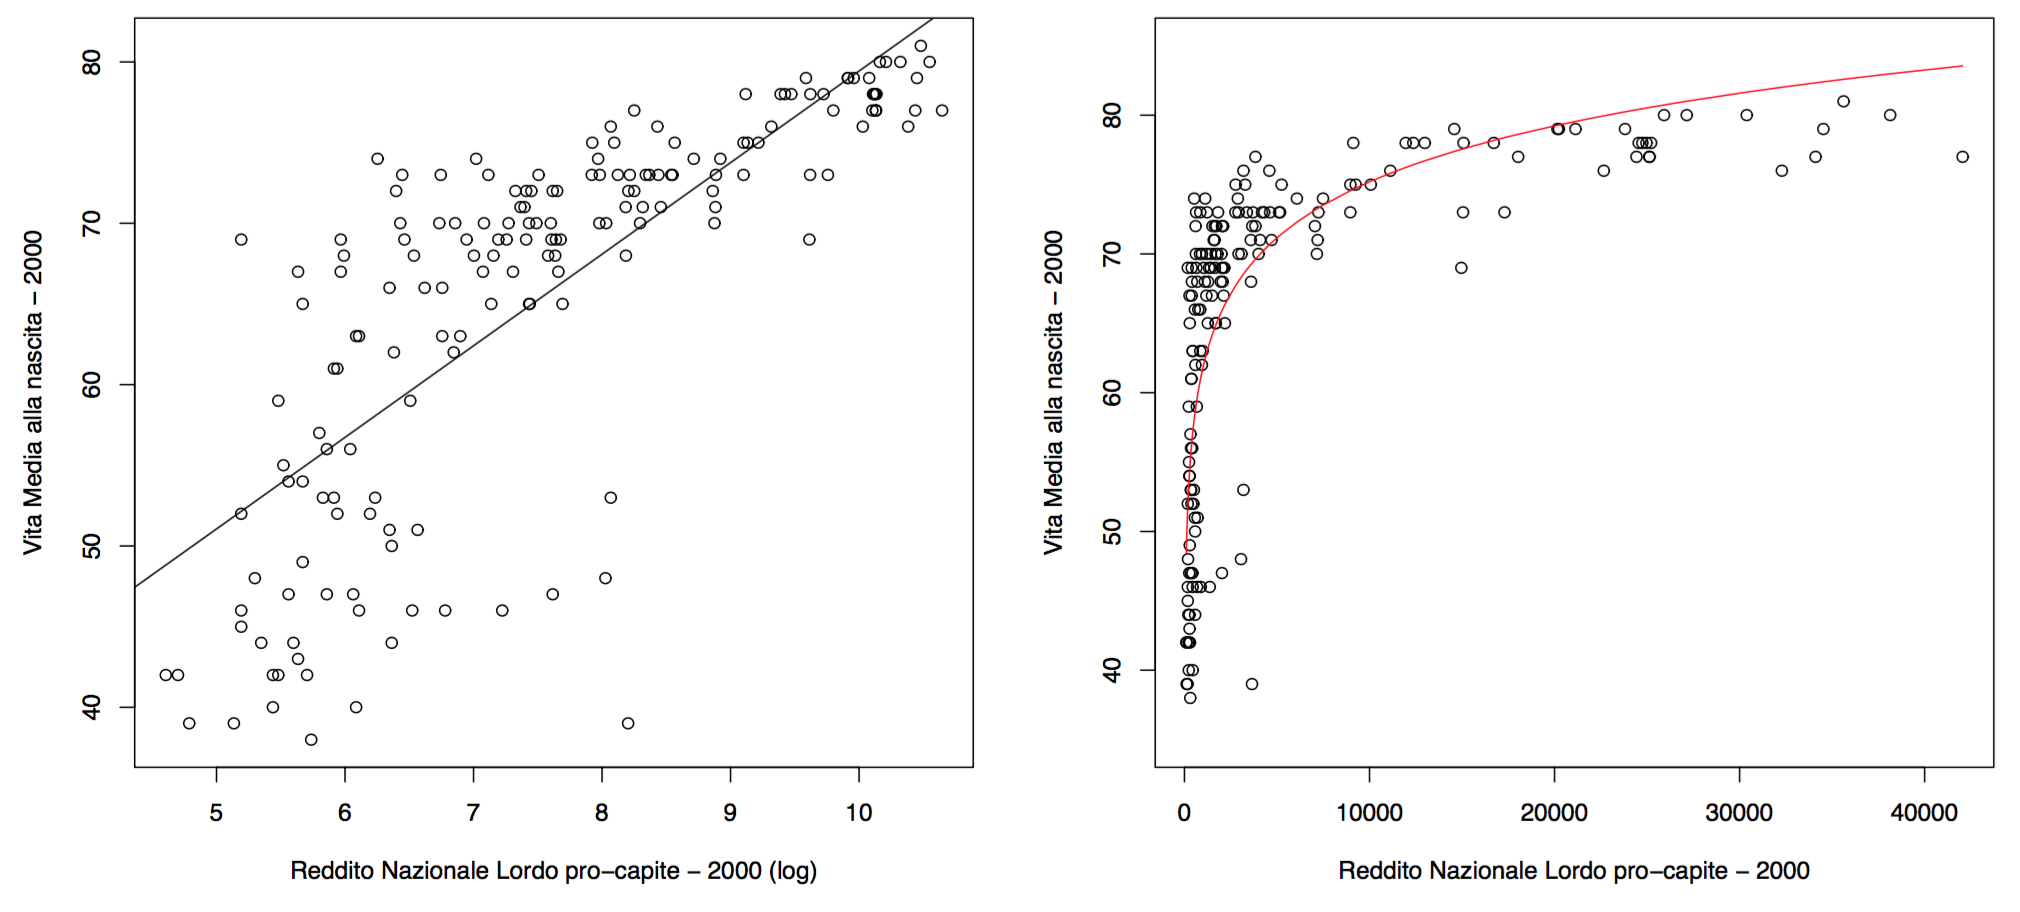
\includegraphics[width=.9\textwidth]{./notes/immagini/l7-fig8.png}
	\caption{Secondo modello: a sinistra con la scala logaritmica, a destra normale.}
\end{figure}

C'è però ancora un problema che riguarda i valori estremi che non vengono approssimati bene dalla curva e lo si può notare anche dai residui.

\begin{figure}[htbp]
	\centering
	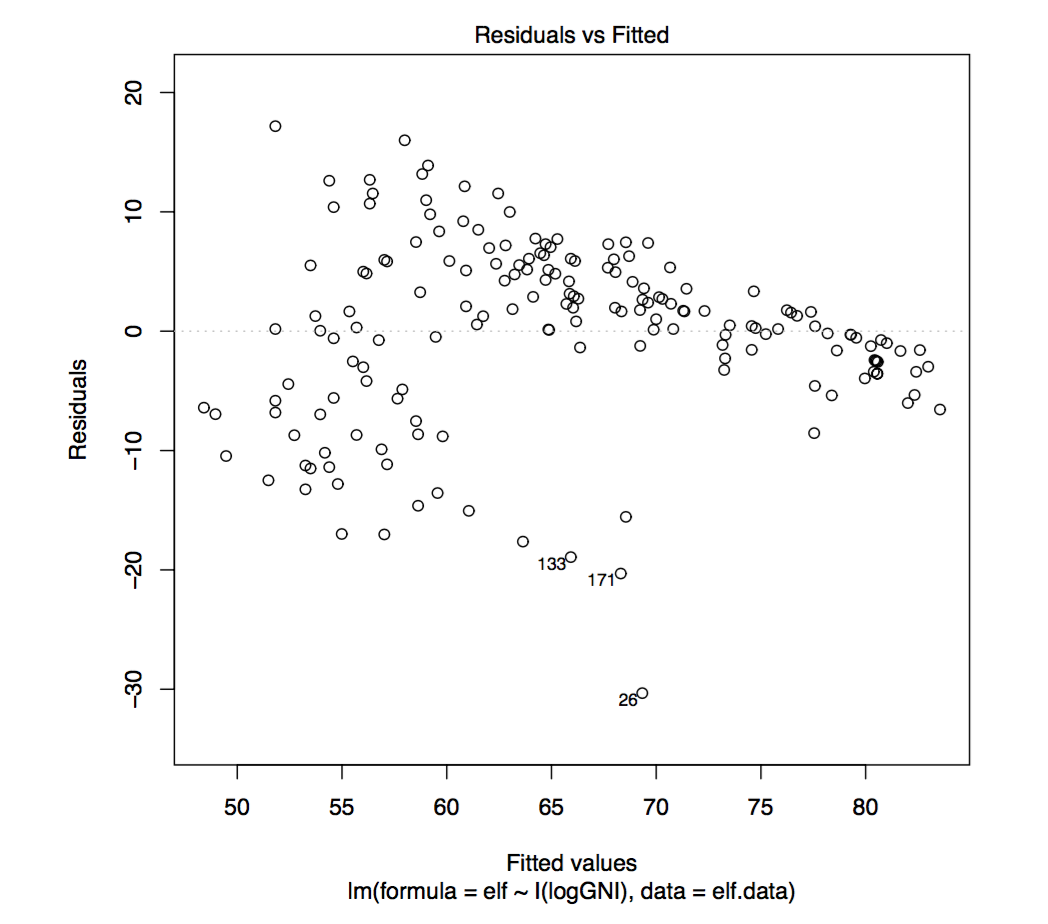
\includegraphics[width=.6\textwidth]{./notes/immagini/l7-fig9.png}
	\caption{Residui per il secondo modello }
\end{figure}

Un'ulteriore modifica può essere quella di trasformare anche la variabile risposta, elevandola alla quinta, in modo da dare maggior peso ai valori maggiori.

Il modello ottenuto è quindi dato da

$$
(\text{vita media alla nascita})^5 = \alpha + \beta \log(\text{reddito nazionale pro capite}) + \epsilon
$$

Da notare che con questa formulazione le ipotesi sugli errori (media nulla, varianza costante, distribuzione normale, ecc.) \textbf{devono valere per gli errori su scala trasformata}.

Una volta calcolato il modello si ottiene

\begin{verbatim}
lm(formula = elf.5 ~ logGNI, data = elf.data)
Residuals:
Min        1Q        Median    3Q       Max
-1.801e+09 -2.817e+08 7.965e+06 3.036e+08 1.334e+09
Coefficients:
Estimate Std. Error t value Pr(>|t|) 
(Intercept) -2.345e+09 1.832e+08 -12.80 <2e-16 *** 
logGNI 5.164e+08 2.376e+07 21.73 <2e-16 ***
---
Signif. codes: 0 ‘***’ 0.001 ‘**’ 0.01 ‘*’ 0.05 ‘.’ 0.1 ‘ ’ 1
Residual standard error: 4.89e+08 on 171 degrees of freedom 
Multiple R-Squared: 0.7341, Adjusted R-squared: 0.7326 
F-statistic: 472.2 on 1 and 171 DF, p-value: < 2.2e-16
\end{verbatim}

\begin{figure}[htbp]
	\centering
	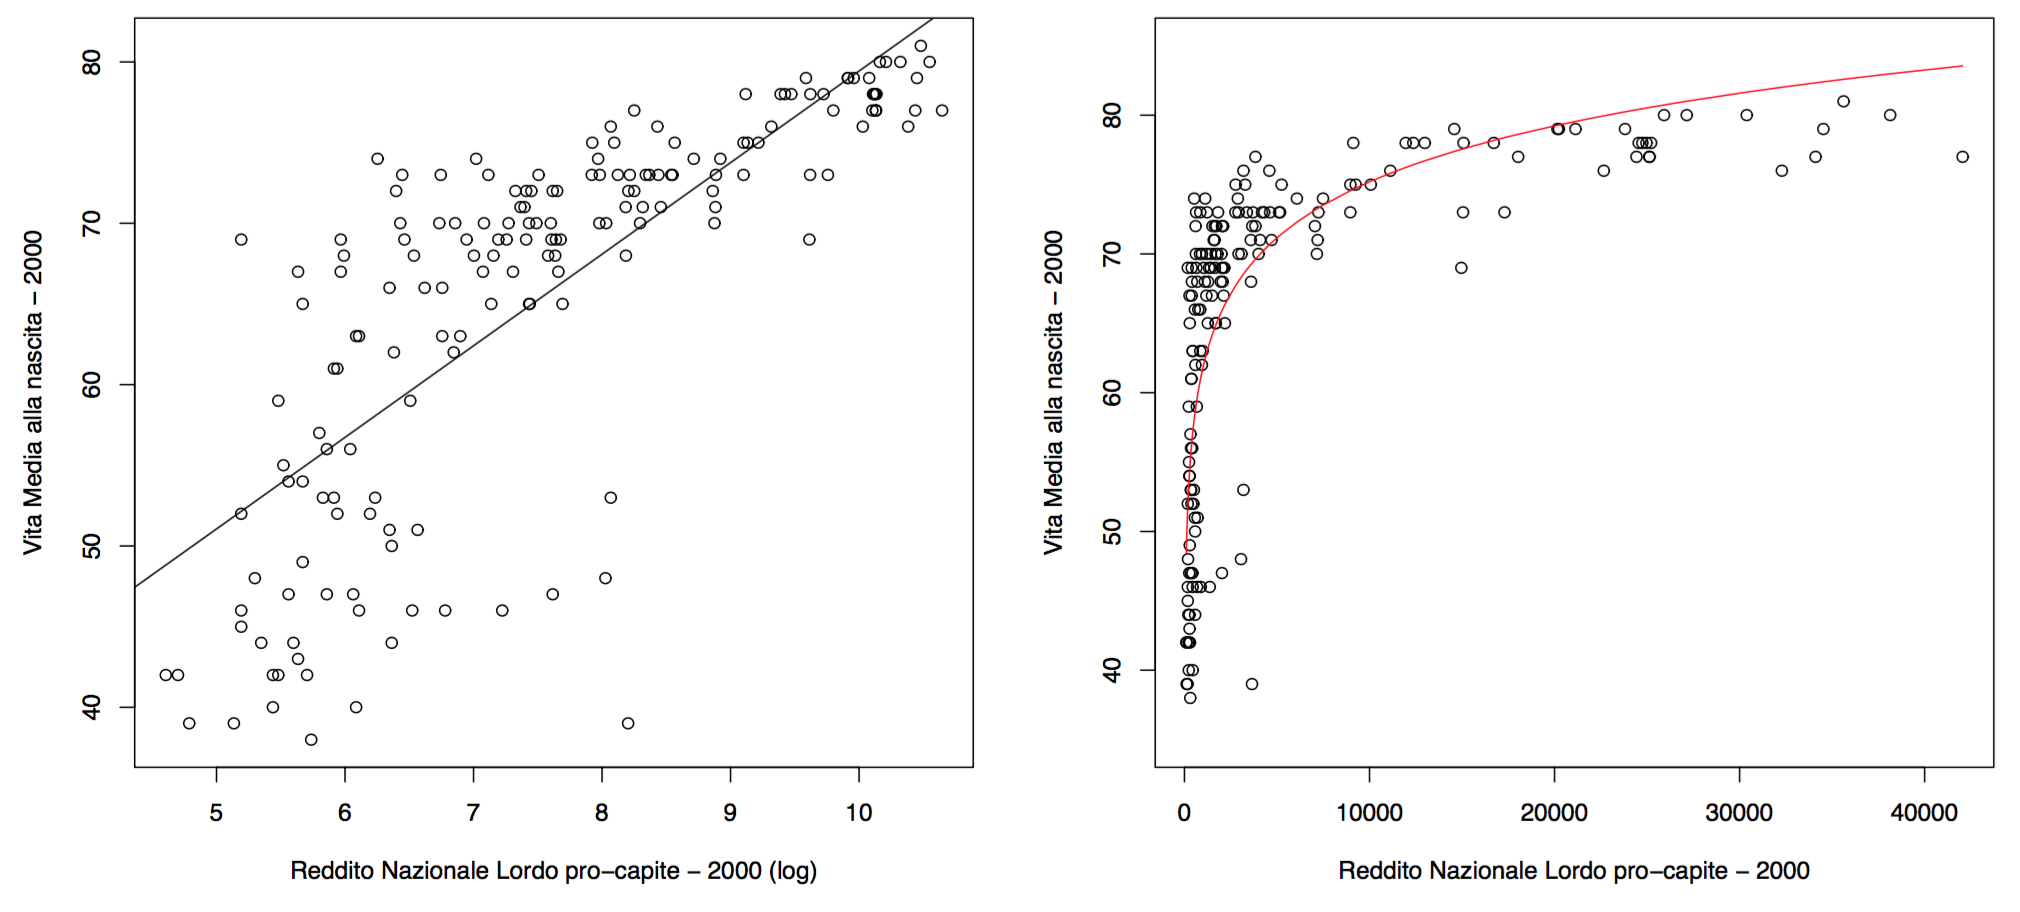
\includegraphics[width=.9\textwidth]{./notes/immagini/l7-fig8.png}
	\caption{Terzo modello: a sinistra con la scala originale e a destra i residui.}
\end{figure}

L'indice $ R^2 $ ottenuto fa riferimento ai residui calcolati sulla scala trasformata, quindi per avere un'indice di adattamento dei dati è possibile utilizzare la media dei quadrati dei residui per la variabile originale:

$$
\frac{1}{n}\sum\limits_{i=1}^n \bigg[ \big(\text{vita media alla nascita}\big)_i - \sqrt[5]{\big(\alpha + \beta \log(\text{reddito nazionale pro capite})_i\big)}\bigg]^2
$$

Calcolando questo valore si ottiene 55.08, mentre con il secondo modello si aveva la varianza dei residui pari a 58.89. Si ottiene quindi una riduzione del $ 6\% $ del quadrato degli errori di previsione.










	% !TEX encoding = UTF-8
% !TEX program = pdflatex
% !TEX root = AALP.tex
% !TEX spellcheck = it-IT

% 27 Ottobre 2016
%\section{Estensioni del nostro linguaggio}
%\subsection{Record}
% \subsubsection{L'oggetto conto}

\section{Tipi variante}

Se i record possono essere visti come tipi congiunzione, che combinano più tipi, i tipi variante possono essere visti come disgiunzione.

Ad esempio possiamo pensare ad un contatto in una rubrica che può avere un indirizzo fisico o virtuale:

$$
< \text{fisico}: \underbrace{\{ \text{nome : String}, \text{indirizzo: String} \}}_{T_{fisico}} , \: \text{virtuale}: \underbrace{\{ \text{login : String}, \text{email : String} \}}_{T_{virt}} >= T_{ind}
$$

\noindent Un esempio di valore che ha questo tipo è:

$$
< \text{fisico} = \{ \text{nome = ``pippo''}, \text{indirizzo =  ``Via rosa''} \} >
$$

\noindent L'utilità di questi tipi si ha con l'operatore di pattern matching.
Ad esempio in Scala è possibile definire delle funzione generiche che lavorano sui tipi variante:

\begin{lstlisting}[language=Scala, caption=Utilizzo del pattern matching in Scala]
def getName(a : Tind) : String = a match{
	case <fisico = x> => x.nome
	case <virtuale = x> => x.login
	/** case <l = x> => ... da errore di compilazione! */
	/** allo stesso modo viene segnalato se il pattern non copre tutte le possibili etichette */
}

def getAll(a : List[Tind] ) : List[String] = {
	var l = new List[String]
	for (x <- a) l.add(getName(x))
}
\end{lstlisting}

\noindent Per inserire nel nostro linguaggio questi valori servono dei nuovi termini:

$$
M ::= < l = M > \vbar M \text{ match } \{\text{case }l_i = x_i => M_i \:^{i = 1\ldots n}\} \vbar \ldots
$$

\noindent Da notare che la $x_i$ che viene utilizzata nel \text{match} lega le eventuali occorrenze all'interno di $M_i$.

$$
<l_1 = 3> \text{ match } \{\text{case } l_1 = x => x+1, \ldots \} \rightarrow 3+1
$$

\noindent Più formalmente:

\begin{itemize}
	\item $fv(<l =M>) = fv(M)$
	\item $fv( M \text{ match } \{\text{case }l_i = x_i => M_i \:^{i = 1\ldots n}\}) = fv(M) \cup \bigcup_{i = 1 \ldots n}\bigg( fv(M_i) \setminus \{x_i\} \bigg) $
\end{itemize}


\noindent Servono inoltre dei nuovi valori finali e dei tipi:

$$
v ::= <l = v> \vbar \ldots \qquad T ::= < l_i : T_i \:^{i = 1 \ldots n}>
$$

\noindent La semantica operazionale viene espressa con 3 nuove regole:

\begin{itemize}
	\item Riduzione del termine interno
	\begin{prooftree}
		\AxiomC{$M \rightarrow M'$}
		\LL{Variant}
		\UnaryInfC{$<l = M> \rightarrow <l = M'>$}
	\end{prooftree}
	\item Avanzamento in un match:
	\begin{prooftree}
		\AxiomC{$M \rightarrow M'$}
		\LL{Red-Match}
		\UnaryInfC{$M \text{ match } \{\text{case } l_i = x_i => M_i \:^{i = 1 \ldots n}\} \to M' \text{ match } \{\text{case } l_i = x_i => M_i \:^{i = 1 \ldots n}\}$}
	\end{prooftree}
	\item Assioma per il match effettivo
	\begin{prooftree}
		\AxiomC{$j \in \{1 \ldots n\}$}
		\LL{Match}
		\UnaryInfC{$<l_j = v> \text{ match } \{\text{case } l_i = x_i => M_i \:^{i = 1 \ldots n}\} \rightarrow M_j\{x_j = v\}$}
	\end{prooftree}
\end{itemize}

\noindent Servono inoltre delle regole di tipo, una per l'invariante e l'altra per il match.

\begin{prooftree}
	\AxiomC{$ \Gamma \vdash M: T_j $}
	\AxiomC{$ j \in \{1 \ldots n \} $}
	\LL{Type-Variant}
	\BinaryInfC{$\Gamma \vdash <l_j = M> : <l_i : T_i \:^{i=1\ldots n}>$}
\end{prooftree}

\noindent Con questa regola posso assegnare ad un valore infiniti tipi, l'importante è che in questi infiniti tipi ci sia l'etichetta $l_j$ in modo da avere la garanzia di riuscire ad effettuare il pattern matching.

\begin{prooftree}
	\AxiomC{$\Gamma \vdash M : < l_i : T_i  \:^{i=1\ldots n}>$}
	\AxiomC{$\Gamma, x_i : T_i \vdash M_i : T \:\: \forall \: i = 1 \ldots n $}
	\LL{Type-Match}
	\BinaryInfC{$\Gamma \vdash M \text{ match }\{\text{case }l_i = x_i => M_i \:^{i=1\ldots n}\} : T$}
\end{prooftree}

\noindent Perché un match sia ben tipato è necessario che il termine $M$ sia un valore di tipo variante e che tutti i ``rami'' del match siano termini con lo stesso tipo, aggiungendo anche al contesto la sostituzione che viene effettuata quando viene applicato il match.

Se nel pattern matching ho come premessa della regola $\Gamma \vdash M : < l_i : T_i  \:^{i=1\ldots m}>$ con $m \geq n$ c'è un problema perché possono capitare delle etichette che il costrutto \text{match} non riesce a gestire. Se invece $m \leq n$ non ci sono problemi. Ma anche in questo caso, dato che ho a disposizione infiniti tipi, conviene forzare $m = n$.

Anche se non sembra questi tipi sono presenti nella maggior parte dei linguaggi main stream, solo che questi vengono nascosti da dello zucchero sintattico. Ad esempio le liste possono essere viste come un tipo variante in quanto sono o una lista vuota o la concatenazione di un elemento e un'altra lista.

$$
\text{List} = < \text{nil : Unit}, \text{cons} : (\Nat * \text{List}) >
$$

\noindent Si tratta di un tipo ricorsivo che non è supportato nella nostra grammatica, ma in altre grammatiche è possibile gestirlo.

I valori per questo tipo sono:

$$
<\text{nil } = \text{unit}>  \quad <\text{cons} = (5, <\text{nil } = \text{unit}>)>
$$

\noindent Un altro caso d'uso dei valori variante è l'analisi delle dereferenziazioni dei valori null.
Ad esempio in Java possiamo definire una variabile e assegnarle null:

\begin{lstlisting}[language=Java]
C c = null;

C find(List<C> l, C a) { ... } // se non trova ritorna null

C c = find(list, s);
// c può essere null, quindi devo controllare
// se non controllo potrei finire in un NullPointerException, anche perché il compilatore non controlla questo tipo di eccezioni
if (c != null) print(c.info());
else print("non trovato");
\end{lstlisting}

\noindent Questo approccio non è dei migliori, perché dovrebbe utilizzare le eccezioni personalizzate, ma si è visto che nessuno le usa. Con C\# si sono invece inventati i tipi \texttt{Nullable} che possono avere anche come valore \texttt{Null}, anche per i tipi primitivi.

Un'altra idea è stata quella di introdurre i tipi \texttt{!}: una classe di tipo \texttt{C!} non può assumere come valore null, in modo da sfruttare di più l'analisi statica.

Linguaggio che vai, soluzione che trovi. Altri linguaggi utilizzano i così detti \textbf{null objects}:

\begin{lstlisting}[language=Java]
class C {
	...
	String info() {...}
	...
}
class NullC extends C {
	...
	String info() {}
}
\end{lstlisting}

\noindent Così facendo c'è un metodo definito da chiamare anche sul valore null, in modo da evitare la NullPointerExcpetion.

Scala e Java8 (e Swift) implementano un'ulteriore versione, gli \textbf{option type}, ovvero un tipo variante che prevede due possibilità: c'è l'oggetto oppure non c'è.
La definizione di questo tipo è la seguente:

$$
Option[C] = < \text{none} : \text{Unit}, \text{some} : C >
$$

\noindent Il codice di prima può essere quindi riscritto come

\begin{lstlisting}[language=Scala]
...
def find(l : List[C], s : String) : Option[C] = {
	for(x <- l) 
		if (x.info() == s) return Some(x)
	return None 
}
...
find(l, "pippo") match {
	case Some(x) => print(x.info())
	case None => print("non trovato")
}
\end{lstlisting}

\noindent Si può notare come questa versione del codice è più espressiva e si riesce subito a capire che la funzione \texttt{find} può non trovare l'elemento cercato.



	% !TEX encoding = UTF-8
% !TEX TS-program = pdflatex
% !TEX root = computabilità e algoritmi.tex
% !TEX spellcheck = it-IT
\section{Composizione generalizzata}\label{composizione-generalizzata}

$$f: \mathbb{N}^k \rightarrow \mathbb{N},\: g_1,\ldots g_n : \mathbb{N}^k \rightarrow \mathbb{N}$$

La loro composizione $h: \mathbb{N}^k \rightarrow \mathbb{N}$ è data da: 

$$
h(\vec{x}) = f(g_1(\vec{x}), \ldots, g_n(\vec{x}))
$$

La funzione $h(\vec{x})\downarrow$ (è definita) se tutte le
$g_i \downarrow y_i, f(y_1,\ldots,y_n) \downarrow$.

L'approccio utilizzato nella valutazione delle funzioni è quello
\textbf{eager}, ovvero vengono valutati prima tutti i parametri.

Ad esempio: $\underline{0} : \mathbb{N} \rightarrow \mathbb{N},\: \underline{0}(x) = 0$ e $d(x) = \uparrow,\: \underline{0}(d(1))$ è
$\uparrow$ perché prima è necessario valutare i parametri.

\subsection{Calcolabilità della funzione
composta}\label{calcolabilituxe0-della-funzione-composta}

Se $f: \mathbb{N}^n \rightarrow \mathbb{N}, g_1\ldots g_n : \mathbb{N}^k \rightarrow \mathbb{N} \in \mathcal{C}$, allora anche $h: \mathbb{N}^k \rightarrow \mathbb{N}$ è calcolabile in $\mathcal{C}$.

\subsubsection{Dimostrazione}\label{dimostrazione}

Siano $F,G_1, \ldots{}, G_n$ programmi URM in forma normale per
le relative funzioni.

L'input della funzione \emph{h} avrà nei primi \emph{k} registri i
valori di input, è necessario quindi andare a copiarli in una locazione
di memoria che non viene usata dai vari programmi, ovvero dalla
locazione \emph{m+1}, con $m = max\{\rho(F), \rho(G_1), \ldots \rho(G_N), k,n\}$.

I risultati parziali dei programmi vengono poi memorizzati a partire
dalla locazione \emph{m + k +1} per poi essere utilizzati da \emph{F}

Il programma risultante è:

\begin{lstlisting}[language=URM]
T([1 ... k],[m+1 ... m+k])
G1[m+1 ... m+k -> m+k+1]
...
Gn[m+1 ... m+k -> m+k+n]
F[m+k+1 ... m+k+n -> 1]
\end{lstlisting}

\subsubsection{Esempio - Somma di due numeri}\label{esempio}

A partire dalla funzione $sum(x_1, x_2) = x_1+x_2$ è possibile andare a ottenere la funzione

$$f(x_1, x_2, x_3) = x_1 + x_2 +x_3$$

componendo la funzione \textit{sum} con se stessa:

$$f(x_1, x_2, x_3) = sum(sum(x_1,x_2),x_3)$$

Tuttavia, strettamente parlando, le $g_i$ non hanno la stessa
arietà, pertanto sono necessari dei piccoli aggiustamenti:

$$f(x_1, x_2, x_3) = sum(sum(U_1^{3}(\vec{x}),U_2^3(\vec{x}))), U_3^3(\vec{x}))$$

\section{Ricorsione Primitiva}\label{ricorsione-primitiva}

\begin{align*}
	fact(0) &= 1 \\
	fact(n+1) &= (n+1)fact(n)
\end{align*}

\begin{align*}
	fib(0) &= 1 \\
	fib(1) &= 1 \\
	fib(n+2) &= fib(n+1) + fib(n)
\end{align*}

Date $f: \mathbb{N}^k \rightarrow \mathbb{N}$ e $g:\mathbb{N}^{k+2} \rightarrow \mathbb{N}$, la funzione per ricorsione primitiva $h: \mathbb{N}^{k+1} \rightarrow \mathbb{N}$ è definita come

\begin{align*}
	h(\vec{x}, 0) &= f(x) \\
	h(\vec{x}, y+1) &= g(\vec{x}, y, h(\vec{x},y))
\end{align*}

Così facendo viene definita \emph{h} utilizzando \emph{h} e
concettualmente è corretto, tuttavia è necessario dimostrare formalmente
l'esistenza e l'unicità di \emph{h}.

Questo lo si fa considerando l'operatore $\Phi$:

\begin{align*}
	\Phi : (\mathbb{N}^k \rightarrow \mathbb{N}) &\rightarrow (\mathbb{N}^k \rightarrow \mathbb{N}) \\
	\Phi(h)(\vec{x}, 0) &= f(\vec{x}) \\
	\Phi(h)(\vec{x}, y+1) &= g(\vec{x}, y, h(\vec{x},y))
\end{align*}

tale che $\Phi(h) = h$, ovvero tale che viene raggiunto un punto
fisso. Ciò sarebbe da dimostrare, ma questo va oltre l'obiettivo del corso, quindi viene dato per buono.

In altre parole, se \emph{h} rispetta lo schema precedentemente definito, allora esiste ed è unica.

Assumendo quindi che la ricorsione primitiva di una funzione calcolabili
è calcolabile, è possibile definire varie operazioni senza scrivere
esplicitamente il programma per calcolarle:

Ad esempio la funzione somma può essere definita in modo ricorsivo:

$$
	x+y = h(x,y) =\begin{cases}
	x+0 = x &\Rightarrow f(x) = x \\
	x+(y+1) = (x+y) + 1 &\Rightarrow g(x,y,z) = succ(z)
	\end{cases}
$$

In modo simile possono essere anche definiti il prodotto e l'esponenziale:

$$
x \cdot y = h(x,y) =\begin{cases}
x \cdot 0 = 0 &\Rightarrow f(x) = 0 \\
x \cdot (y+1) = (x \cdot y) + x &\Rightarrow g(x,y,z) = z+x
\end{cases}
$$

$$
x^y = h(x,y) =\begin{cases}
x^0 = 1 &\Rightarrow f(x) = 1 \\
x^{(y+1)} = (x^y) \cdot x &\Rightarrow g(x,y,z) = z \cdot x
\end{cases}
$$

\subsection{Calcolabilità della Ricorsione Primitiva}\label{calcolabilituxe0-della-ricorsione-primitiva}

Siano $f:\mathbb{N}^k \rightarrow \mathbb{N}$ e $g:\mathbb{N}^{k+2} \rightarrow \mathbb{N} \in \mathcal{C}$ allora anche \emph{h} definita per
ricorsione primitiva è in $\mathcal{C}$. Ovvero quello che è stato assunto precedentemente.

\subsubsection{Dimostrazione}\label{dimostrazione-1}

Siano \emph{F} e \emph{G} i programmi che calcolano \emph{f} e \emph{g}.

Il programma che calcola \emph{h} verrà invocato con il vettore \emph{x}
nelle prime \emph{k} locazioni e con \emph{y} nella locazione
\emph{k+1}.

Come prima cosa è necessario trasferire i dati di input in una zona di
memoria non utilizzata dai programmi \emph{F} e \emph{G}, ovvero
\emph{m+1}, dove $m = max\{\rho(F), \rho(G), k+2\}$.

Dopodiché è necessario effettuare un'interazione su un contatore
\emph{i} che parte da 0, fino a quando non viene raggiunto \emph{y}.

\begin{verbatim}
h(vec(x), 0) = f(vec(x)) -- i=0 -- i==y? NO
h(vec(x), 1) = g(vec(x), 0, h(vec(x),0)) -- i=1 -- i==y? NO
...
h(vec(x), i+1) = g(vec(x), i, h(vec(x),i)) -- i=n -- i==y? SI -> fine
\end{verbatim}

ovvero il programma per \emph{h} sarà:

\begin{lstlisting}[language=URM]
T([1..k], [m+1 ... m+k]) // copia x
T(k+1, m+k+3) //copia y
F[m+1 ... m+k -> m+k+2]
J(m+k+3, m+k+1, END) #LOOP
G[m+1 ... m+k+2 -> m+k+2] // h(vec(x),i+1)
S(m+k+1) //i++
J(1,1,LOOP)
T(m+k+2,1) #END
\end{lstlisting}

Se \emph{f} e \emph{g} sono funzioni parziali quanto dimostrato richiede
maggiori precisazioni, ma a noi basta sapere che se durante il calcolo
troviamo qualche funzione non definita, anche \emph{h} non è definita.

\subsection{Funzioni totali definite ricorsivamente}\label{osservazione-senza-titolo}

Le funzioni definite a parte da funzioni totali mediante composizione o
ricorsione sono anche loro totali.

La dimostrazione per le funzioni mediante composizione è vera per
definizione, l'altra è lasciata per esercizio (si fa per induzione).

\todo[inline]{todo}

\subsection{Esercizio - Libreria di funzioni calcolabili}\label{esercizio---libreria-di-funzioni-calcolabili}

\begin{itemize}
\item
  somma \emph{x+y}
\item
  prodotto $x \cdot y$
\item
  esponenziale $x^y$
\item
  fattoriale \emph{fact(x)}
\end{itemize}

Sguardo d'insieme: vogliamo trovare un programma URM in grado di
simulare un altro programma URM, le operazioni numeriche sono
interessanti perché il programma in input verrà rappresentato come un
numero.

\subsubsection{Predecessore}\label{predecessore}

$$ \text{pred}(x) = \begin{cases}x \dotminus 1 = 0, \:& \text{ se } x=0\\
x-1, \:& \text{ se } x > 0\end{cases}$$

Può essere calcolata ricorsivamente con

\begin{align*}
	0 \dotminus 1 &= 0 \\
	(y+1) \dotminus 1 &= y
\end{align*}

\subsubsection{Sottrazione tra numeri naturali}\label{sottrazione-tra-numeri-naturali}

$$x \dotminus y =\begin{cases}
0,\:& \text{se } x \leq y\\
x-y, \:& \text{altrimenti}
\end{cases}$$

Può essere calcolata ricorsivamente con:

\begin{align*}
x \dotminus 0 &= x \\
x\dotminus (y+1) &= (x \dotminus y) \dotminus 1
\end{align*}

\subsubsection{Segno}\label{segno}

$$sg(x) =\begin{cases}
0,\:& \text{se } x = 0\\
1, \:& \text{altrimenti}
\end{cases}$$

Può essere calcolata ricorsivamente con:

\begin{align*}
sg(0) &= 0 \\
sg(y+1) &= 1
\end{align*}

In modo simile può essere definito anche $\overline{sg}$.

\subsubsection{Valore assoluto della differenza}\label{valore-assoluto-della-differenza}

$$|x - y|=\begin{cases}
x-y,\:& \text{se } x \leq y\\
y-x, \:& \text{altrimenti}
\end{cases}$$

Può essere calcolata in modo composizionale con:

$$|x - y| = (x \dotminus y) + (y \dotminus x)$$


\subsubsection{Minimo}\label{minimo}

$$ \min (x,y) =\begin{cases}
x,\:& \text{se } x \leq y\\
y, \:& \text{altrimenti}
\end{cases}$$

Può essere calcolata con:

$$\min(x,y) = x \dotminus (x \dotminus y)$$

Questo perché se \emph{x} è il minimo, $x\dotminus y$ è 0.

\subsubsection{Resto della divisione intera}\label{resto-della-divisione-intera}

$$\text{rm}(x,y) =\begin{cases}
y \mod x,\:& \text{se } x \neq y\\
y, \:& \text{altrimenti}
\end{cases}$$


Può essere calcolato ricorsivamente come:

\begin{align*}
\text{rm}(x,0) &= 0 \\
\text{rm}(x, y+1) &= \begin{cases}\text{rm}(x+y) +1, \:& \text{ se rm}(x+y) +1 \neq x\\
0, \:& \text{ altrimenti} \end{cases}
\end{align*}

L'\emph{if} può essere espresso in modo algebrico utilizzando la
funzione \emph{sg}, ottenendo:

$$\text{rm}(x, y+1) = (sg(x \dotminus \text{rm}(x,y) \dotminus 1))(\text{rm}(x,y)+1)$$

\subsubsection{Esercizio - Divisione intera}\label{esercizio---divisione-intera}

$$\text{qt}(x,y) =\begin{cases}
\floor[\Big]{\frac{y}{x}},\:& \text{se } x \neq y\\
y, \:& \text{altrimenti}
\end{cases}$$

\todo[inline]{todo}

\subsubsection{Esercizio - Definizione per casi}\label{esercizio---definzione-per-casi}

$f_1 \ldots f_n : \mathbb{N}^k \rightarrow \mathbb{N}$ totali e calcolabili e
$Q_1, \ldots, Q_n \subseteq \mathbb{N}^k$ decidibili e tali che per ogni $\vec{x}$ solo un predicato è vero.

Definire $f(x) = f_1(x) \text{ se } Q_1(x) \ldots f_n(x) \text{ se } Q_n(x)$

\todo[inline]{todo}

	% !TEX encoding = UTF-8
% !TEX TS-program = pdflatex
% !TEX root = computabilità e algoritmi.tex
% !TEX spellcheck = it-IT
\chapter{Algoritmi su stringhe}\label{algoritmi-su-stringhe}

\section{Il problema del matching esatto}\label{il-problema-del-matching-esatto}

Si ha un pattern \emph{P} di lunghezza \emph{m} e un testo \emph{T} in
cui cercare il pattern di lunghezza $n \geq m$.

Un esempio di problema è la ricerca del pattern \emph{P = aba} in
\emph{T=bbabaxababay}. In questo caso ci sono 3 occorrenze del pattern,
che si sovrappongono tra loro.

Risolvere questo problema in modo efficiente è di importanza chiave dal
momento che tutti i motori di ricerca si basano sul pattern matching
esatto o approssimato. Un altro campo in cui è utile il pattern matching
è nella bioinformatica, infatti, il DNA umano può essere visto come una
stringa di 4 miliardi di caratteri.

\subsection{Notazione utilizzata}\label{notazione-utilizzata}

Una stringa è composta da un insieme $\Sigma$ di simboli
distinguibili e che prendono il nome di \textbf{caratteri dell'alfabeto}.

L'alfabeto, ovvero l'insieme di simboli, può essere finito oppure
infinito ed è dotato di un ordine totale tra i vari simboli.

Una successione finita dei caratteri dell'alfabeto prende il nome di
\textbf{stringa} e i caratteri che la compongono vengono indicizzati a
partire da 1.

$$
X = x_1 \ldots x_n
$$

$|X|$ indica la lunghezza di una stringa e nel
caso questa sia 0, la stringa è vuota e viene rappresentata con
$\epsilon$.

Due stringhe possono essere concatenate tra loro:

$$
X \cdot Y = x_1\ldots x_ny_1\ldots y_m
$$

e $\epsilon$ è l'elemento neutro per la concatenazione, dal momento
che la concatenazione della stringa vuota ad un'altra stringa è uguale
alla stringa di partenza.

La concatenazione multipla della stessa stringa viene indicata con
l'esponenziale:

$$
X^k = \underbrace{X \cdot \ldots \cdot X}_{k}
$$

Una \textbf{sottostringa} di una stringa \emph{X} è una stringa
\emph{Y}, tale che
$X = Z \cdot Y \cdot W$ per
qualche \emph{Z, W}.

Ogni terna \emph{(Z,Y,W)} prende il nome di \textbf{occorrenza} di
\emph{Y} in \emph{X} e si dice che la stringa \emph{Y} \textbf{occorre}
in \emph{X} nella posizione $i = |Z| + 1$.
In particolare si ha:

$$
X = Z \cdot Y \cdot W = X[1,i-1]X[i,j]X[j+1,n]
$$

Se la stringa $Z = \epsilon$, \emph{Y} prende il nome di
\textbf{prefisso}, mentre se $W=\epsilon$, \emph{Y} prende il nome
di \textbf{suffisso}.

Se la stringa \emph{Y} è sia prefisso che suffisso di \emph{X}, allora
\emph{Y} è un \textbf{bordo} della stringa \emph{X} e si ha che

$$
Y = X[1,m] = X[n-m+1,n]
$$

Prefissi, suffissi, bordi e sottostringhe vengono detti \textbf{propri}
se sono $\neq \epsilon$ e $\neq X$, altrimenti vengono detti
\textbf{degeneri}.

\subsubsection{Periodo}\label{periodo}

Se \emph{Y} è un bordo di \emph{X} allora esistono \emph{Z} e \emph{W}
tali che $X = Z \cdot Y = Y \cdot W$ con
$|Z| =|W| = p = n - m$.
\emph{p} prende il nome di \textbf{periodo} della stringa \emph{X}.

Un periodo si dice \textbf{proprio} se $0 < p <n$.

\paragraph{Lemma - Periodi e Bordi}\label{lemma---origine-del-periodo}

Il nome periodo deriva dal fatto che se $X = x_1x_2\ldots x_n$ ha
come bordo \emph{Y} di lunghezza \emph{m}. Allora $x_i = x_{i+p}$ per
ogni \emph{i} tale che $1 \leq i \leq n-p$. 
Viceversa se $x_i = x_{i+p}$, per ogni \emph{i} tale che $1 \leq i \leq n - p$ allora
$Y = X[1,n-p]$ è un bordo di \emph{X}.

\subparagraph{Dimostrazione}\label{dimostrazione}

Per definizione di bordo, \emph{Y} è un bordo di \emph{Z} se e solo se

$$
Y = X[1,m]=X[n-m+1,n]
$$

Ma $X[1,m] = X[n-m+1,n]$ se e solo se sono uguali i corrispondenti caratteri $x_i$ e $x_{i+n-m}$ per $i = 1, \ldots, m$, ma questo è come dire $x_i = x_{i+p} \forall i \: = 1,\ldots, n-p $ con $p  = n-m$. 

Pertanto, segue che la stringa \textit{X} di lunghezza \textit{n} ha un bordo \textit{Y} se e solo se \textit{p = n-m} è un periodo delle stringa.

Una stringa \emph{X} viene detta \textbf{periodica} se
$0 \leq 2p \leq n$ ovvero se c'è un bordo di lunghezza
$m  < n \leq 2m$.

\paragraph{Lemma - Concatenazione di stringhe periodiche}\label{lemma---concatenazione-di-stringhe-periodiche}

Siano \emph{X} e \emph{Y} due stringhe con periodo \emph{p} tali che $X = \alpha\gamma$ e $Y = \gamma\beta$ con $|\gamma| \geq p$.

La stringa $Z = \alpha\gamma\beta$ ha anch'essa periodo \emph{p}.

\begin{figure}[htbp]
\centering
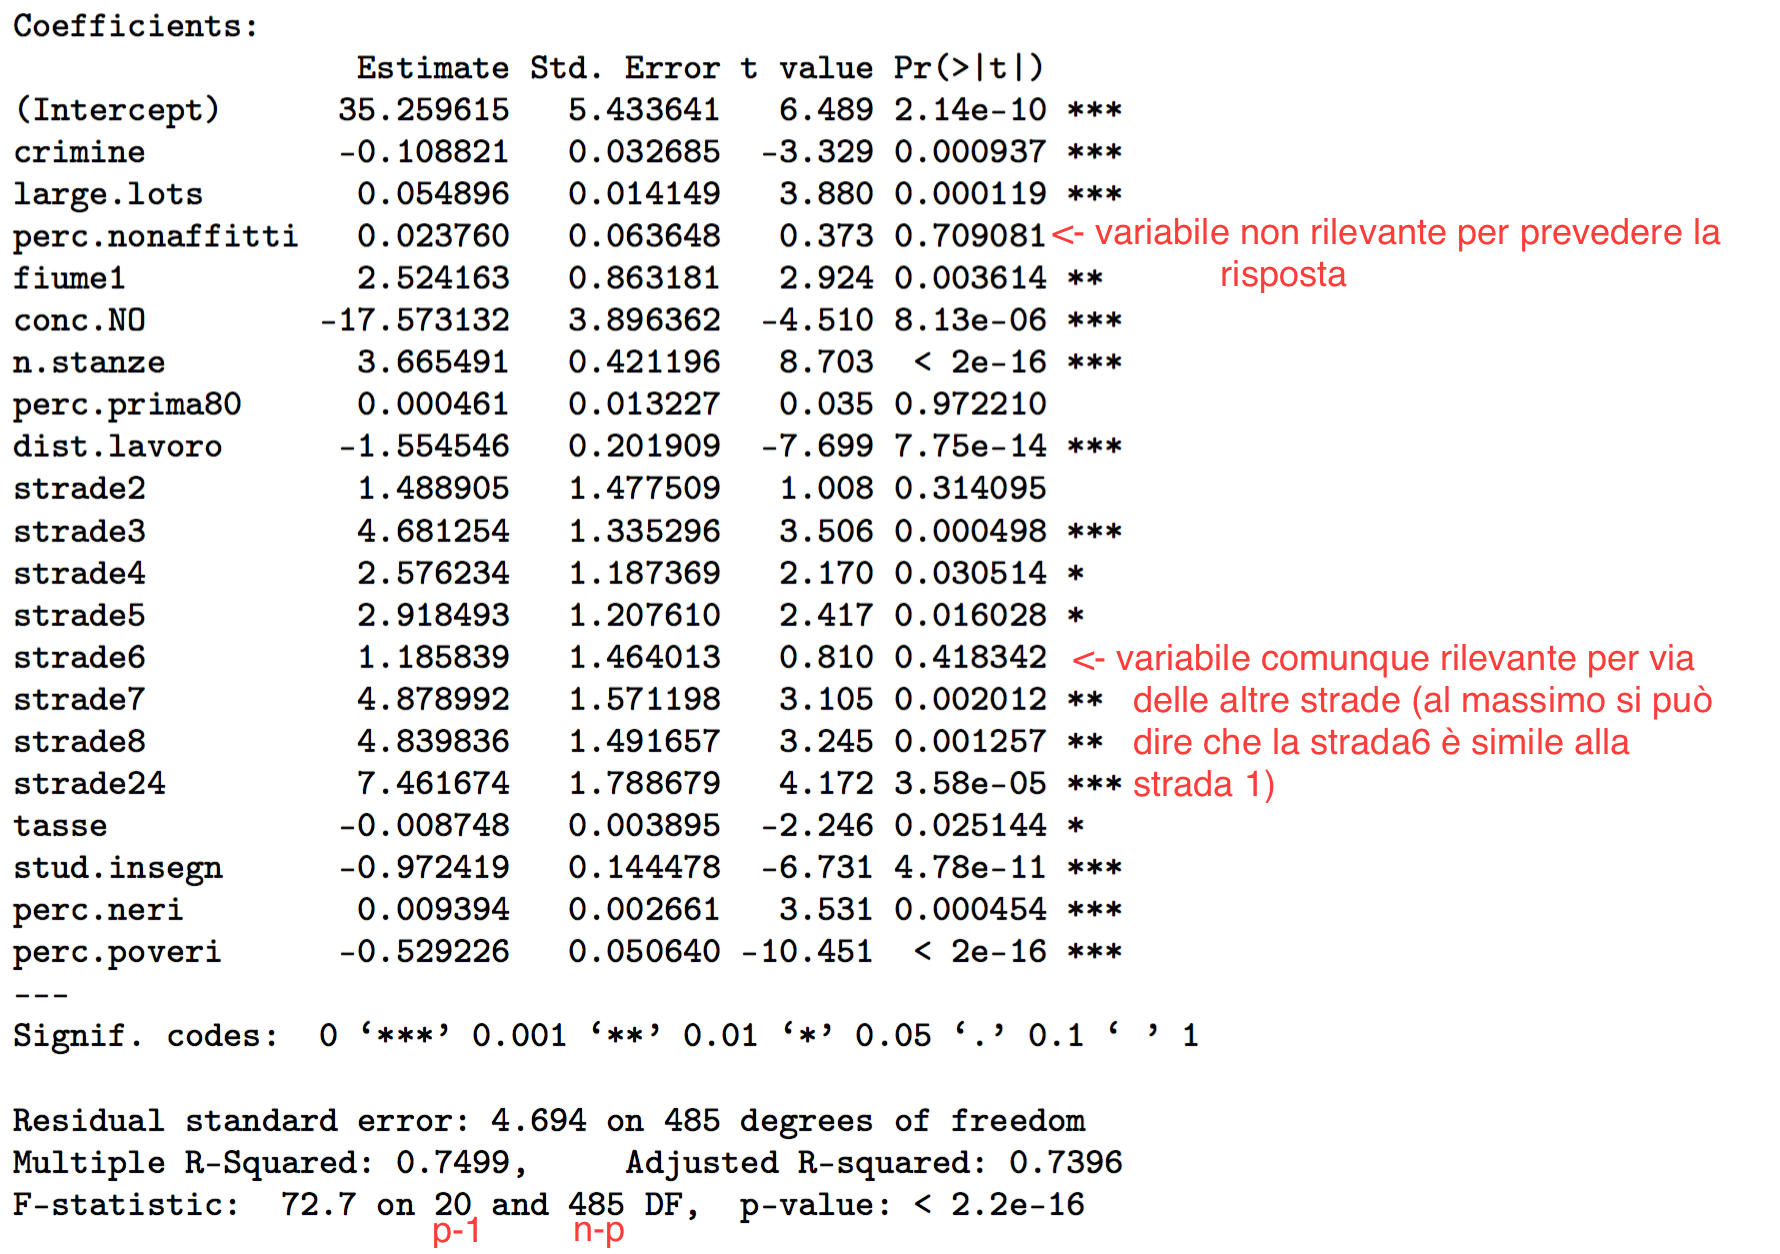
\includegraphics[width=.7\textwidth]{./notes/immagini/l10-fig1.png}
\end{figure}

\subparagraph{Dimostrazione}\label{dimostrazione-1}

Siano $ z_i $ e $ z_{i+p} $ dure caratteri di \textit{Z} a distanza \textit{p}. Siccome $ |\gamma|  \geq p$, i due caratteri possono essere appartenenti solamente o a \textit{X} o a \textit{Y} e mai ad entrambe le stringhe contemporaneamente. 
Pertanto dal momento che sia \textit{X} sia \textit{Y} hanno periodo \textit{p}, i due caratteri devono essere per forza uguali.

Da questo segue il lemma di periodicità che afferma che due periodi distinti \emph{p} e \emph{q} non possono coesistere troppo a lungo in
una stessa stringa senza che la stringa abbia anche periodo \emph{MCD(p,q)}.

\paragraph{Lemma - Lemma di periodicità}\label{lemma---lemma-di-periodicituxe0}

Sia \emph{X} una stringa di lunghezza \emph{n} con due periodi \emph{p}
e \emph{q} non entrambi nulli.

Se $n \geq p + q - MCD(p,q)$ allora la stringa \emph{X} ha anche periodo \emph{MCD(p,q)}.

\begin{figure}[htbp]
\centering
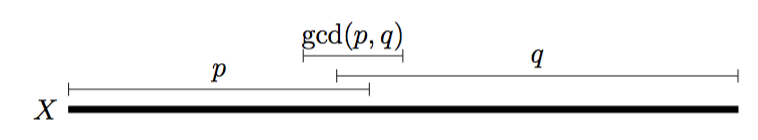
\includegraphics[width=.7\textwidth]{./notes/immagini/l10-fig2.png}
\caption{}
\end{figure}

\subparagraph{Dimostrazione}\label{dimostrazione-2}

Supponendo che $p \leq q$, la dimostrazione viene fatta per induzione su $p+q$.

$(p+q = 1)$ 

Se \emph{p=0} oppure \emph{p=q=0} allora \emph{MCD(p,q) = q} e dunque
\emph{X} ha periodo \emph{MCD(p,q)} perché ha periodo \emph{q}.

$(p+q > 1)$

Se \emph{p=0} o \emph{p=q} vale ancora il caso base.

Se $1 \leq p < q$, si ha che la stringa \emph{X} ha bordi $\alpha$ e $\beta$ di lunghezza \emph{n-p} e \emph{n-q}, questo per il primo lemma dimostrato.

\begin{figure}[htbp]
\centering
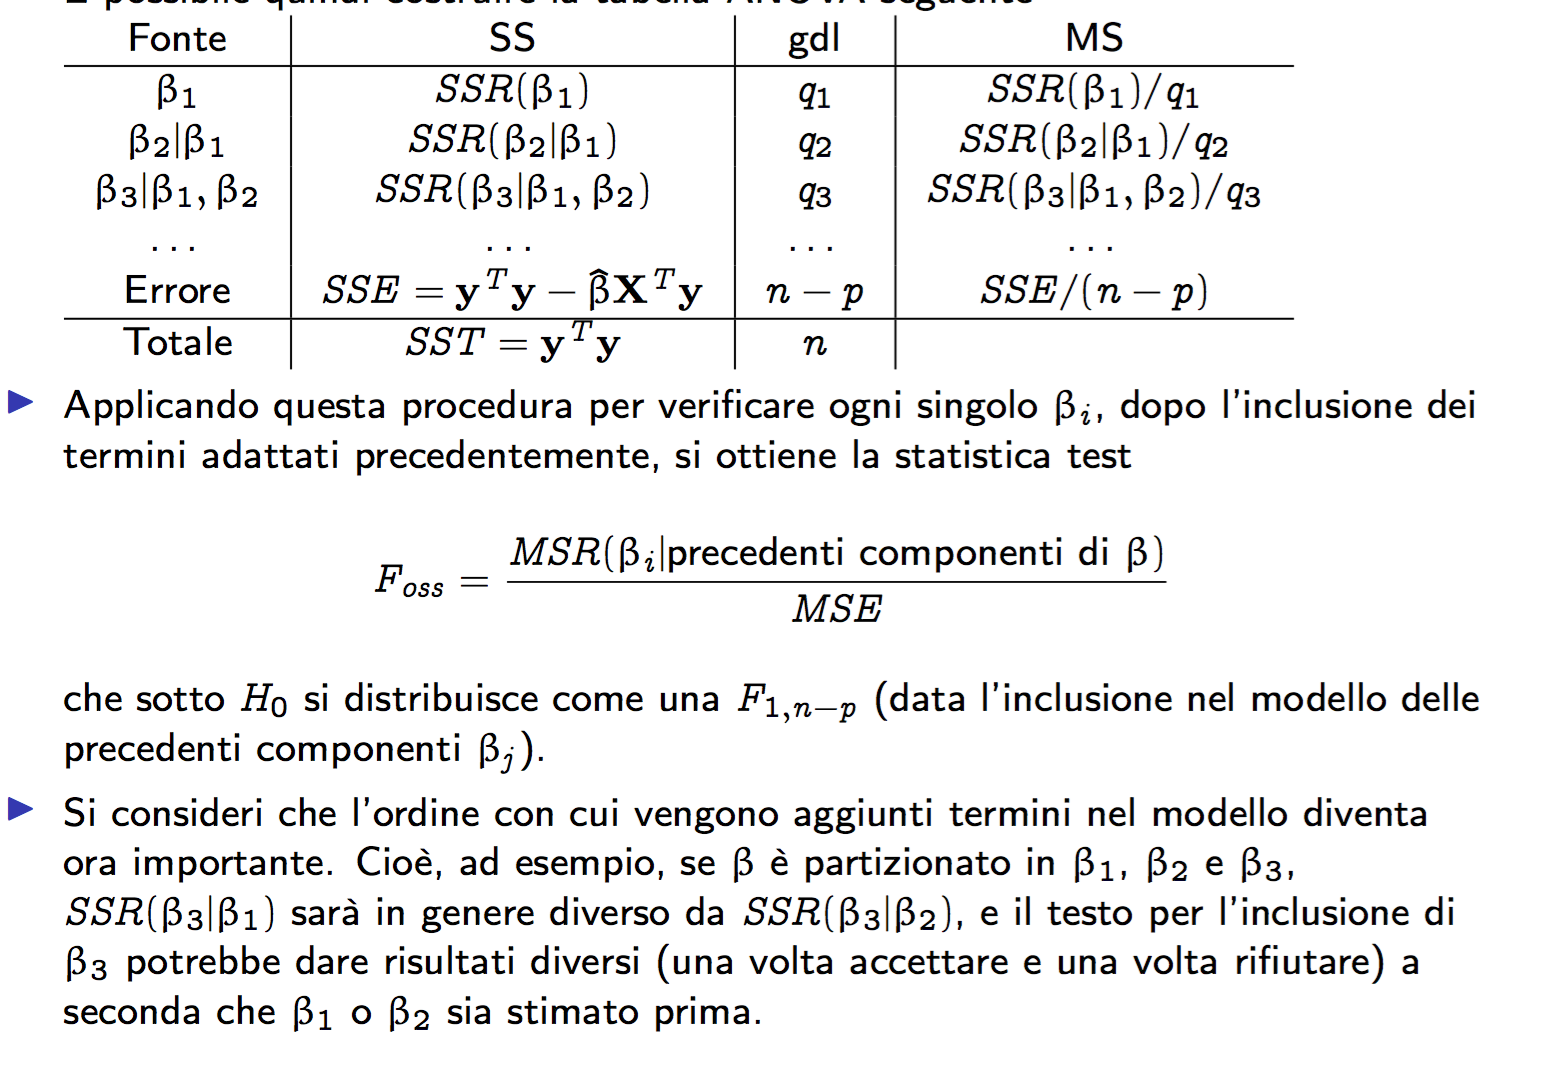
\includegraphics[width=.7\textwidth]{./notes/immagini/l10-fig3.png}
\caption{In verde la stringa $\alpha$ che si ripete con periodo
\emph{p}. In blu la stringa $\beta$ che si ripete con periodo
\emph{q}}
\end{figure}

La stringa $\beta$ essendo bordo di \emph{X} è anche bordo di $\alpha$ dal momento che $\alpha$ è un bordo di \emph{X}, pertanto $\alpha$ ha periodo $r = |\alpha| - |\beta| = q -p$.

Si ha che $p+r < p + q$, quindi è possibile applicare l'ipotesi induttiva, e che \emph{MCD(p,r) = MCD(p,q)}:

\begin{align*}
|\alpha| &\geq p+r-MCD(p,q)\\
 n - p &\geq q - MCD(p,q) 
\end{align*}

$ \alpha $ ha quindi come periodo sia \textit{r} (a causa di $ \beta $), sia \textit{p} (perché è una sottostringa di \textit{X}, la quale ha periodo \textit{p}) e per ipotesi induttiva ha anche periodo $MCD(p,r)$ che per come è definito \textit{r} è uguale a $MCD(p,q)$.

Considerando inoltre che:

\begin{align*}
	2|\alpha| &= (n-p) + (n-p) \\
					 &\geq q - MCD(p,q) + (n-p) \\
					 &\geq n
\end{align*}

perché $ p < q $ per ipotesi e $ MCD(p,q) \leq q - p $ per le proprietà del massimo comun divisore.

Questo implica che il prefisso $ \alpha $ di \textit{X} e il suffisso $ \alpha $ di \textit{X} coprono tutto \textit{X} e pertanto le due stringhe devono sovrapporsi\footnote{Non è possibile applicare il lemma della concatenazione perché non si sa di quanto queste stringhe si sovrappongono.} oppure $ X = \alpha\alpha $.

Presi quindi due caratteri $ x_i $ e $ x_j $ della stringa \textit{X}, tali che $ j - i = MCD(p,q) $ può succedere che i due caratteri appartengano alla stessa $ \alpha $ e quindi siano uguali, perché $ \alpha $ ha periodo $ r = MCD(p,q) $ oppure che $x_i \in \alpha_{(prefisso)} \text{ e } x_j \in \alpha_{(suffisso)} $.

\begin{figure}[htbp]
	\centering
	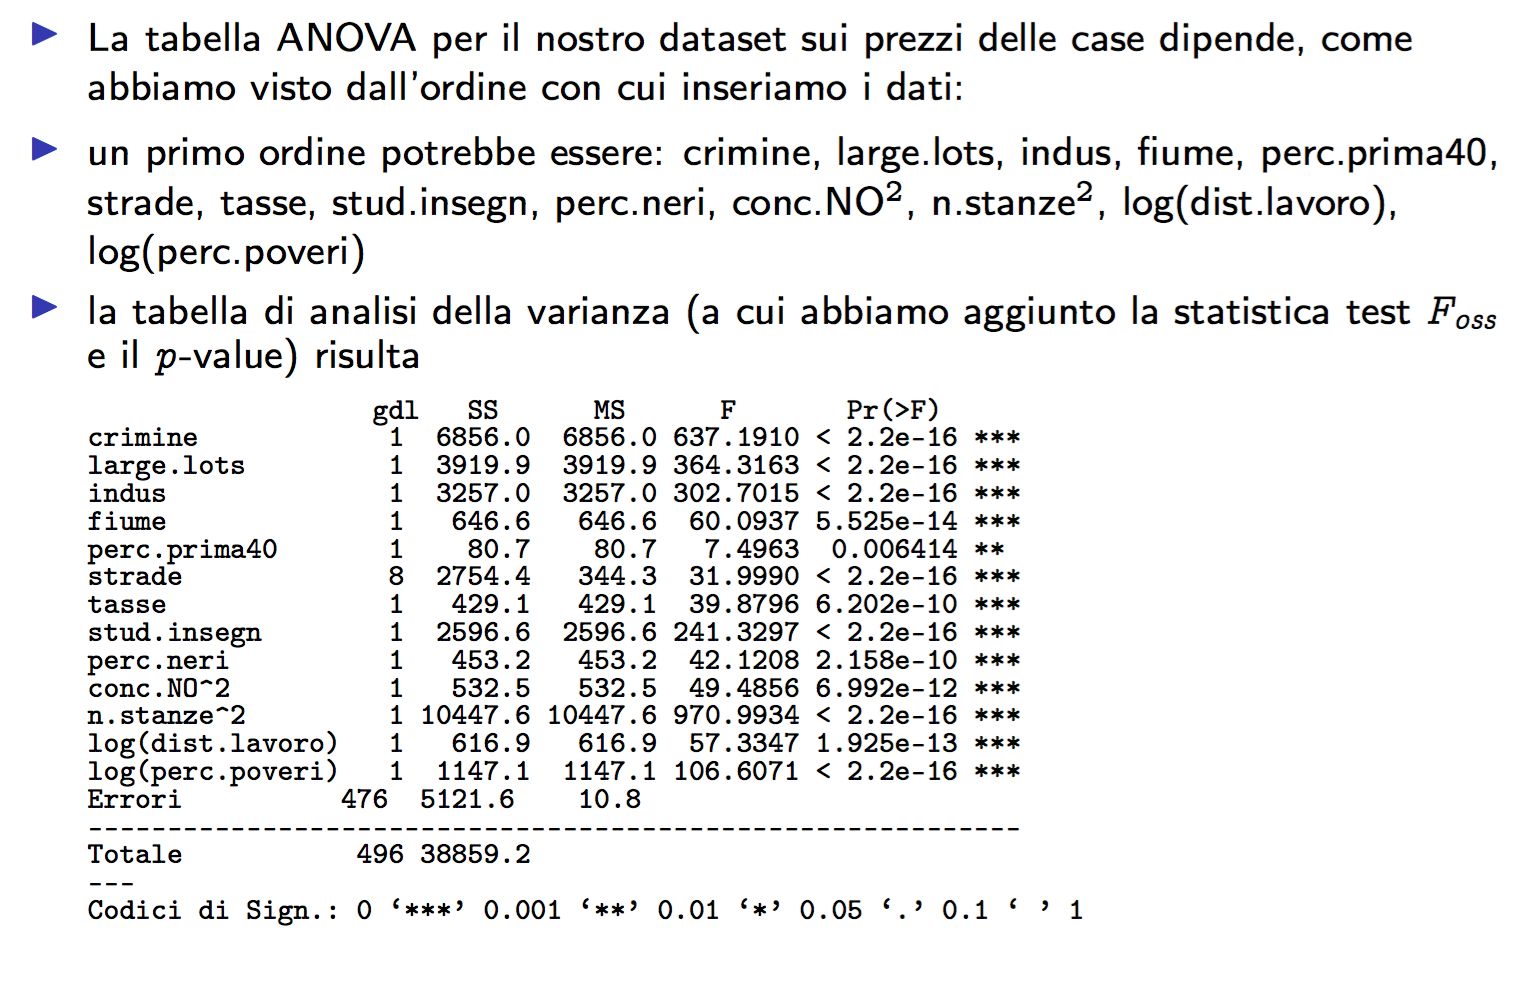
\includegraphics[width=.7\textwidth]{./notes/immagini/l10-fig4.png}
\end{figure}


In questo caso si ha che $ j > n - |\alpha| = p $ e quindi $ j - p \geq 1$. Si può quindi considerare il carattere $ x_{j-p} = x_j$ per via del periodo \textit{p} di $ X $ e che risulta appartenere a $ \alpha_{(prefisso)} $ perché $ p \geq MCD(p,q) $.

La distanza tra $ x_{j-p} \text{ e } x_i$ è $p - MCD(p,q)$, che per definizione è un multiplo di \textit{MCD(p,q)}, pertanto si ha che $ x_{j-p} \text{ e } x_i$ appartengono ad $ \alpha_{(prefisso)} $ che ha periodo \textit{MCD(p,q)}, pertanto $ x_{j-p} = x_i = x_j $ e di conseguenza \textit{X} ha periodo \textit{MCD(p,q)}.

	
	\textbf{Sottostringa}: serie di caratteri vicini

\textbf{Sottosequenza}: serie di caratteri non necessariamente vicini.

\section{Pattern matching di base}\label{pattern-matching-di-base}

Effettua il pattern matching esatto, cercando la sotto stringa \emph{P}
dentro la stringa \emph{T}.

\begin{breakablealgorithm}
	\caption{Ingenuo: Pattern matching ingenuo}
	\begin{algorithmic}[1]
	\Function{Ingenuo}{$ (P,T) $}
	\State $  $ \Comment{\textit{T} ha lunghezza \textit{n} e \textit{P} ha lunghezza $ m \leq n $}
	\For{$ i = 1 \: \text{to} n-m+1 $}
		\State $ j \gets 1 $
		\While{$ j \leq m \:\text{and} \:P[j] = T[i+j-1] $}
	        \State $ j \gets j + 1 $
	    \EndWhile
	    \If{$ j > m $}
	        \State Segnala l'occorrenza del pattern
	    \EndIf
	\EndFor
	\EndFunction
\end{algorithmic}
\end{breakablealgorithm}

\subsection{Utilizzo della sentinella}\label{utilizzo-della-sentinella}

La prima modifica che si può fare all'algoritmo per migliorarne
l'efficienza è quello di ridurre il test del \texttt{while}, rimuovendo
il controllo sulla lunghezza del pattern, riducendo così le operazioni
da 3 a 2.

Questo viene fatto aggiungendo una sentinella alla fine del pattern,
ovvero viene aggiunto al pattern un carattere che non compare
nell'alfabeto della stringa.

Perché questo funzioni è necessario aggiungere un carattere diverso
dalla sentinella anche alla fine di \emph{T} per permettere il match del
pattern anche quando questo è un suffisso della stringa.

\begin{breakablealgorithm}
	\caption{Ingenuo: Pattern matching ingenuo}
	\begin{algorithmic}[1]
		\Function{Ingenuo-2}{$ (P,T) $}
        \State //\textit{T} ha lunghezza \textit{n} e \textit{P} ha lunghezza $ m \leq n $
        \State $ P[m+1] \gets \$ $
        \State $ T[n+1] \gets @$
        \For{$ i = 1 \: \text{to } n-m+1 $}
	        \State $ j \gets 1 $
	        \While{$ P[j] = T[i+j-1] $}
		        \State $ j \gets j + 1 $
	        \EndWhile
	        \If{$ j > m $}
		        \State Segnala l'occorrenza del pattern
	        \EndIf
        \EndFor
        \EndFunction
\end{algorithmic}
\end{breakablealgorithm}

Nel caso non sia possibile modificare il testo si può togliere il
\texttt{+1} del ciclo \texttt{for} e sostituirlo con un \texttt{if} che
verifica l'uguaglianza dell'ultimo carattere.

D'ora in avanti assumeremo la presenza dei due caratteri sentinella.

\subsection{Riduzione del numero di confronti}\label{riduzione-del-numero-di-confronti}

Se il pattern contiene delle sottostringhe uguali, è possibile ridurre
il numero di controlli.

Ad esempio nel caso sotto riportato, l'algoritmo \textsc{Ingenuo}
effettua 20 confronti.

\begin{figure}[htbp]
\centering
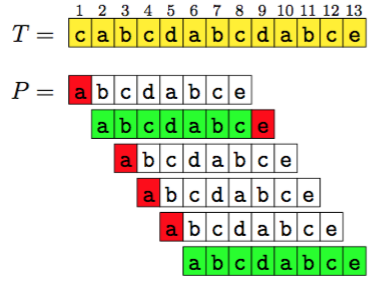
\includegraphics[width = .4\textwidth]{./notes/immagini/l11-fig1.png}
\end{figure}

Ovvero è possibile evitare il confronto tra l'inizio del pattern e il
terzo carattere del testo, perché si sa già che il terzo carattere del
testo è uguale al secondo carattere del pattern, il quale è diverso dal
primo carattere del pattern. Lo stesso ragionamento vale anche per i due
confronti successivi.

Ma si può fare di più, perché il pattern ha una sottostringa uguale al
suo prefisso, ovvero i caratteri 7-8-9 della del testo sono uguali ad
una sottostringa del pattern che coincide con il prefisso del pattern e
dal momento che questo è già questa uguaglianza è già stata verificata,
si possono ridurre ulteriormente i confronti.

\begin{figure}[htbp]
\centering
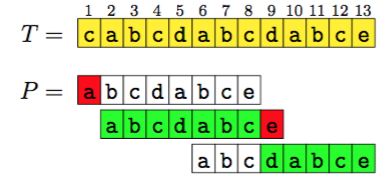
\includegraphics[width = .4\textwidth]{./notes/immagini/l11-fig2.png}
\end{figure}

Per poter applicare queste osservazioni ad un algoritmo è necessario
effettuare delle pre-elaborazioni delle stringhe.

\subsection{Pre-elaborazione fondamentale}\label{pre-elaborazione-fondamentale}

Data una stringa \emph{S} di lunghezza \emph{n}, la funzione
$\pi_i^S$ calcola la lunghezza del prefisso di \emph{S} più lungo
che occorre nella posizione \emph{i} di \emph{S}.

Quindi $\pi_i^S$ è il massimo \emph{h} tale che

$$
S[1,h] = S[i, i+h-1]
$$

Ad esempio:

\begin{figure}[htbp]
\centering
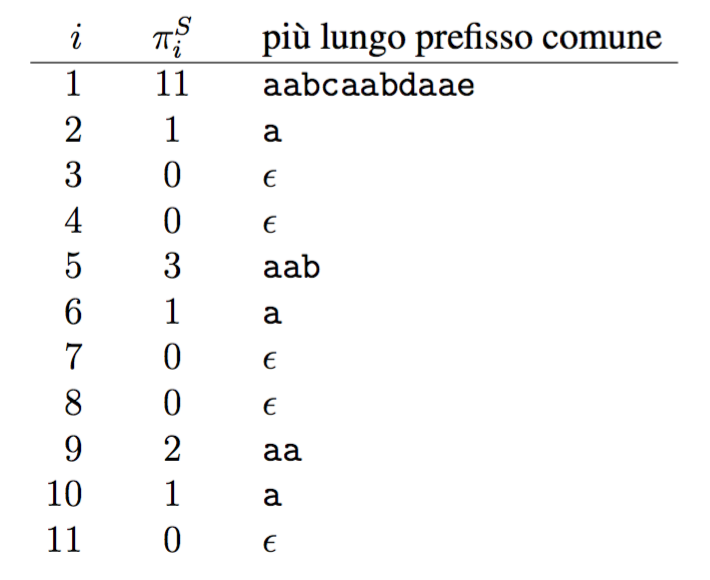
\includegraphics[width = .4\textwidth]{./notes/immagini/l11-fig3-bis.png}
\caption{$\pi_i$ per \textit{S=}\texttt{aabcaabdaae}.}
\end{figure}

Da notare che $Y = S[i, i+\pi_i -1]$ per definizione è un occorrenza in \textit{S} della stringa $S[1, \pi_i -1]$, pertanto si ha che \textit{Y} è un bordo della stringa $S[1, i +\pi_i -1]$. 
Per la relazione tra prefisso e bordo si ha quindi che $S[1, i +\pi_i -1]$ ha periodo $p = i -1$.

Si ha inoltre che la stringa $S[1, i +\pi_i -1]$ è il più lungo prefisso di \textit{S} con periodo $p= i-1$.

Questo perché se $i = 1$, si ha che il prefisso \textit{Y} coincide con \textit{S} e $p=0$, ottenendo periodo e bordo degeneri.

Se invece $ i \geq 2 $ si ha che, se $i + \pi_i -1 = n $, \textit{Y} è anche un suffisso di \textit{S}, pertanto non possono esserci altri prefissi con periodo $p = i -1$ più lunghi perché è la stringa \textit{S} è terminata.
Oppure se $i + \pi_i -1 \neq n $ vuol dire che il carattere $ S[\pi_i + 1] $ è diverso dal carattere $ S[i+\pi_i] $ per definizione di $ \pi_i $ e quindi non può esistere un prefisso $ S[1, \pi_i +1] $ con periodo $p = i -1$ perché $ S[\pi_i  + 1 + p] = S[\pi_i + i] $ che per ipotesi è diverso da $ S[\pi_i +1] $.

Le varie sottostringhe $ S[i, i + \pi_i -1 ] $ non sono necessariamente disgiunte ma possono sovrapporsi.

\subsubsection{Estremi massimi}

Fissato un $ i \geq 2 $, si ottengono varie stringhe $ S[j, j + \pi_j -1] $ con $ 2 \leq j \leq i $.

Tra tutte queste stringhe è possibile identificare la stringa che ha come valore dell' \textbf{estremo destro massimo}:

$$
r_i = \max \{ j + \pi_j -1 | \: 2 \leq j \leq i\}
$$

L'estremo sinistro associato viene indicato con 

$$
l_i = \arg\max\limits_{j} \{ j + \pi_j -1 | \: 2 \leq j \leq i\}
$$

Nel caso ci siano più sottostringhe con lo stesso estremo destro, viene scelto come estremo sinistro uno a caso tra quelli possibili.

La stringa $ S[l_i, r_i] $ risulta quindi essere la sottostringa di \textit{S} più lunga che è anche un prefisso e che inizia prima dell'indice \textit{i}.

\begin{figure}[htbp]
	\centering
	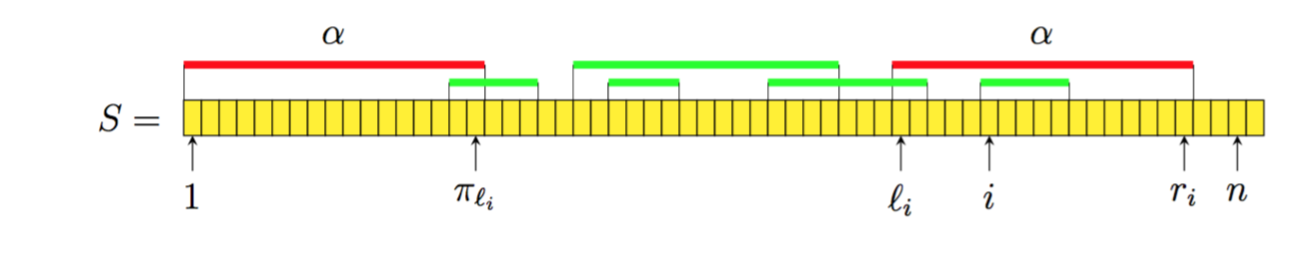
\includegraphics[width = .9\textwidth]{./notes/immagini/l11-fig4-bis.png}
	\caption{Alcune occorrenze di prefissi di \textit{S} che iniziano tra le posizioni \textit{2} e \textit{i}. L'occorrenza che termina più a destra è evidenziata in rosso.}
\end{figure}

Si ha quindi che $ S[1,r_i] $ è il più lungo prefisso di \textit{S} con periodo $ 1 \leq p < i $ e che la stringa $ S[l_i, r_i] $ è la sottostringa di \textit{S} che termina più a destra tra tutte quelle che sono uguali ad un prefisso di \textit{S}.

Ad esempio se 

$$
S = \text{\texttt{aabaabcadaabaabce}}
$$

il massimo destro con $ 2 \leq j \leq 15 $ è $ r_{15} = 10 + \pi_{10} -1 = 16$, perché $ \pi_{10} = 7$, e $ l_{15} = 10 $ che è la posizione in cui inizia la sottostringa \texttt{aabaabc}.

\subsection{Pre-elaborazione fondamentale in tempo lineare}\label{preambolazione-fondamentale-in-tempo-lineare}

Seguendo l'approccio di definizione il tempo richiesto è
$O(n^2)$, ma è possibile scendere a $O(n)$.

Supponiamo che \emph{S} termini con un carattere diverso da tutti gli
altri che compaiono nella stringa. Questo non è un problema perché si
può sempre aggiungere una sentinella.

L'algoritmo calcola $\pi_1 = n$ e poi calcola i valori $\pi_i, r_i, l_i$ per $i = 2,\ldots, n$, basandosi su un'array $ pref[1\ldots n] $ il quale conterrà i vari $ \pi_i $ e due variabili, \textit{r} e \textit{l}, le quali andranno a memorizzare gli estremi massimi tra gli indici precedente calcolati.

Come prima cosa viene effettuato il calcolo di $ \pi_2 $ confrontando da sinistra a destra i caratteri di $S[2,n]$, cosi facendo si ha che $ r = \pi_2 +1 $ e $l = 2$.

Assumendo induttivamente di aver calcolato $ \pi_j $ per ogni $ j = 2, \ldots, i-1$, si ha che $ r = r_{i-1} = \pi_{i-1} +1 $ e $ l = l_{i-1} $.

Durante il calcolo di $ \pi_i $ possono verificarsi 2 casi:

\begin{enumerate}
	\item $ i > r $: non si hanno informazioni riguardo ai caratteri che seguono \textit{i}, quindi viene effettuato il calcolo di $ \pi_i $ normalmente, andando ad effettuare i confronti da sinistra a destra tra $ S[i,n] $ e \textit{S}. Il valore di $ \pi_i $ è allora uguale alla lunghezza \textit{h} del massimo prefisso comune e $ r = i  + \pi_i +1 $ e $ l= i $.
	\item $ i \leq r$: il carattere \textit{S[i]} è contenuto nella sottostringa $ \alpha = S[l,r] $ la quale è anche prefisso di \textit{S}. Si ha quindi che il carattere \textit{S[i]} compare anche nella posizione $ i' = i - l +1 $ di \textit{S} e per lo stesso motivo la stringa $ \beta = S[i,r] $ compare anche in $ S[i', \pi_l] $.
	\begin{figure}[htbp]
		\centering
		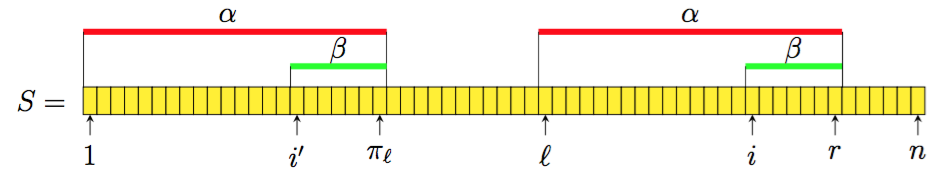
\includegraphics[width = .8\textwidth]{./notes/immagini/l11-fig3.png}
	\end{figure}
	In \textit{i'} occorrerà un prefisso $ \gamma $ di \textit{S} di lunghezza $ \pi_{i'} $, che può anche essere degenere.
	Questo prefisso occorrerà a partire dalle posizioni \textit{1} e \textit{i'} e potrà essere contenuto o contenere la sottostringa $ \beta $.
	Ne segue che \textit{S} e \textit{S[i,n]} hanno un prefisso in comune di lunghezza uguale al minimo tra $ \pi_{i'} $ e $ |\beta| = r - i +1 $.
	\begin{enumerate}
		\item $ \pi_{i'} < |\beta| $: il prefisso che inizia in \textit{i} ha la stessa lunghezza di quello che inizia in \textit{i'}, ed avendo già calcolato la lunghezza di quel prefisso si ha che $ \pi_i = \pi_{i'} $ senza effettuare alcun confronto.
		\begin{figure}[htbp]
			\centering
			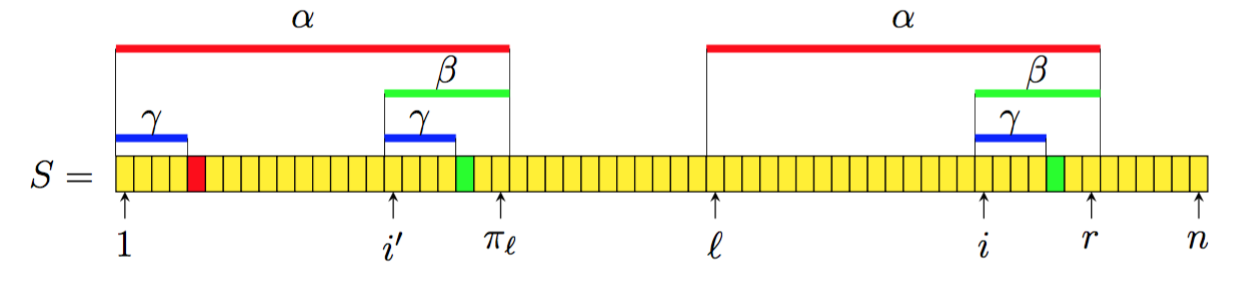
\includegraphics[width = .8\textwidth]{./notes/immagini/l11-fig5.png}
		\end{figure}
		\item $ \pi_{i'} \geq |\beta|$: l'intera sottostringa $ \beta = S[i,r] $ deve essere un prefisso di \textit{S} e quindi $\pi_i \geq |\beta| = r - i +1$. L'algoritmo calcola quindi la lunghezza \textit{h} del massimo prefisso comune tra \textit{S} e \textit{S[i,n]} a partire dai caratteri $ |\beta| + 1 $ e $ i + |\beta| $, fino a che non trova un mismatch. A questo punto vengono posti $ \pi_i =h,\: r= i + \pi_i -i \: \text{e} \: l = i $.
	\end{enumerate}
	
\end{enumerate}

\begin{breakablealgorithm}
	\caption{Prefisso: Preelaborazione del prefisso in tempo lineare}
	\begin{algorithmic}[1]
		\Function{Prefisso}{$ S $}
		    \State // S stringa di lunghezza n > 1 con sentinella alla fine
		    \State $ pref[1] \gets n $  \Comment{$ \pi_i, \pi_1 = n$}
		    \State $ h \gets 0 $
		    \While{$ S[1+h] = S[2+h] $}\Comment{Calcola $\pi_2$}
		        \State $ h = h +1 $
		    \EndWhile
		    \State $ pref[2] \gets h $
		    \State  $ l \gets 2 $
		    \State $ r \gets 2 + h - 1$
		    \For{$ i = 3 \: \text{to} \: n $}
			    \If{$ r < i $} \Comment{Caso 1}
			        \State $ h \gets 0$
		            \While{$ S[1+h] = S[i+h]$}
		                \State $ h \gets h + 1 $
		            \EndWhile
		            \State $ pref[i] \gets h$
		            \State $ l \gets i $
		            \State $ r \gets i + h -1 $
		        \Else \Comment{Caso 2}
				    \If{$pref[i-l+1] < r - i +1$} \Comment{Caso 2a}
		                \State $pref[i] \gets pref[i - l +1]$
		            \Else \Comment{Caso 2b}
		               \State $h \gets r - i +1$
		                \While{$S[1+h] = S[i +h]$}
		                    \State $ h \gets h +1 $
		                \EndWhile
		                \State $pref[i] \gets h$
		                \State $l \gets i$
		                \State $ r \gets i +h -i$
			         \EndIf
		          \EndIf
		    \EndFor
		    \State \Return $ pref $
		   \EndFunction
	\end{algorithmic}
\end{breakablealgorithm}

La correttezza dell'algoritmo deriva da quanto detto prima

\paragraph{Complessità}\label{complessituxe0}

Se non viene presa in considerazione la complessità dei cicli
\texttt{while} si ha che la complessità è data da \emph{O(n)}.

I cicli \texttt{while} terminano quando viene trovato un mismatch e al
massimo vengono trovati \emph{n-1} mismatch (1 dal \texttt{while}
esterno, $n-2$ dai \texttt{while} dentro il ciclo \texttt{for}).

Ad ogni confronto con successo, il carattere destro ($S[i+h]$)
viene spostato a destra di 1 e, una volta terminato il \texttt{while}, questo viene posto a $r = i + h - 1$, ovvero risulta essere il carattere alla posizione $S[r+1]$.

All'iterazione successiva il ciclo \texttt{while} inizia con carattere destro $S[i]$ se $i > r$\footnote{Viene quindi sposto a destra perché $ i \geq r+1 $} altrimenti inizia con $S[i + h]$ con $h = r - i + 1$. In entrambi i casi il carattere destro non si sposta mai a sinistra durante l'esecuzione dell'algoritmo. 
Pertanto vengono eseguiti al più $n-1$ confronti con successo. +
Si ottiene quindi una complessità per i \texttt{while} di $O(2n-2)$.

La complessità totale dell'algoritmo è data da $O(n) +\textit{ Complessità while }= O(n) + O(2n-2) = O(n)$.

\subsubsection{Matching esatto in tempo lineare}\label{matching-esatto-in-tempo-lineare}

Per effettuare il pattern matching in tempo $O(m+n)$ del pattern \emph{P} in \emph{T} è possibile utilizzare una versione leggermente modifica della funzione prefisso sulla stringa \emph{S = P\$T}, dove \$ è un simbolo che non è presente nelle due stringhe.

Questo viene fatto calcolando $ \pi_i^S $ per $ i = 2, \ldots n + m +1 $.
Siccome \$ non compare in nessuna delle due stringhe, si ha che $ \pi_i \leq m \: \forall \: i $ perché per ipotesi la sottostringa \textit{P\$} non può comparire all'interno di \textit{T}.
Inoltre, $ \forall \: i \geq m +1 : \pi_i = m $ si ha che $i - m - 1$ identifica l'inizio di un'occorrenza di \textit{P} in \textit{T}, perché $ \pi_i = m $ indica la presenza di prefisso di lunghezza \textit{m} a partire dalla posizione \textit{i}, ma la sottostringa prefissa di lunghezza \textit{m} coincide per costruzione con \textit{P}, quindi \textit{i} indica l'inizio di un'occorrenza del pattern \textit{P} nella stringa \textit{P\$T}.

Dal momento che il prefisso viene calcolato in tempo lineare rispetto la lunghezza della stringa, si ottiene una funzione di pattern matching con complessità lineare.

Altre caratteristiche di questo algoritmo sono:
\begin{itemize}
	\item il \textbf{consumo lineare di memoria} rispetto la lunghezza del pattern $ O(m) $, perché è possibile evitare di tenere in memoria tutti $ \pi_i $ con $ i >m $ perché tutti i valori \textit{i'} del caso 2 faranno sempre riferimento ai $ \pi_i \: \text{con}\: i \leq m $
	\item che non è necessario conoscere tutto l'alfabeto, basta avere la possibilità di confrontare i caratteri.
\end{itemize}

\subsubsection{Esercizio - Identificare una rotazione}

Date due stringhe \textit{X} ed \textit{Y} di uguale lunghezza \textit{n}, determinare in tempo lineare \textit{O(n)}, se \textit{Y} è una rotazione circolare di \textit{X}.
Ovvero se è possibile identificare due stringhe $ \alpha $ e $ \beta $ tali che $ X = \alpha\beta $ e $ Y = \beta\alpha $.

\paragraph{Soluzione}

Si concatenano le stringhe in modo da formare $ S = Y\$XX $, se eseguendo la preelaborazione trovo un prefisso di lunghezza \textit{n} a partire dal $n+1$ vuol dire che \textit{Y} compare tra le due \textit{X} e quindi le due stringhe sono la rotazione di una stessa stringa.

\subsubsection{Esercizio - Massima sottostringa comune}

Date due stringhe \textit{X} e \textit{Y} di lunghezza \textit{m} e \textit{n} calcolare, in tempo lineare, il più lungo suffisso di \textit{X} che è anche prefisso di \textit{Y}. 
Ovvero la sottostringa $ \gamma $ di lunghezza massima tale che $ X = \alpha\gamma \: \text{e} \: Y = \gamma\alpha$.

\paragraph{Soluzione}

L'idea è quella di concatenare due stringhe in modo da formare $ S= Y\$X $, dove \$ è un carattere che non compare in nessuna delle due stringhe, per poi effettuare la preelaborazione.

Se $ \pi_2^S = 0$ non c'è nessuna sottostringa uguale al prefisso di \textit{Y}, quindi $ \gamma = \epsilon $, altrimenti se  $ 0 < \pi_2^S = k \leq m$ si ha che c'è un'occorrenza all'interno di \textit{S} del prefisso di \textit{Y} lunga \textit{k}, ma non si ha alcuna garanzia che questa sia un suffisso per \textit{X}.

Se  $ \pi_{n+m+1-k}^S = k$ si ha che a partire dal carattere $ n+m+1-k $ c'è un match di una sottostringa di lunghezza \textit{k} che per costruzione è anche suffisso di \textit{X}, pertanto $ \gamma = Y[1,k] $, altrimenti la sottostringa precedentemente identifica si trova o all'interno di \textit{Y} o all'interno di \textit{X}, pertanto $ \gamma = \epsilon $.

\todo[inline]{Quasi corretto, bisogna andare a vedere i $ \pi_j $ per trovare il suffisso più lungo che è anche prefisso.}



	% !TEX encoding = UTF-8
% !TEX TS-program = pdflatex
% !TEX root = computabilità e algoritmi.tex
% !TEX spellcheck = it-IT
\paragraph{Soluzione}\label{soluzione-esercizio}

La funzione \emph{f(x)} viene definita per casi e dal momento che i vari
predicati sono decidibili ed esaustivi, quindi almeno uno dei casi è
vero.

$$
f(\vec{x}) = f_1(\vec{x}))\cdot \mathcal{X}_{Q_1} + \ldots +	 f_m(\vec{x}))\cdot \mathcal{X}_{Q_m}
$$

Quando un caso è vero, viene calcolata la funzione associata, che è
totale. Se questa funzione non fosse totale, potrebbe essere che il
predicato vero su un certo \emph{x}, ma che la funzione su
quell'\emph{x} non sia definita e quindi neanche \emph{f(x)}
risulterebbe definita, perdendo così la totalità.

La calcolabilità deriva dal fatto che la definizione per casi viene
fatta con una serie di \emph{if} che è dimostrato essere calcolabile e
le funzioni $\mathcal{X}_{Q_i}$ sono calcolabili, perché i predicati sono
decidibili.

\subsubsection{Algebra della decidibilità}\label{algebra-della-decibilituxe0}

I predicati decidibili sono chiusi rispetto negazione, congiunzione e
disgiunzione.

Ovvero se \textit{Q} e \textit{Q'} sono due predicati in $\mathbb{N}^k$ decidibili allora anche:

\begin{enumerate}
\item $\neg Q(\vec(x))$
\item $ Q(\vec{x}) \wedge Q'(\vec{x})$
\item $ Q(\vec{x}) \vee Q'(\vec{x}) $
\end{enumerate}

Questo perché le relative funzioni che li calcolano possono essere definite come:

\begin{enumerate}
	\item $ \mathcal{X_{\neg Q}}(\vec{x}) = \overline{sg}( \mathcal{X_{Q}}(\vec{x})) $
	\item $ \mathcal{X_{Q \wedge Q'}}(\vec{x})= \mathcal{X_{Q}}(\vec{x}) \cdot \mathcal{X_{Q'}}(\vec{x})$
	\item $ \mathcal{X_{Q \vee Q'}}(\vec{x})= sg(\mathcal{X_{Q}}(\vec{x}) + \mathcal{X_{Q'}}(\vec{x}))$
\end{enumerate}

Tutte le funzioni così definite sono calcolabili perché ottenute da composizioni di funzioni calcolabili.

\subsubsection{Somma e prodotto dei valori di una funzione}

Data una funzione totale e $ f : \mathbb{N}^{k+1} \rightarrow  \mathbb{N}$ totale e calcolabile, è possibile definire le due funzioni che effettuano la somma e il prodotto dei primi \textit{y} valori della funzione.

\begin{align*}
	s(\vec{x}, y) &= \sum_{z < y} f(\vec{x},z) \\
	p(\vec{x}, y) &= \prod_{z < y} f(\vec{x},z) 
\end{align*}

Entrambe le funzioni sono calcolabili e totali perché possono essere definite induttivamente (ricorsivamente) a partire da delle funzioni calcolabili.

\begin{align*}
s(\vec{x}, y) &= \begin{cases} \sum_{z < 0}f(\vec{x},z) = 0, &\text{ se $ y = 0 $} \\
\sum_{z < y+1}f(\vec{x},z) = \sum_{z < y}f(\vec{x},z) + f(\vec{x},z), &\text{ altrimenti}
\end{cases} \\
p(\vec{x}, y) &=  \begin{cases} \prod_{z < 0}f(\vec{x},z) = 1, &\text{ se $ y = 0 $} \\
\prod_{z < y+1}f(\vec{x},z) = \prod_{z < y}f(\vec{x},z) \cdot f(\vec{x},z) &\text{ altrimenti}
\end{cases}
\end{align*}

La totalità deriva dal fatto che \textit{f} è totale.

\subsubsection{Quantificazione limitata}

Combinando algebra della decidibilità e quanto detto nel paragrafo precedente è possibile la decidibilità di $ \forall $ e $ \exists $.

Dato un predicato $ Q(\vec{x},z) $ per calcolare se $ \forall z < y, Q(\vec{x},z) $ è possibile utilizzare la funzione:

$$
\mathcal{X}_{Q_\forall} = \prod_{z < y} \mathcal{X}_Q(\vec{x},z)
$$

In modo simile è possibile calcolare $ \exists z < y, Q(\vec{x},z) $:

$$
\mathcal{X}_{Q_\exists} = sg(\sum_{z < y} \mathcal{X}_Q(\vec{x},z))
$$

Trattandosi della composizione di funzioni calcolabili e totali, le funzioni così ottenute sono a loro volta calcolabili e totali.

\section{Minimalizzazione limitata}

Data una funzione $ f(\vec{x},z) : \mathbb{N}^{k+1} \rightarrow \mathbb{N}$ calcolabile e totale è possibile definire una funzione 

$$
h(\vec{x},y) = \mu z< y | f(\vec{x},z) = 0
$$

$ h $ è ancora una funzione $ \mathbb{N}^{k+1} \rightarrow \mathbb{N} $ e viene calcolata come il minimo valore di \textit{z} minore di \textit{y} e tale che $ f(\vec{x},z) $ sia uguale a 0 (tipicamente l'uguale a 0 viene omesso). 

La definizione più precisa è:

$$
h(\vec{x}, y) = \mu z < y . f(\vec{x},z) = \begin{cases}
\text{minimo $ z < y $ tale che $f(\vec{x},z) = 0$ se questo esiste} \\
y, \text{altrimenti}
\end{cases}
$$

Per come è definita, questa funzione risulta essere \textbf{totale} e \textbf{calcolabile}.
Intuitivamente è calcolabile perché si tratta di calcolare \textit{f} per vari valori, serve però una dimostrazione più formale, fatta per ricorsione primitiva.

\begin{align*}
	h(\vec{x}, 0) &= 0\\
	h(\vec{x}, y+1) &= 	\begin{cases}
										h(\vec{x},y) < y, &\text{\textit{f} si annulla su un valore minore di \textit{y}, viene resituito $ h(\vec{x},y) $}\\
										h(\vec{x},y) = y, &\text{per tutti i valori di minori \textit{y} non c'è uno 0 } \begin{cases}
										\text{se } f(\vec{x},y) = 0 \rightarrow y \\ 
										\text{se } f(\vec{x},y) \neq 0 \rightarrow y+1
										\end{cases}
										\end{cases}
\end{align*}

La seconda parte può essere facilmente tradotta nell'espressione

$$
(y \dotminus h(\vec{x},y)) \cdot (h(\vec{x},y)) + \overline{sg}(y \dotminus h(\vec{x},y)) \cdot (y + sg(f(\vec{x},y)))
$$

Dal momento che la funzione \textit{h} può essere definita per ricorsione primitiva e per composizione di funzioni calcolabili, anche lei è calcolabile.

\subsection{Funzioni calcolabili per ricorsione limitata}

Utilizzando la ricorsione limitata è possibile dimostrare la calcolabilità di varie funzioni.

\subsubsection{Numero di divisori di $x$}

\begin{align*}
	D(x) &= \text{\# divisori di } x \\
			&= \sum_{y \leq x}(\overline{sg}(rm(y,x))) 
\end{align*}

Dove \textit{rm} è la funzione resto, precedentemente dimostrata calcolabile.

\subsubsection{Numeri primi}

Dimostrare la calcolabilità dei funzioni che lavorano con i numeri primi è importante perché torneranno utili in futuro.

\begin{align*}
	Pr(x) &= \text{``$x$ è primo ''} \\
			 &= \overline{sg}(|D(x) - 2|)
\end{align*}

\begin{align*}
	P_x &= \text{``$x$-esimo numero primo, per convezione: ''} P_0 = 0, P_1 = 2, \ldots \\
	&= \begin{cases}
	P_0 = 0& \\
	P_{x+1} = \mu z \leq (P_x! + 1) \: | Pr(z) \cdot \underbrace{\overline{sg}(P_x +1 \dotminus z)}_{1 \text{ se } z > P_x  } \dotminus 1| &
	\end{cases}
\end{align*}

\begin{align*}
	(x)_y 	&= \text{esponente di  } P_y \text{ nella decomposizione di } y \\
			   &= \text{max } z \: P_{y}^z \text{ divide } x \rightarrow \mu z \leq x \text{ tale che } P_{y}^{z+1} \text{ non divide } x \\
			   &= \mu z \leq x \: \overline{sg}(rm(P_{y}^{z+1},x))
\end{align*}

\subsubsection{Esercizio - mcm, MCD, radice di x}

Dimostrare che sono calcolabili:

\begin{itemize}
	\item $ floor(\sqrt{x}) $
	\item $mcm(x,y))$
	\item $MCD(x,y)$
\end{itemize}


\section{Codifica di coppie}

La funzione di \textit{fibonacci} non può essere definita per ricorsione primitiva, perché il passo induttivo richiede una coppia di valori precedenti.

\`{E} però possibile definire una funzione $\prod : \mathbb{N} \times \mathbb{N} \rightarrow \mathbb{N}$ che codifica il valore di una coppia in un unico numero:

$$
\prod (x,y) = 2^x(2y+1) \dotminus 1
$$

Questa funzione risulta essere biunivoca perché è possibile definire l'inversa:

$$
\prod^{-1}(x) = ((n+1)_1, \frac{1}{2}(\frac{n+1}{(n+1)_1})-1)
$$

La funzione inversa è effettiva, perché è definita in termini di componenti calcolabili, anche se la definizione di funzione calcolabile non è stata vista per funzioni $\mathbb{N} \rightarrow \mathbb{N} \times \mathbb{N}$.

Utilizzando la funzione accoppiamento, è possibile definire la funzione \textit{fib} per ricorsione primitiva:

\begin{align*}
	g(x) &= \prod(fib(x), fib(x+1)) \\
	g(0) &= \prod(fib(0), fib(1)) = \prod(1,1) = 5 \\
	g(x+1) &= \prod(fib(x+1), fib(x+2)) \\
				 &= \prod(fib(x+1, fib(x)+fib(x+1)) \\
				 &= \prod(\prod_2(g(x)),\prod(\prod_1(g(x))+\prod_2(g(x)))\\		 
\end{align*}

Dove $\prod_1$ e $\prod_2$ sono rispettivamente le funzioni per il calcolo del primo e del secondo elemento della coppia.

Così facendo è stata dimostrata la calcolabilità di \textit{g} per ricorsione primitiva, ma $fib(x) = \prod_1(g(x))$ e di conseguenza \textit{fib} è calcolabile per composizione di funzioni calcolabili.

\section{Minimalizzazione illimtata}

Data $ f : \mathbb{N}^{k+1} \rightarrow \mathbb{N} $, si vuole definire $ h : \mathbb{N}^k \rightarrow \mathbb{N} $ tale che calcoli il minimo \textit{z} che azzera la funzione \textit{f}, ovvero:

$$
h(\vec{x}) = \mu z.f(\vec{x},z)
$$

Ci sono però dei problemi se $ f(\vec{x}, z) $ è sempre diversa da zero, perché in questo caso $ h $ è $ \uparrow $.

Un altro problema si ha se la funzione è indefinita per un valore $ z' $ minore dello $ z $ che azzera la funzione. Anche in questo caso si ha che $ h $ è $ \uparrow $.

$$
h(\vec{x}) = \mu z.f(\vec{x},z) = \begin{cases}
\text{minimo \textit{z} tale che } f(\vec{x},z) = 0 \text{ se esiste e se } \forall z' < z, f(\vec{x},z')\downarrow \neq 0 \\
\uparrow \text{ altrimenti}
\end{cases}
$$

Alternativamente, definendo $ Z_{f, \vec{x}} = \{z | f(\vec{x},z) = 0 \wedge \forall z' < z f(\vec{x},z') \downarrow \} $, si ha che \textit{h} è definita come

$$
h(\vec{x}) = \begin{cases}
\min Z_{f,\vec{x}} \text{ se } Z_{f,\vec{x}} \neq \emptyset \\
\uparrow \text{ altrimenti}
\end{cases}
$$

\subsection{Esercizi}

\subsubsection{Esercizio - Radice quadrata}
Dimostrare la calcolabilità di 

$$
f(x) = \begin{cases}
\sqrt{x} \text{ se \textit{x} è un quadrato} \\
\uparrow \text{ altrimenti}
\end{cases}
$$

\paragraph{Soluzione}

L'idea è quella di trovare un \textit{y} che elevato al quadrato è uguale a \textit{x}: $ y^2 - x = 0 $.

Si ha quindi che

$$ 
f(x) = \mu y.|y^2-x|
$$

ed è calcolabile perché minimizza illimitatamente una composizione di funzione calcolabile.

\subsubsection{Esercizio teorico}

Dimostrare che se $ f : \mathbb{N} \rightarrow \mathbb{N} $ è iniettiva, calcolabile e totale, anche la sua inversa è calcolabile.

\paragraph{Soluzione}

$$
f^{-1}(x) = \begin{cases}
y, &\text{ tale che } f(y) = x \\
\uparrow, &\text{ altrimenti}  
\end{cases}
$$

$$ 
f^{-1}(x) = \mu y.|f(y)-x|
$$

Perché l'uguaglianza sia rispettata è necessario che \textit{f} sia totale, dal momento che se per un certo \textit{y}, \textit{f} non è definita il programma che la calcola non termina, rendendo indefinita anche $ f^{-1} $.

C'è un barbatrucco per gestire anche la non totalità di \textit{f}, ovvero quello di eseguire contemporaneamente il calcolo per ogni \textit{y}, eseguendo tot passi alla volta per ognuno dei calcoli (\textit{dovrebbe essere dimostrato in futuro}).

Dal momento che \textit{f} è calcolabile si ha che anche l'inversa è calcolabile per minimizzazione illimitata di una composizione di funzioni calcolabili.

L'iniettività\footnote{Una funzione $ f: X\rightarrow Y $ si dice iniettiva se due elementi distinti del dominio hanno immagini distinte, ovvero $a_1\neq a_2$ implica $f(a_1)\neq f(a_2)$.} garantisce che il valore trovato sia quello corretto.


\subsubsection{Esercizio - Divisione}

$$
f(x,y) = \begin{cases}
\frac{x}{y}, &\text{ se } y \neq 0 \text{ e \textit{x} divisibile per \textit{y}}\\
\uparrow, &\text{altrimenti} 
\end{cases}
$$

\paragraph{Soluzione}

$$
f(x,y) = \mu k. |x \dotminus y\cdot k|
$$

C'è però un problema, perché la funzione così definita risulta calcolabile se \textit{x} e \textit{y} sono uguali a 0.

$$
f(x,y) = \mu k.(|x - y\cdot k| + \underbrace{\overline{sg}(y)}_{\text{vale 1 se \textit{y} è uguale a 0}})
$$

Così facendo se $ y=0 $ la minimalizzazione non converge.

Questo porta ad un discorso un po' più ampio sulla possibilità di aggiustare una funzione che si comporta quasi come un'altra funzione (§\ref{hotfix}).

	\section{Lezione 13 - Support Vector Machine}\label{lezione-13---support-vector-machine}

Nelle precedenti puntate:

\begin{itemize}
\item
  Sappiamo che un iperpiano in uno spazio di dimensione \textit{m} ha VC
  dimension \textit{m+1}.
\item
  Si può aggiungere un vincolo di classificazione relativo al margine.
\item
  Per ottenere l'iperpiano con margine ottimo è necessario considerare
  l'ipotesi che minimizza la norma di \emph{w}.
\item
  Il tutto si fa con un polinomio di Lagrange e il suo duale.
\end{itemize}

\subsection{Dati non separabili linearmente}\label{dati-non-separabili-linearmente}

Tutto quello visto finora funziona se i dati sono linearmente
separabili.

Nel caso questi non lo siano è necessario permettere che alcuni vincoli possano essere violati e per fare ciò vengono introdotte delle nuove variabili $\xi_i \geq 0$, una per ogni vincolo (ovvero per ogni esempio del training set), tale che:

$$ y_i (\vec{w} \cdot \vec{x}_i + b) \geq 1 - \xi_i $$

Queste nuove variabili rappresentano la distanza dell'esempio \textit{i}-esimo dal margine.

\begin{figure}[htbp]
\centering
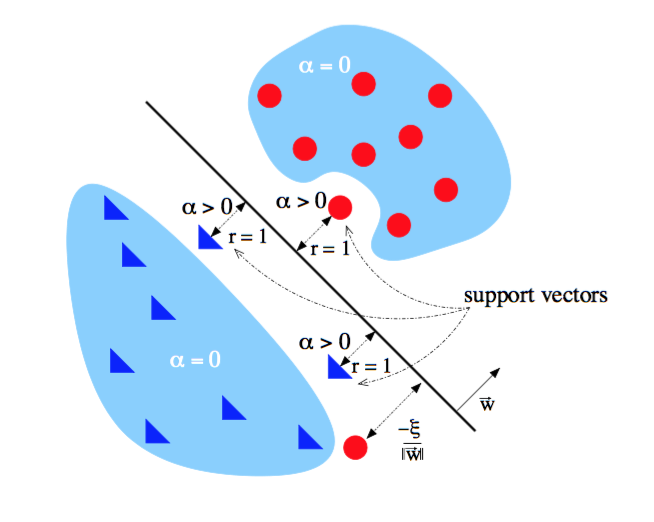
\includegraphics[width = 0.6\textwidth]{./notes/immagini/l13-non-linear.png}
\caption{SVM con dati non linearmente separabili.}
\end{figure}

L'idea è quindi quella di andare a sommare alla funzione costo la sommatoria di tutti i $\xi_i$ dei vari esempi presenti nel training set, moltiplicata per un coefficiente di penalizzazione \textit{C} che rappresenta un iper-parametro dell'algoritmo di apprendimento, da ottimizzare con le tecniche di model selection.

La nuova formula da minimizzare diventa:

$$ \frac{1}{2}||\vec{w}||^2 + C \sum\limits_{i=1}^n \xi_i $$

In pratica vengono penalizzati (aumentato il costo) gli esempi che non rispettano il margine.

La minimizzazione avviene considerano il problema duale, che risulta essere definito come:

$$max_\alpha \sum\limits_{i=1}^n \alpha_i - \frac{1}{2}\sum\limits_{i,j = 1}^n y_i y_j \alpha_i \alpha_j (\vec{x}_i \cdot \vec{x}_j)$$

$$ \text{s.t.: } \forall i \in \{1, \ldots, n\} : 0 \leq \alpha_i \leq C \text{ e } \sum\limits_{i=1}^n y_i \alpha_i = 0$$

Da notare che le $\xi_i$ sono variabili del problema primale e che quindi non compaiono nel problema duale.

Questa strategia per esempi non linearmente separabili non sempre
garantisce buone prestazioni perché un iper-piano può solo rappresentare
dicotomie dello spazio delle istanze.

Per questo motivo, quando gli esempi non sono linearmente separabili su
usa una strategia divisa in due passi:

\begin{enumerate}
\item
  Si mappano i dati di ingresso (input space) in uno spazio a dimensione
  molto superiore (feature space). Quindi a partire dalle feature degli
  elementi dell'input space vengono creati nuovi esempi nel feature
  space che utilizza combinazioni non lineari delle feature del primo
  spazio.
\item
  Si calcola poi l'iper-piano ottimo per il nuovo spazio usando la
  formulazione precedente (che prende il nome di variabili slack).
\end{enumerate}

Perché dovrei farlo?

\begin{enumerate}
\item
  Perché il \textbf{teorema sulla separabilità di Cover} afferma che un problema di classificazione complesso, formulato
  attraverso una trasformazione non lineare dei dati in uno spazio ad
  alta dimensionalità, ha maggiore probabilità di essere linearmente
  separabile che in uno spazio a bassa dimensionalità.
\item
  Perché l'iper-piano ottimo minimizza la VC-Dimension e quindi la
  capacità di generalizzazione migliora.
\end{enumerate}

Viene quindi utilizzata una trasformazione $\varphi(\cdot)$ non lineare, da applicare ai dati originari del problema $\{(\vec{x}_i, y_i)\}_1^n$ tale che:

$$ \forall i \: \vec{x}_i \in R^m, \varphi(\vec{x}_i) = \vec{Z}, \vec{Z} \in R^M, M \gg m $$

Il vettore ottenuto può essere rappresentato come $\vec{\varphi}(\vec{x}) = [ \varphi_1(\vec{x}), \ldots , \varphi_M(\vec{x}) ] $.

Con questa notazione è possibile andare a definire l'iper-piano nel nuovo spazio con:

$$ \sum\limits_{j=1}^M w_j \varphi_j(\vec{x}) + b = 0$$

che se si considera il termine noto $b = w_0$ e si aggiunge $\varphi_0(\vec{x}) = 1$, risulta essere

$$ \sum\limits_{j=0}^M w_j \varphi_j(\vec{x}) = \vec{w} \cdot \vec{\varphi}(\vec{x}) = 0$$

Andando a sostituire il $\vec{w}$ dell'equazione precedente con $ \vec{w} = \sum\limits_{k=1}^n j_k \alpha_k \vec{\varphi}(\vec{x}_k)$ si ottiene:

$$ \sum\limits_{k=1}^n j_k \alpha_k \varphi(\vec{x_k}) \cdot \varphi(\vec{x}) = 0 $$

Con il termine $\varphi(\vec{x}_k) \cdot \varphi(\vec{x})$ rappresenta il prodotto scalare tra un vettore del training set $\vec{x}_k$ e il vettore in input $\vec{x}$ calcolato nello spazio $R^M$.

\subsection{Funzioni Kernel}\label{funzioni-kernel}

Lo spazio di dimensione superiore serve solo per calcolare il prodotto scalare tra i due vettori, si può quindi definire una funzione $K(\cdot, \cdot)$ che prende il nome di kernel e che calcola il prodotto scalare dei due vettori senza passare esplicitamente nello spazio di dimensione superiore.

$$ K(\vec{x}_k, \vec{x}) = \varphi(\vec{x}_k) \cdot \varphi(\vec{x})$$

Assumendo di avere una di queste funzioni, l'iper-piano risulta essere:

$$\sum\limits_{k=1}^n  y_k \alpha_k K(\vec{x}_k, \vec{x}) = 0$$

Per il teorema di Mercer esistono delle funzioni di questo tipo, ma è necessario che soddisfino determinate condizioni.

Alcune di queste sono:

\begin{itemize}
\item \textbf{Polinomiale di grado \textit{p}}: $K(\vec{x},\vec{y}) = (\vec{x} \cdot \vec{y} +1) ^p$
\item \textbf{RBF}: $ K(\vec{x},\vec{y}) = exp(-\frac{1}{2\sigma^2}||\vec{x}-\vec{y}||^2)$
\end{itemize}

La formulazione duale del problema risulta quindi essere:

$$max_\alpha \sum\limits_{i=1}^n \alpha_i - \frac{1}{2}\sum\limits_{i,j = 1}^n y_i y_j \alpha_i \alpha_j K(\vec{x}_i ,\vec{x}_j)$$

$$ \text{s.t.: } \forall i \in \{1, \ldots, n\} : 0 \leq \alpha_i \leq C \text{ e } \sum\limits_{i=1}^n y_i \alpha_i = 0$$

Per fare la classificazione viene utilizzato il \textbf{segno} della funzione:

\begin{align*}
f(\vec{u})  &= \sum\limits_{i = 1}^n y_i  \alpha_i  K(\vec{x}_i,  \vec{u}) + b
\end{align*}

\subsection{Regressione}\label{regressione}

Quando si considera il problema di approssimazione di funzioni a valori
reali (regressione) si utilizza l'$\epsilon$-tubo: output che differiscono dai
valori di target per più di $\epsilon$ in valore assoluto vengono penalizzati
linearmente, altrimenti non vengono considerati errori. In pratica
aggiungo un intervallo di tolleranza al iper-piano che partiziona lo
spazio.

\begin{figure}[htbp]
\centering
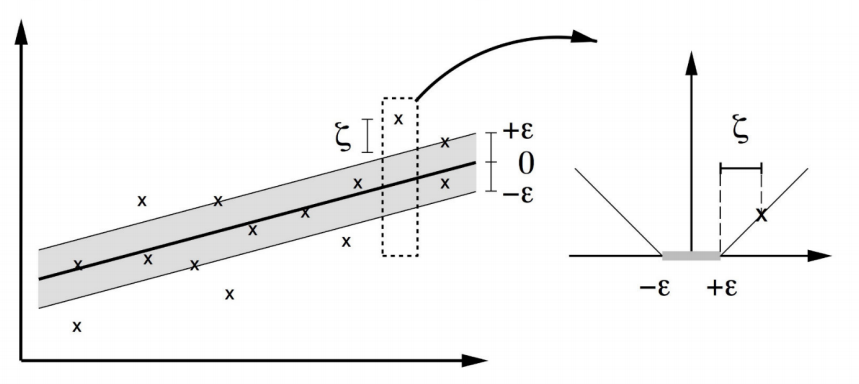
\includegraphics[width = 0.8\textwidth]{./notes/immagini/l13-primale-duale.png}
\caption{Regressione in forma primale (a sinistra) e duale (a destra)}
\end{figure}

\todo[inline]{Mancano formule (ultime due slide) http://www.math.unipd.it/\~{}aiolli/corsi/1516/aa/SVM.pdf}
	% !TEX encoding = UTF-8
% !TEX program = pdflatex
% !TEX root = MEMOC.tex
% !TEX spellcheck = it-IT

% 15 Dicembre 2016

\todo[inline]{Da recuperare}
	\section{Lezione 15 - Apprendimento Bayesiano}\label{lezione-15---apprendimento-bayesiano}

Si tratta di algoritmi di apprendimento basati sulla probabilità e sul
teorema di Bayes che effettuano la classificazione utilizzando l'ipotesi che
più probabilmente approssima la funzione target, scegliendola da un'insieme di funzioni $H$.

\subsection{Scelta delle ipotesi}\label{scelta-delle-ipotesi}

Tutto si basa sulla formula di Bayes.

$$
P(h | D) = \frac{P(D|h)P(h)}{P(D)}
$$

Dove:

\begin{itemize}
\item $P(h)$ è la probabilità a priori che l'ipotesi \textit{h} sia corretta e rispecchia la conoscenza a priori che si ha sul dominio;
\item $P(D)$ è la probabilità a priori che vengano osservati i dati \textit{D};
\item $P(h|D)$ è la probabilità che l'ipotesi \textit{h} sia corretta per i dati \textit{D};
\item $P(D|h)$ è la probabilità che i dati \textit{D} vengano classificati correttamente da \textit{h} \end{itemize}

L'obiettivo è quello di massimizzare \emph{P(h\textbar{}D)}, sapendo
\emph{P(D\textbar{}h)} che viene fornito dal supervisore e \emph{P(h)}
che viene appresa.

Nel massimizzare si può tralasciare il termine \emph{P(D)} dal momento
che è sempre costante.

$$
h_{MAP} = argmax_{h \in H} P(D|h)P(h)
$$

$H_{MAP}$ prende il nome di \textbf{ipotesi massima a posteriori}.

Si può inoltre assumere che tutte le ipotesi \emph{h} abbiano la stessa probabilità a priori, e nel mondo reale questa assunzione è tipicamente corretta, il
problema di massimizzazione diventa:

$$
h_{ML} = argmax_{h \in H} P(D|h)
$$

In questo caso si sceglie l'ipotesi di \textbf{maximum likelihood}

A pagina 158 del Mitchel c'è un esempio che mette in evidenza come le
probabilità a priori influenzino il risultato.

\subsection{Brute Force MAP Learning (interpretazione Find-S)}\label{brute-force-map-learning-interpretazione-find-s}

L'apprendimento dell'ipotesi massima avviene adattando l'algoritmo Find-S per l'apprendimento di concetti.

Si assumono fissate le istanze $x_1, \ldots, x_n$ e \textit{D} essere l'insieme dei valori desiderati $D = \{ c(x_1), \ldots, c(x_n)\}$.

Considerando inoltre tutte le ipotesi equiprobabili: $P(h) = \frac{1}{|H|}$, si ha che:

$$
P(D|h) = 
	\begin{cases}
		1,& \text{ se \textit{h} è consistente con \textit{D}} \\
		0,& \text{ altrimenti }
	\end{cases}
$$

L'algoritmo di apprendimento risulta quindi essere:

\begin{enumerate}
\item Per ogni potesi $h \in H$ calcola $P(h|D)$;
\item Scegli l'ipotesi che massimizza $P(h|D)$.
\end{enumerate}

Se i dati di apprendimento sono senza rumore e se la funzione target è contenuta nello spazio delle ipotesi \textit{H}, è possibile calcolare \emph{P(h\textbar{}D)} applicando la regola di Bayes, in particolare:

$$
P(h|D) = 
	\begin{cases}
		\frac{1}{|VS_{H,D}|},& \text{ se \textit{h} è consistente con \textit{D}} \\
		0,& \text{ altrimenti }
	\end{cases}
$$

Quindi se tutte le ipotesi \emph{h} sono equiprobabili, allora qualsiasi
ipotesi presente in \emph{H} va bene con probabilità $\frac{1}{VS_{H,D}}$, dove $VS_{H,D}$ è un sottoinsieme di \textit{H} consistente con \textit{D}.

Con questa definizione, tutte le ipotesi consistenti hanno probabilità $\frac{1}{VS_{H,D}}$ e tutte quelle non consistenti hanno probabilità \textit{0}, pertanto tutte le ipotesi consistenti possono essere delle $h_{MAP}$.

Segue anche che l'algoritmo Find-S ritorna sempre $h_{MAP}$ anche se non vengono utilizzate esplicitamente le probabilità.

Se vengono cambiate le probabilità in modo che la probabilità di
un'ipotesi più specifica sia più alta si ottiene che
\emph{P(h\textbar{}D) = P(h)}.

\subsection{Apprendimento di una funzione (ML)}\label{apprendimento-di-una-funzione-ml}

Si vuole apprendere una funzione $f$ a valori reali, utilizzando come esempi di apprendimento $(x_i, d_i)$ dove il valore target $d_i$ può contenere del rumore:

$$
d_i = f(x_i) + e_i
$$

dove $e_i$ è l'errore che segue una probabilità gaussiana con media 0 di
cui non si conosce la varianza.

Però si vuole valutare l'errore come se al posto di \emph{f} (che è sconosciuta) ci fosse \emph{h}

$$
e_i = d_i - h(x_i)
$$

La probabilità di $P(d_i | h)$, cioè che l'ipotesi \emph{h}
classifichi correttamente $d_i$ segue la distribuzione guassiana di
$e_i$.

Dalla definzione di ipotesi \textit{maximum likelihood} si ottiene che l'ipotesi $h_{ML}$ è anche quella che minimizza il quadrato degli errori:

\begin{align*}
h_{ML} &= argmax_{h \in H} P(D|h) \\
				&=  argmax_{h \in H} \prod\limits_{i=1}^m P(d_i|h) \\
				&= *\textit{gauassia di } e_i \textit{, logaritmi e altra math-magic*}\\
				&= arg min_{h \in H} \sum\limits_{i = 1}^m (d_i - h(x_i))^2
\end{align*}

Quindi per trovare l'ipotesi \textbf{maximum likelihood} è necessario
minimizzare l'errore quadratico, sotto l'ipotesi che la probabilità di
ogni ipotesi è uniforme e assumendo che i dati di apprendimento $d_i$ contengano del rumore che segue la distribuzione guassiana con media 0.

L'ipotesi \textit{MAP} coincide con l'ipotesi \textit{ML} solo se tutte le ipotesi hanno probabilità uniforme.

C'è anche da tenere in considerazione che questo approccio assume del rumore solamente nei dati $d_i$ e non dei vari $x_i$.

\subsection{Ipotesi MDL}

La scelta di questa ipotesi segue il principio del rasoio di Occam:``\textit{scegli la spiegazione più semplice per i dati osservati}'', ovvero sceglie l'ipotesi:

$$
h_{MDL} = argmin_{h \in H} L_{C_1}(h) + L_{C_2}(D|H)
$$

dove $L_C(x)$ è la lunghezza della descrizione di \textit{x} nella codifica \textit{C}.

Ad esempio, sfruttando la teoria dell'informazione è possibile utilizzare:

\begin{itemize}
\item $L_{C_1}(h) = - log_2(P(h))$
\item $L_{C_2}(D|h) = - log_2(P(D|h))$
\end{itemize}

Con questa codifica si ottiene che

\begin{align*}
h_{MDL} 	&= argmin_{h \in H} L_{C_1}(h) + L_{C_2}(D|H) \\
				&= argmin_{h \in H} - log_2(P(h)) - log_2(P(D|h)) \\
				&= argmax_{h \in H} P(D|h)P(h) \\
				&= h_{MAP}
\end{align*}

Ovvero che \textit{MDL} coincide con \textit{MAP}.

L'idea alla base di questo approccio è quella di effettuare un trade-off tra la complessità dell'ipotesi e il numero di errori commessi. L'ipotesi \textit{MDL} commette più errori sui dati di apprendimento a causa della sua brevità, ma ciò può essere visto come una limitazione dell'overfitting.

\subsection{Classificazione}\label{classificazione}

Finora abbiamo cercato l'ipotesi più probabile per i dati \emph{D}
($h_{MAP}$), ma dato un nuovo esempio, qual'è la classificazione più
probabile? Non sempre l'idea migliore è quella di calcolare $h_{MAP}(x)$.

Supponiamo di avere 3 ipotesi tali che: \emph{P($h_1$\textbar{}D)=0.4},\emph{P($h_2$\textbar{}D)=0.3},
\emph{P($h_3$\textbar{}D)=0.3} e che data una nuova istanza \emph{x} può si ottiene \emph{$h_1$(x) = (+)} e \emph{$h_2$(x) = $h_3$(x) = (-)}. 

In questo caso $h_{MAP}$, ovvero $h_1$, fornisce come classificazione $(+)$, anche se la classificazione più probabile è $(-)$.

Il \textbf{classificatore ottimo di Bayes} si basa su questo principio e classifica una nuova istanza $x$ con l'etichetta:

$$
v_x = argmax_{v_j \in V} \sum\limits_{h_i \in H} P(v_j | h_i)P(h_i | D)
$$

Dove:

\begin{enumerate}
\item $V$ è l'insieme di tutte le possibili classi
\item $
P(v_j | h_i) = 
	\begin{cases}
		1,& \text{ se } h_i(x) = v_j \\
		0,& \text{ altrimenti }
	\end{cases}
$
\end{enumerate}

Utilizzando lo stesso spazio delle ipotesi e la stessa conoscenza a priori, nessun altro classificatore riesce a superare il classificatore ottimo di Bayes.

Tuttavia, ad ogni classificazione è necessario calcolare la classificazione effettuata da ogni ipotesi $h_i$ e questo può essere computazionalmente oneroso al crescere del numero di ipotesi.

\subsection{Classificatore di Gibbs}\label{classificazione-di-gibbs}

Un'alternativa sub-ottima al classificatore di Bayes è data dall'algoritmo di Gibbs:

\begin{enumerate}
\item Sceglie un'ipotesi $h$ a caso, secondo $P(h|D)$,
\item utilizza l'ipotesi scelta per classificare l'istanza.
\end{enumerate}

Il classificatore così ottenuto è semplice da calcolare e funziona sorprendentemente bene dal momento che l'errore medio che compie è minore del doppio dell'errore effettuato dal classificatore ottimo:

$$
E[errore_{Gibbs}] \leq 2E[errore_{BayesOttimo}]
$$

Sempre assumendo probabilità a priori uniforme per tutte le ipotesi del version space.
	\subsubsection{Calcolabilità della minimalizzazione}\label{calcolabitliuxe0-della-minimalizzazione}

Se $ f : \mathbb{N}^{k+1} \rightarrow \mathbb{N} $ è in $ \mathcal{C} $, allora anche
$\mu y.f(\vec{x},y)$ è in $ \mathcal{C} $.

\paragraph{Dimostrazione}\label{dimostrazione}

Sia  $ f : \mathbb{N}^{k+1} \rightarrow \mathbb{N} $ in $ \mathcal{C} $ e sia \textit{P} il programma in
forma normale che calcola \textit{f}.

L'idea è quella di eseguire \emph{P} incrementando via via un contatore e, quando viene trovato un valore del contatore che azzera la funzione, questo viene ritornato.

\begin{verbatim}
 1       k         m+1          m+k|m+k+1|m+k+2|
|\vec{x} | .....  |x_1|x_2|....|x_k|  0  |  0  |
\end{verbatim}

Sia $m = \max{\rho(P), k }$, il programma che calcola la minimalizzazione illimitata è:

\begin{lstlisting}[language=URM]
T([1..k], [m+1..m+k]) //Copio l'input
P[m+1, ..., m+k+1 -> 1]
J(1, m+k+2, END) #LOOP
S(m+k+1)
J(1,1,LOOP)
#END
\end{lstlisting}

Dal momento che è possibile trovare un programma che calcola la
minimalizzazione illimitata, questa è calcolabile.

\subsubsection{Hot-fix delle funzioni} \label{hotfix}
Data una funzione  $ f : \mathbb{N} \rightarrow \mathbb{N} $ tale che esiste  $ g : \mathbb{N} \rightarrow \mathbb{N} $ calcolabile e tale che

$$
\Delta = \{ x | f(x) \neq g(x) \}
$$

e finito.

Allora \emph{f} è calcolabile e può essere modificata in modo da
coincidere con \emph{g}.

\subsubsection{Funzioni finite}\label{funizioni-finite}

\textbf{Funzione finita} $ \Theta: \mathbb{N}^{k} \rightarrow \mathbb{N}  $è una funzione
finita quando è definita come:

$$
\Theta(\vec{x}) = \begin{cases}
y_1, &\text{ se } \vec{x} = \vec{x}_1 \\
y_2, &\text{ se } \vec{x} = \vec{x}_2 \\ 
\cdots \\
y_n, &\text{ se } \vec{x} = \vec{x}_n \\
\uparrow, &\text{ altrimenti}
\end{cases}
$$

Tutte le funzioni di questo tipo sono calcolabili

\paragraph{Dimostrazione}\label{dimostrazione-1}

(per semplicità è ridotta a funzione unarie)

\begin{align*}
\Theta &= \begin{cases}
y_1, &\text{ se } x = x_1 \\
y_2, &\text{ se } x = x_2 \\ 
\cdots \\
y_n, &\text{ se } x = x_n \\
\uparrow, &\text{ altrimenti}
\end{cases} \\
&= y_1 \cdot \overline{sg}(|x - x_1|) + \cdots + y_n \cdot \overline{sg}(|x - x_n|) +  \underbrace{\mu z.\prod\limits_{i=1}^{n}|x - x_i|}_{\text{funzione indipendente da } z}
\end{align*}

La minimalizzazione su \emph{z} è calcolabile ma risulta indefinita, perché non è possibile minimizzarla rispetto a \emph{z}, quindi anche la funzione $ \Theta $ risulta essere indefinita se tutti i valori sono diversi da $ x_1 \ldots x_n $.

\section{Tesi di Church}\label{tesi-di-church}

Ogni funzione è calcolabile tramite un procedimento effettivo se e solo
se è URM calcolabile.

Church non ha proprio detto questo, perché non c'era URM quando è stata
enunciata e ha utilizzato un modello alternativo: le funzioni parziali
ricorsive $ \mathcal{R} $ (G\"{o}edel).

La classe $ \mathcal{R} $ delle \textbf{funzioni parziali ricorsive} è la \textbf{minima} classe di funzioni che contiene:

\begin{enumerate}[(a)]
\item  zero: $ z(\vec{x}) = 0 $ per ogni \textit{x}
\item  successore: $ S(x) = x+1 $
\item  proiezioni: $ U_{i}^k (x_1 \ldots x_k) = x_i $
\end{enumerate}

ed è chiusa rispetto:

\begin{enumerate}
\item
  composizione generalizzata
\item
  ricorsione primitiva
\item
  minimalizzazione illimitata.
\end{enumerate}

Una classe di funzioni \emph{X} è \textbf{ricca} se contiene le funzioni
di base ed è chiusa rispetto alle 3 operazioni classiche.

C'è almeno una classe ricca, perché anche la classe ``tutte le
funzioni'' è ricca, anche se ha poco senso considerarla.

Si vuole quindi che $ \mathcal{R} $ sia contenuta in \emph{X} ricca e che anche
$ \mathcal{R} $ sia ricca.

Questo è possibile perché l'intersezione di due classi ricche è
ovviamente anch'essa ricca.

$ \mathcal{R} $ può essere definita come l'intersezione di tutte le classi di
funzioni ricche.

$$
\mathcal{R} = \bigcap_{X \text{ ricca}} X
$$

anche se precedentemente $ \mathcal{R} $ è stata definita come

$$
\mathcal{R} = \{ (a), (b), (c) \text{ con tutte le funzioni che si ottengono da queste utilizzando } 1,2,3 \}
$$

È dimostrabile che le due definizioni sono equivalenti, anche se non lo
dimostriamo.

Si può anche definire la classe $ \mathcal{PR} $ delle \textbf{funzioni
primitive ricorsive}: la minima classe che contiene solamente le funzioni
di base chiusa rispetto la composizione e la ricorsione primitiva.
Ovviamente $ \mathcal{PR} $ è più piccola di $ \mathcal{R} $.

\subsection{$ \mathcal{C} $ = $ \mathcal{R} $}\label{c-figa-r-figa}

È già stato dimostrato che $ \mathcal{C} $ è una classe ricca, quindi sicuramente
$ \mathcal{R} \subseteq \mathcal{C} $.

Resta da dimostrare che $ \mathcal{C} \subseteq \mathcal{R} $.

Sia \textit{f} in $ \mathcal{C} $, ovvero esiste un programma \emph{P} in forma normale
che la calcola $f = f_p^{(k)}$.

\begin{verbatim}
P= I_1 ... I_s

|x_1 ... x_k| 0 ... 0
\end{verbatim}

Supponiamo di avere le funzioni:

$$
C_{p}^1(\vec{x},y) = \begin{cases}
\text{contenuto di R1 dopo \textit{t} passi del programma se non è terminato} \\
\text{altrimenti ritorna il valore finale del registro}
\end{cases} 
$$

$$
J_p(\vec{x},t) = \begin{cases}
\text{la prossima istruzione da eseguire all'istante \textit{t} di } P(\vec{x}) \text{ se non è terminato}\\
0 \text{ altrimenti }
\end{cases}
$$

Si ha che entrambe le funzioni sono del tipo $\mathbb{N}^{k+1} \rightarrow \mathbb{N} $
e totali.

Se $f(x)\downarrow$ allora \emph{P} termina su $\vec{x}$ in un qualche
numero di passi

$$
t_0 = \mu t.J_p(\vec{x}, t)
$$

e

$$
f(\vec{x}) = C_{p}^1(\vec{x}, t_0) =  C_{p}^1(\vec{x}, \mu t.J_p(\vec{x}, t))
$$

Se invece $f(\vec{x})\uparrow$ si ha che

$$
\mu t.J_p(\vec{x}, t) = \uparrow
$$

e

$$
f(\vec{x}) = C_{p}^1(\vec{x}, t_0) =  C_{p}^1(\vec{x}, \mu t.J_p(\vec{x}, t))
$$

Ovvero la combinazione di queste funzioni riesce a descrivere un programma URM.

Resta da dimostrare che queste due funzioni sono contenute in $ \mathcal{R} $ e pertanto, dato che \textit{f} è la combinazione di queste funzioni, anche \textit{f} è in $ \mathcal{R} $.

	% !TEX encoding = UTF-8
% !TEX program = pdflatex
% !TEX root = AALP.tex
% !TEX spellcheck = it-IT

Anche Java8 ha le clojure. Le variabili libere che vengono catturate devono essere dichiarate come final oppure non devono essere presenti tentativi di modificata dei dai (\textit{effectivly final}).
Java8 ha i method refernces, che permettono di usare dei metodi al posto delle lambda expression.


	% !TEX encoding = UTF-8
% !TEX program = pdflatex
% !TEX root = AALP.tex
% !TEX spellcheck = it-IT

\section{Lezione 18}

Con le \textbf{class extension} è possibile aggiungere al volo dei metodi ad una classe.

Una funzione o metodo che prende in input un valore di un tipo e lo utilizza per costruire un valore di un altro tipo, può essere visto come un convertitore di tipo. Un metodo di questo genere può essere marcato come \texttt{implicit}, in questo modo il compilatore, anziché non compilare una conversione di tipo, utilizza questo metodo per effettuarla.

Per effettuare una class extension è necessario definire una sotto-classe del tipo da estendere la quale definisce i nuovi metodi da aggiungere e anche un metodo \texttt{implict} per convertire il tipo originale nel tipo esteso.


Nel sub-classing c'è la necessità di specificare la keyword override. Questo aiuta a gestire il problema della classe base fragile, che si verifica quando vengono aggiunti dei metodi alle classi base della gerarchia.

I \textbf{traits} sono un'approssimazione di una classe astratta/interfaccia: possono contenere sia del codice concreto che del codice astratto e non possono essere istanziati.
Sta alle classi implementare (\textit{mix-in}) uno o più traits.

Un trait può estendere una classe \textit{A}, in questo caso il trait può essere mixato solamente con le sotto-classi di $A$.

I trait hanno binding dinamico sia su \texttt{this} che su \texttt{super}.

I mixin non sono commutativi, l'ordine con i quali li definiscono influisce sull'oggetto. L'ultimo trait che ho mixato è il primo ad essere eseguito.










	\subsection{Verifica delle false occorrenze}\label{verifica-delle-false-occorrenze}

Il metodo di Rabin-Karp può trovare delle false occorrenze anche se la probabilità che queste compaiano è molto bassa .

L'algoritmo di Mathukrishnan serve per verificare se ci sono o meno delle false occorrenze in tempo \emph{O(n)}.

L'algoritmo prende in input la lista delle posizioni in cui c'è un'occorrenza vera o meno e identifica una falsa occorrenza utilizzando la distanza tra queste due posizioni.

Siano $ pos_{i-1} $ e $ pos_{i} $ due occorrenze consecutive segnalate dall'algoritmo di Karp e sia $ d = pos_{i} - pos_{i-1}$ la distanza tra queste.

Se $ d \leq m/2 $\footnote{Perché una stringa sia periodica, questa deve avere un periodo $ 0 \leq 2d \leq m $.} ed entrambe sono occorrenze effettive, il pattern \textit{P} ha un bordo di lunghezza $ m -d $ e quindi $ d  $ è un periodo sia del pattern, che della stringa $ T[pos_{i-1}, pos_{i} +m -1] $.

Inoltre, se \textit{P} avesse anche un periodo proprio $ p < d $ la porzione di testo $ T[pos_{i-1}, pos_{i} +m -1] $ dovrebbe avere anche essa il periodo $ p $ e quindi dovrebbe esserci un'occorrenza del pattern anche a partire da $ pos_{i-1} + p$, ma siccome non c'è questa occorrenza, la stringa non può avere periodo $ p $, quindi $ d $ è il più piccolo periodo proprio di $ P $.

L'algoritmo suddivide quindi le possibili occorrenze in \textbf{corse}, ovvero una sequenza di possibili occorrenze tali che $ pos_{i} - pos_{i-1} \leq m/2  $.

Se la corsa è composta da una sola posizione, l'algoritmo verifica direttamente se c'è un'occorrenza del pattern, confrontando il pattern con la stringa.

Se invece la cosa contiene più elementi $ pos_s, pos_{s+1}, \ldots, pos_{t} $, l'algoritmo verifica direttamente le prime due occorrenze $pos_{s}$ e $ pos_{s+1} $, se c'è una falsa occorrenza l'algoritmo termina, altrimenti la distanza $ d = pos_{s} - pos_{s+1} $ è il più piccolo periodo del pattern \textit{P} e quindi se per qualche $ i = s+2, \ldots, t  $ si ha che $ pos_i - pos_{i-1} \neq d $, l'algoritmo termina segnalando una falsa occorrenza.

Questo è corretto perché se $ pos_i - pos_{i-1} < d $, $ d $ non sarebbe il periodo minimo mentre se $ pos_i - pos_{i-1} > d $, c'è una falsa occorrenza perché dovrebbe esserci anche un'occorrenza intermedia.

Se l'algoritmo trova che tutte le distanze sono uguali a $ d $ deve soltanto controllare che la parte $ T[pos_s +m, pos_t + m -1] $ abbia effettivamente periodo $ d $ e questo viene fatto in tempo proporzionale alla lunghezza, confrontando tra loro i caratteri.


\begin{breakablealgorithm}
\caption{\textsc{MathukrishnanTest}: verifica della presenza di false occorrenze}
\begin{algorithmic}[1]
\Function{MathukrishnanTest}{$P,T,pos,k$}
	\If{$ k = 0 $}
		\State \Return false
	\EndIf
	\State $ j \gets 1 $
	\While{$ P[j] = T[pos[1] + j -1] $}
		\State $ j \gets j+1 $
	\EndWhile
	\If{$ j \leq m $} \Comment{è una falsa occorrenza}
		\State \Return True
	\EndIf
	\State $ i \gets 2 $
	\While{$ i \leq k $}
		\State $ j \gets 1 $
		\While{$ P[j] = T[pos[i] + j -1] $}
			\State $ j \gets j+1 $
		\EndWhile
		\If{$ j \leq m $} \Comment{è una falsa occorrenza}
			\State \Return True
		\EndIf
		\If{$ pos[i] - pos[i-1] \leq m/2$}
			\State $ s \gets i -1 $
			\State $ p \gets pos[s+1] - pos[s] $
			\While{$ i+1 \leq k \textbf{ and  } pos[i+1] - pos[i] = p$}
				\State $ i \gets i+1 $
			\EndWhile
			\If{$ i+1 \leq k \textbf{ and  } pos[i+1] - pos[i] \neq p$}
				\State \Return True
			\EndIf
		\EndIf
		\For{$ j \gets pos[s] +m +p \textbf{ to } pos[i] +m -1 $}\Comment{tutte le posizioni della corsa sono a distanza corretta, controllo se la porzione di testo ha periodo $p $}
			\If{$ T[j] \neq T[j-p] $}
				\State \Return True
			\EndIf
		\EndFor
	\EndWhile
\EndFunction
\end{algorithmic}
\end{breakablealgorithm}

\subsubsection{Complessità}\label{complessituxe0}

Per ogni corsa si hanno al massimo $pos_t - pos_s - d$ caratteri da verificare, se il risultato è negativo viene segnalata una falsa occorrenza e l'algoritmo termina, altrimenti passa alla corsa successiva.

Durante la verifica di una corsa, ogni carattere del testo viene confrontato al massimo 2 volte con i caratteri del pattern più 1 volta con il carattere successivo del testo.

Dal momento che le corse distinte non si sovrappongono, si ha che vengono fatti al massimo \emph{O(3n)} confronti, che portano ad una complessità di \emph{O(n)}.

\section{Alberi dei suffissi}\label{alberi-dei-suffissi}

L'albero dei suffissi permette di evidenziare maggiormente la struttura interna di una stringa, permettendo così di risolvere in tempo lineare il pattern matching esatto, così come altri problemi di pattern matching più complesso.

Con il pattern matching esatto è possibile effettuare una pre-elaborazione del testo in \emph{O(n)} dopo la quale è possibile verificare in tempo \emph{O(m)} la presenza del pattern, rendendo questi algoritmi adatti ai problemi che hanno un testo fisso che deve essere matchato con più pattern distinti.

L'\textbf{albero dei suffissi} per una stringa \emph{S} di lunghezza \emph{n} è costituito da:

\begin{itemize}
\item  \emph{n} foglie numerate da 1 ad \emph{n}.
\item  Ogni nodo interno, eventualmente esclusa la radice, ha almeno due figli.
\item  Ogni arco è etichettato con una sottostringa di \emph{S}.
\item  Due archi uscenti dallo stesso nodo non possono avere etichette che iniziano con lo stesso carattere.
\item  La concatenazione delle etichette lungo il cammino dalla radice alla foglia etichettata \emph{i} è il suffisso $S[i,n]$ di lunghezza $ n-i+1 $
\end{itemize}

\begin{figure}[htbp]
\centering
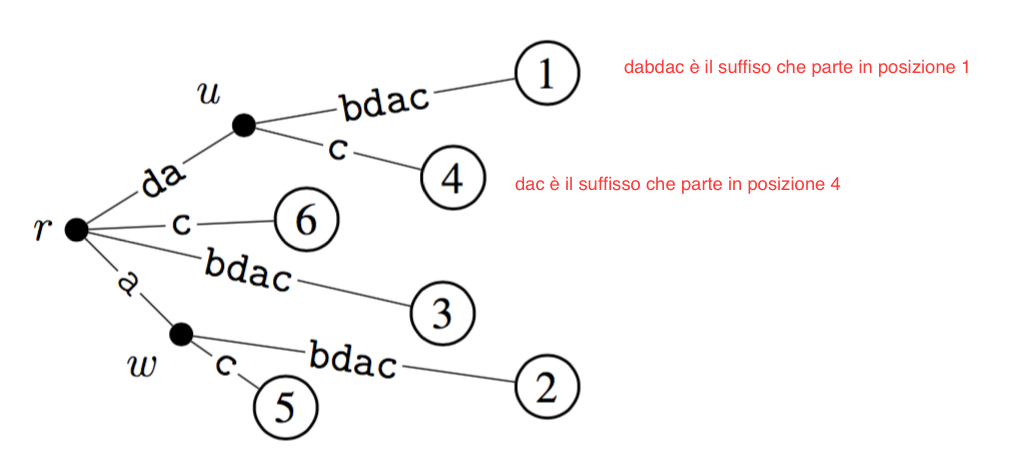
\includegraphics[width=.7\textwidth]{./notes/immagini/l19-fig1.png}
\caption{Albero dei suffissi della stringa $ S = dabdac $}
\end{figure}

Da notare che non sempre è possibile costruire l'albero dei suffusi, perché se un suffisso è anche prefisso di un altro suffisso, il cammino relativo a quel suffisso termina in un nodo interno dell'albero, violandone la definizione. 
Per evitare questo problema è necessario aggiungere un carattere sentinella alla fine della stringa. Assumeremo che questa ci sia sempre.

Nell'esempio \emph{S=dabdac} è \emph{c} che fa da sentinella, se non ci fosse non sarebbe possibile costruire l'albero.

L'\textbf{etichetta di un cammino} è la concatenazione delle etichette degli archi del cammino, mentre l'etichetta di un nodo \emph{u} è data dall'etichetta del cammino dalla radice al nodo.

Se l'etichetta di un arco $ (u,v) $ tra due nodi interni ha lunghezza \textit{k} maggiore di 1, l'arco è in realtà diviso in \textit{k} parti, una per ogni carattere dell'etichetta, mediante $ k-1 $ \textbf{nodi impliciti} le cui etichette sono la concatenazione dell'etichetta di \textit{u} con i caratteri dell'etichetta dell'arco $ (u,v) $ che precedono il nodo stesso.

\subsection{Matching esatto con l'albero dei suffissi}\label{matching-esatto-con-lalbero-dei-suffissi}

\begin{enumerate}
	\item Costruisci l'albero dei suffissi \textit{A} per il testo \textit{T}.
	\item Confronta i caratteri del pattern \textit{P} con i caratteri dell'unico cammino in \textit{A} individuato da essi. Questo cammino è unico perché tutti gli archi uscenti di un nodo sono associati a caratteri distinti. Seguendo questo cammino si possono verificare due casi:
	\begin{enumerate}
		\item Si esauriscono i caratteri del pattern e si passa al passo successivo
		\item Ci sono ancora dei caratteri del pattern ma non è possibile proseguire il cammino, in questo caso non ci sono occorrenze del pattern nel testo e l'algoritmo può terminare.
	\end{enumerate}
	\item Se si arriva alla fine del pattern, allora questo è uguale all'etichetta del nodo \textit{u} a cui si è arrivati, indipendentemente dal fatto che \textit{u} sia un nodo implicito o meno. Il pattern \textit{P} è quindi prefisso di tutti i suffissi associati alle foglie del sotto-albero radicato in \textit{u}. Le posizioni d'inizio di questi suffissi sono quindi tutte e sole le posizioni in cui \textit{P} occorre in \textit{T} e dal momento che queste posizioni sono memorizzate nelle foglie del sotto-albero, è sufficiente esplorarlo fino alle foglie per risalire alle posizioni di occorrenza del pattern.
\end{enumerate}

\subsubsection{Complessità del matching esatto}\label{complessituxe0-del-matching-esatto}

C'è una complessità \emph{O(n)} per la costruzione dell'albero (che per il momento non è stata vista).

Durante il secondo passo, per ogni carattere del pattern viene fatto
\begin{itemize}
	\item Un confronto se l'algoritmo sta analizzando un nodo implicito (c'è un solo arco uscente)
	\item Al più tanti confronti quanti sono i caratteri dell'alfabeto se è un nodo esplicito (al massimo ci sono tanti archi uscenti quanti sono i caratteri dell'alfabeto).
\end{itemize}

In ogni caso il numero di confronti è minore o uguale di una costante e quindi il passo 2 ha complessità $ O(m) $.

Il terzo passo richiede tempo proporzionale al numero di nodi del sotto-albero radicato in \textit{u}.
Se nel testo ci sono \textit{k} occorrenze del pattern, questo sotto-albero ha esattamente \textit{k} foglie e siccome ogni nodo interno ha almeno due archi uscenti, il numero di nodi interni è $ \leq k-1 $, quindi il terzo passo richiede $ O(k) $.

Siccome $ k \leq n $, il tempo totale richiesto è $ O(n+m) $, come per gli altri algoritmi, con la differenza che il carico di lavoro è sbilanciato verso la preelaborazione e non verso la ricerca (risulta più conveniente cercare più pattern nello stesso testo).

\subsection{L'algoritmo naive per la costruzione dell'albero} \label{lalgoritmo-naive-per-la-costruzione-dellalbero}

L'albero dei suffissi per la stringa $S[1,n]$ viene costruito a partire dal suffisso più lungo della stringa \textit{S}, ovvero tutta la stringa, per poi aggiungere gli altri suffissi $S[i,n]$ con $i = 2, \ldots, n+1$. 

Con $A_i$ viene indicato l'albero intermedio che contiene tutti i suffissi che iniziano nelle posizioni da 1 a \emph{i}.

L'albero $A_1$ contiene solamente un unico arco etichettato con $S[1,n]\$$ che congiunge la radice e il nodo \emph{1}.

Ogni albero $A_{i+1}$ viene costruito nel seguente modo:

\begin{enumerate}
	\item Partendo dalla radice di $ A_i $ viene cercato il più lungo cammino che raggiunge un nodo la cui etichetta è prefisso del suffisso $ S[i+1,n]\$ $ da aggiungere.
	
	Il cammino che si ottiene è unico in quanto ogni nodo implicito ha un solo arco uscente e tutti gli archi uscenti da uno stesso nodo esplicito sono associati a caratteri diversi.
	Inoltre, la ricerca deve terminare prima della fine del suffisso $ S[i+1,n]\$ $ perché la sentinella assicura che il suffisso non sia prefisso di nessuno dei prefissi più lunghi inseriti precedentemente nell'albero.
	
	\item Se il nodo in cui termina la ricerca è implicito, questo viene sostituito da un nodo esplicito, spezzando l'arco che lo contiene in due archi e l'etichetta in due etichette.
	
	\item A questo punto il nodo \textit{u} sul quale è terminata la ricerca è un nodo esplicito con etichetta $ S[i+1,j] $ tale che nell'albero non ci sia un nodo con etichetta $ S[i+1,j+1] $ e quindi tutti gli archi uscenti hanno etichette che iniziano con un carattere diverso da $ S[j+1] $.
	
	Viene quindi aggiunto un nuovo arco uscente da \textit{u} a $ i+1 $ con etichetta $ S[j+1,n]\$ $ che congiunge \textit{u} con la foglia numerata $ i+1 $.
	
	A questo punto l'albero ottenuto contiene un unico cammino dalla radice alla foglia $ i+1 $ la cui etichetta è il suffisso $ S[i+1,n]\$ $, ovvero l'albero ottenuto è $ A_{i+1} $
\end{enumerate}

\subsubsection{Complessità dell'algoritmo}\label{complessituxe0-dellalgoritmo}

Quando devo aggiungere un suffisso vengono passati al più tutti caratteri del suffisso e non appena viene trovato un carattere diverso, vengono aggiunti tanti nodi quanti sono i caratteri del suffisso restanti, ottenendo così una complessità $ O(n) $.
Dal momento che una stringa di lunghezza \textit{n} ha \textit{n} suffissi distinti, la complessità totale dell'algoritmo è $ O(n^2) $, dove $ n^2 $ è moltiplicato per una costante pari alla cardinalità dell'alfabeto.

\subsection{Algoritmo di Ukkonen}\label{algoritmo-di-ukkonen}

Questo algoritmo costruisce l'albero dei suffissi un carattere alla volta, partendo dall'inizio della stringa.

Così facendo viene persa la condizione che un suffisso non possa essere un prefisso dell'albero, per questo si dice che l'algoritmo crea una successione di \textbf{alberi dei suffissi impliciti}.

Un albero dei suffissi implicito è un albero simile a quello normale, con la differenza che viene rimossa la condizione che il cammino relativo ad ogni suffisso della stringa \textit{S} termini in una foglia e viene preso in considerazione anche il suffisso nullo.

\begin{figure}[htbp]
	\centering
	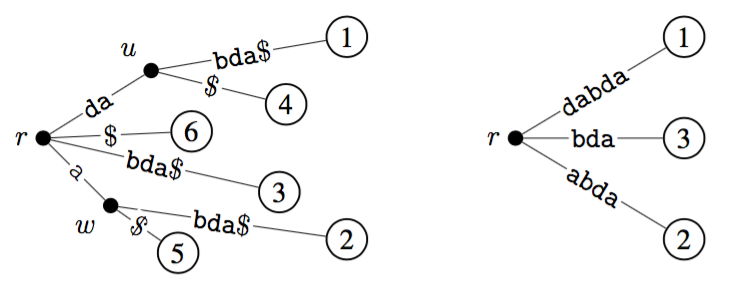
\includegraphics[width=.7\textwidth]{./notes/immagini/l19-fig2.png}
	\caption{Albero dei suffissi normale e implicito per la stringa $ S = dabda $.}
\end{figure}

L'algoritmo di Ukkonen costruisce un albero dei suffissi implicito $ I_i $ per ogni prefisso $ S[1,i] $ della stringa $ S\$ $ di lunghezza $ n+1 $ e incrementando \textit{i} finché non arriva a costruire $ I_{n+1} $. Siccome $ S[1,n+1] = S\$ $, l'albero dei suffissi implicito $ I_{n+1} $ coincide con l'albero dei suffissi \textit{A}, perché nessun suffisso della strina $ S\$ $ è prefisso di un altro suffisso.

\begin{breakablealgorithm}
	\caption{Ukkonen: Descrizione generale dell'algoritmo }
	\begin{algorithmic}[1]
		\Function{Ukkonen}{$S$}
			\State $ S \gets S\$ $ \Comment{Aggiunge la sentinella a $ S $}
			\State ``Costruisci $ I_0 $ ''
			\For{$ i = 0 \textbf{ to } n $}
				\For{$ j = 1 \textbf{ to } i+1 $}
					\State ``Cerca la fine del cammino relativo al suffisso $ S[j,i] $ in $ I_i $''
					\State ``Se necessario estendi il cammino con il carattere $S[i+1] $ in modo che il suffisso $ S[j,i] $ diventi un suffisso di $ S[1,i+1] $''
				\EndFor
			\EndFor
		\EndFunction
	\end{algorithmic}
\end{breakablealgorithm}

La costruzione di $ I_0 $ è banale in quanto contiene solo la radice e nessun arco uscente, perché la stringa $ S[1,0] $ ha come suffisso solamente $ \epsilon $.

Per costruire $ I_{i+1} $ è necessario modificare tutti i suffissi $ S[j,i] $ di $ S[1,i] $ nei suffissi $ S[j,i+1] $ di $ S[1,i+1] $.
Durante questa modifica possono verificarsi 3 casi:

\begin{enumerate}
	\item Il cammino etichettato $ S[j,i] $ termina in una foglia numerata $ j $. In questo caso il nuovo carattere $ S[i+1] $ viene aggiunto all'etichetta dell'ultimo arco del cammino (viene messo un nuovo nodo implicito).
	\item Il cammino etichettato $ S[j,i] $ termina in nodo interno \textit{u}, ma nessun cammino che parte da \textit{u} inizia con $ S[i+1] $. In questo caso viene creata una foglia etichettata $ j $ connessa al nodo \textit{u} con un arco etichettato $ S[i+1] $. Se \textit{u} è un nodo implicito, viene sostituito con un nodo esplicito, spezzando l'arco esistente.
	\item Il cammino etichettato $ S[j,i] $ termina in nodo interno \textit{u} e almeno un cammino che parte da \textit{u} è etichettato con $ S[i+1] $. In questo caso il suffisso $ S[j,i+1] $ è già presente nell'albero e non occorre fare niente.
\end{enumerate}

Dopo aver esteso tutti i suffissi di $ S[1,i] $ l'albero contiene tutti i suffissi di $ S[1,i+1] $, compreso il suffisso nullo che è sempre rappresentato.

\begin{figure}[htbp]
	\centering
	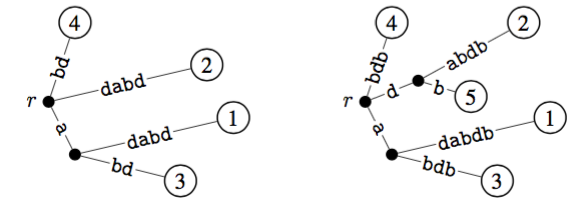
\includegraphics[width=.7\textwidth]{./notes/immagini/l19-fig3.png}
	\caption{Estensione dell'albero dei suffissi implicito per la stringa $ adabd $ quando si aggiunge alla stringa il carattere $ b $. I primi 4 suffissi vengono estesi con il caso 1, il quinto viene esteso con il caso 2 e il suffisso nullo viene esteso per il caso 3.}
\end{figure}

Tuttavia con questa implementazione si riesce a calcolare in $ O(i^2) $ l'albero $ I_{i+1} $ a partire da $ I_i $, portando ad una complessità totale di $ O(n^3) $ che è peggiore di quella dell'algoritmo naive.

	% gli esercizi sono finiti in separata sede
	\appendix
	% Recap 
	% !TEX encoding = UTF-8
% !TEX program = pdflatex
% !TEX root = AALP.tex
% !TEX spellcheck = it-IT
\chapter{Cose utili per l'orale}

\section{Lemmi vari}

\begin{itemize}
	\item \textbf{Lemma di Inversione}: mi dice che se riesco a tipare un termine con una certa regola di tipo, allora anche i vari sotto-termini sono ben tipati.
	\item \textbf{Lemma delle Forme Canoniche}: collega il tipo di un termine ai possibili valori per quel tipo.
\end{itemize}

\section{Teoremi notevoli}

\begin{itemize}
	\item \textbf{Teorema di Progressione}: se $M$ è un termine chiuso e ben tipato($\emptyset \vdash M :T $), allora $M$ è un valore oppure $\exists M'$ tale che $M \to M'$. Si dimostra per induzione sulla derivazione del giudizio di tipo.
	\item \textbf{Teorema di Preservazione (subject-reduction)}: Se $M$ è un termine ben tipato ($\Gamma \vdash M :T $) e $M \to M'$, allora anche $M'$ è ben tipato con tipo $T$ ($\Gamma \vdash M' : T$). Si dimostra per induzione sulla derivazione del giudizio di tipo, oppure sulla derivazione $M \to M'$.
	\item \textbf{Corollario di Preservazione} Se $\emptyset \vdash M : T$ e $M \to^* M'$, allora $\emptyset M':T$.
	\item \textbf{Teorema di Safety}: Se $M$ è un termine chiuso e ben tipato, $M \to M'$ con $M' \not\to$, allora $M'$ è un valore.
\end{itemize}

\section{Dimostrazione per induzione sulla struttura dei termini}

\begin{itemize}
	\item \textbf{Casi base}: li definisco per i termini che non hanno sotto-termini. Ad esempio se devo dimostrare che l'esecuzione di un programma è deterministica, i casi base dimostrano che i valori del linguaggi, che sono i termini senza sotto-termini, non possono ridursi ulteriormente e quindi per loro il teorema è banalmente provato.
	\item \textbf{Casi induttivi}: per ogni possibile termine del linguaggio ragiono sulla sua struttura, sfruttando l'ipotesi induttiva sui sotto-termini del termine in esame. Continuando con il precedente esempio: se $M = A + B$, prima osservo quali regole di riduzione posso applicare e poi nell'applicarle uso l'ipotesi induttiva, perché sfruttando il fatto che l'evoluzione dei sotto-termini ($A \to A'$) di $M$ è deterministica. Ottengo quindi che, dato che posso applicare solo una regola alla volta, l'esecuzione rimane deterministica.
\end{itemize}

\section{Dimostrazione per induzione sulla derivazione $\Gamma \vdash M : T$}

\begin{itemize}
	\item \textbf{Casi base}: dimostro il teorema su tutti gli assiomi del sistema di typing. Ad esempio per dimostrare i casi base del Teorema di Preservazione, parto dagli assiomi di tipi, i quali sono relativi ai valori del linguaggio e osservo che in quel caso il teorema è valido perché i valori non possono essere ridotti ulteriormente.
	\item \textbf{Casi induttivi}: dimostro il teorema per tutte le regole di tipo del sistema di typing, sfruttando il fatto che i sotto-alberi che partono dalla derivazione del giudizio sono di altezza inferiore e quindi posso applicare l'ipotesi induttiva. Ad esempio, per il caso relativo alla regola di tipo \myrule{Sum} nella dimostrazione di Preservazione so che il termine $M$ ha tipo $\Nat$ e che i due sotto-termini hanno tipo $\Nat$ (perché $M$ è ben tipato). Osservo poi che il termine può evolvere con 3 possibili regole: \myrule{Sum}, \myrule{SumLeft} e \myrule{SumRight}. Prendiamo per esempio il caso \myrule{SumLeft} e quindi $M' = A' + B$. So già che $B : \Nat$ perché compare in $M$, mentre per $A'$ posso sfruttare l'ipotesi induttiva, perché $A \to A'$ e $\Gamma \vdash A : \Nat$ è una derivazione più corta rispetto a quella di partenza. Quindi anche $A' : \Nat$ e pertanto posso ottenere che $M'$ è di tipo $\Nat$ applicando la regola \myrule{Sum}. 
\end{itemize}

\section{Dimostrazione per induzione sulla riduzione $M\to M'$}

\begin{itemize}
	\item \textbf{Casi base}: sono quelli in cui la riduzione $M \to M'$ avviene per effetto di un assioma. Devo quindi dimostrare il teorema per ogni assioma della SOS.
	
	Ad esempio nella dimostrazione del teorema di Preservazione, nel caso base \myrule{Sum} ho $M = n_1 + n_2$ e che $M$ è ben tipato con tipo $T$. In primo luogo applico il lemma di inversione per ottenere che $T = \Nat$. 
	Inoltre, $M' \equiv n$ per effetto della regola semantica \myrule{Sum} e sempre per il lemma di Inversione $M'$ ha tipo $\Nat$. Segue quindi che $M\to M'$ e $M'$ ha lo stesso tipo di $M$, ovvero il teorema di Preservazione è valido anche per questo caso.
	
	\item \textbf{Casi induttivi}: sono quelli in cui la riduzione $M \to M'$ avviene per effetto di una regola della SOS. Devo quindi dimostrare il teorema per ognuna di queste regole.
	
	Ad esempio nella dimostrazione del teorema di Preservazione, nel caso induttivo \myrule{SumLeft}, ho che $M = A + B$ e che $M$ è ben tipato. Per il Lemma di Inversione $M$ deve essere di tipo $\Nat$ e lo stesso vale per i suoi sotto-termini $A$ e $B$. 
	Per effetto della regola \myrule{SumLeft} ho che $M' = A' +B$ con $A \to A'$.
	Dato che la derivazione $A \to A'$ richiede meno passi, posso assumere che sia valida l'ipotesi induttiva e che quindi anche $A'$ abbia tipo $\Nat$.
	Posso quindi tipare $M'$ con la regola di tipo \myrule{Sum} e quindi anche $M'$ è di tipo $\Nat$.
	Segue quindi che $M$ e $M'$ hanno lo stesso tipo e pertanto è provato il teorema di preservazione.
\end{itemize}












	% Formulario
	
\section{Appello 2015-07-16}

\subsection{Esercizio 1 - Teorema di proiezione}

$$
P(x,\vec{y}) \text{ semi-dedibile} \Rightarrow \exists x \: P(x,\vec{y}) \text{ semi-decidibile}
$$

\subsubsection{Soluzione}

Per il teorema di struttura: $P(\vec{x})$ è semi-decidibile $\Leftrightarrow$ esiste un predicato $Q(\vec{x}, y)$ tale che $P(\vec{x}) \equiv \exists y \: Q(\vec{x}, y)$.

Quindi essendo $P(x,\vec{y})$ è semi-decidibile, per il teorema di struttura esiste $Q(x, \vec{y}, z)$ decidibile.

Si può quindi riscrivere $P'$ come:

$$
P'(\vec{y}) \equiv \exists x \: \exists z Q(x, \vec{y}, z) \equiv \exists w . Q( (w)_1, \vec{y}, (w)_2)
$$

con $Q$ decidibile e quindi per il teorema di struttura $P'(\vec{y})$ è semi-decidibile.

\subsection{Esercizio 2 - Teoria sulla riduzione}

$$
A \text{ è RE } \Leftrightarrow A \leq_m K
$$

\subsubsection{Soluzione}

\paragraph{$(\Rightarrow)$} 

Essendo $K$ RE, la sua funzione semi-caratteristica $SC_K(x)$ è calcolabile ed esiste per ipotesi una funzione di riduzione $f : \mathbb{N} \rightarrow \mathbb{N}$.

Si possono quindi combinare queste due funzioni per definire la funzione semi-caratteristica di $A$:

$$
SC_A(x) = SC_K(f(x))
$$ 

la quale risulta calcolabile e quindi $A$ è RE.

\paragraph{$(\Leftarrow)$}

Per ipotesi $A$ è RE, quindi la sua funzione semi-caratteristica è calcolabile.

Serve quindi una funzione di riduzione $f : \mathbb{N} \rightarrow \mathbb{N}$ per dimostrare che $A$ si riduce a $K$.

Vogliamo quindi trovare una funzione tale che se $x \in A$, allora $f(x) \in K$, ovvero $\phi_{f(x)}(x) = \downarrow$ e che se $x \notin A$ allora $f(x) \notin K$ e quindi $\phi_{f(x)}(x) = \uparrow $.

Possiamo quindi definire la funzione

$$
g(x,y) = \begin{cases}
1 &\text{se } x \in A \\
\uparrow &\text{altrimenti}
\end{cases} = SC_A(x)
$$

Questa funzione è calcolabile perché equivale alla funzione semi-caratteristica di $A$. 

Possiamo quindi utilizzare il teorema SMN per trovare una funzione calcolabile e totale che ritorni un programma che calcoli $g$:

$$
\phi_{f(x)}(y) = g(x,y)
$$ 

La funzione $f$ è quindi la funzione di riduzione cercata, perché:

\begin{itemize}
	\item $x \in A$: $\phi_{f(x)}(y)$ è $\downarrow \: \forall y$ ed in particolare $\phi_{f(x)}(x) \downarrow$ e quindi il programma $f(x) \in K$
	\item $x \notin A$: $\phi_{f(x)}(y)$ è sempre indefinita ed in particolare $\phi_{f(x)}(x) $ è indefinita e quindi $f(x) \notin K$.
\end{itemize}


\subsection{Esercizio 3 - Studio della ricorsività (riduzione)}

$$
A = \{ x \in \mathbb{N} \:|\: \exists y \in E_x, \exists z \in W_x, x = y \cdot z  \}
$$

\subsubsection{Soluzione}

L'insieme $A$ sembra essere RE perché per stabilire l'appartenenza ad $A$ di una determinato programma è necessario andare ad eseguirlo su un certo numero di valori, fino a che non viene trovata una coppia che soddisfa la condizione.

La funzione semi-caratteristica può quindi essere scritta come:

$$
SC_A(x) = 1 \bigg( \mu w . \Big( S\big(x, (w)_1, (w)_2, (w_3)\big) \wedge H\big(x, (w)_4, (w)_5\big) \wedge \big( x = (w)_2 \cdot (w)_4 \big)  \Big) \bigg)
$$

che risulta calcolabile e quindi $A$ è RE.

Il primo termine cerca un numero di passi $(w)_3$ entro i quali il programma $x$ produce un output $(w)_2 = y$ avendo in input $(w)_1$. In pratica prova vari valori di input per trovare i valori del dominio.

Il secondo termine cerca tutti i valori di input $(w)_4$ che fanno terminare il programma $x$ in meno di $(w)_5$ passi.

$A$ sembra inoltre essere non ricorsivo e questo può essere dimostrato riducendo $K \leq_m A$.

Si vuole quindi una funzione $f : \mathbb{N} \rightarrow \mathbb{N}$ tale che se $x \in K$, ovvero il programma $x$ termina quando riceve in input se stesso, produca un programma $f(x)$ tale che ci siano almeno un elemento del dominio e uno del codominio che possono essere tra loro moltiplicati per ottenere l'indice del programma. 

Viceversa se $x \notin K$, il programma $f(x)$ non deve avere questa coppia di valori nel dominio/codominio.

\textbf{Osservazione}: basta trovare un programma che termina producendo in output 1 quando in input riceve se stesso. In questo caso si ha che $1 \in E_x$ e che $x \in W_x$ e quindi la condizione di appartenenza ad $A$ è soddisfatta.

Si può quindi definire la funzione

$$
g(x,y) = \begin{cases}
1 &\text{se } x \in K\\
\uparrow &\text{altrimenti}
\end{cases} = SC_K(x)
$$

tale funzione è calcolabile e quindi per il teorema SMN esiste una funzione $f$ tale che $\phi_{f(x)}(y) = g(x,y)$.

Questa funzione è proprio quella di riduzione perché:

\begin{itemize}
	\item $x \in K$: $\phi_{f(x)}(f(x)) = 1$ e $f(x) \in W_{f(x)}$ e quindi $f(x) \in A$.
	\item $x \notin K$: $\phi_{f(x)}$ è sempre indefinita e quindi $E_{f(x)} = W_{f(x)} = \emptyset$, non è quindi possibile trovare $y$ e $z$ e pertanto $f(x) \notin A$.
\end{itemize}

Dal momento che $A$ è RE e non è ricorsivo, $\overline{A}$ non è RE.

\subsection{Esercizio 4 - Studio della ricorsività (Rice-Shapiro)}

\begin{align*}
	B &= \{ x \:| \: x \in \mathcal{B} \} \\
	\mathcal{B} &= \{ f \: |\: |dom(f) \setminus cod(f) | \geq 2 \}
\end{align*}

Ovvero $\mathcal{B}$ contiene tutte le funzioni che hanno il dominio con più di due elementi diversi dal codominio.

\subsubsection{Soluzione}

Dal momento che $\mathcal{B}$ descrive una proprietà (non banale) di una funzione, l'insieme è saturo e quindi di sicuro $B$ non è ricorsivo.

L'idea è quindi quella di applicare Rice-Shapiro per dimostrare che $B$ non è RE. Per fare questo si può trovare una funzione $f \notin \mathcal{B}$ ma che ha almeno un parte finita $\vartheta \in \mathcal{B}$.

$$
f(x) = x \dotminus 2 = \begin{cases}
0 &x \leq 2 \\
x -2 &\text{altrimenti}
\end{cases}
$$

In questo caso si ha $dom(f) = cod(f) = \mathbb{N}$, $| dom(f) \setminus cod(f)| = 0$ e quindi $f \notin \mathcal{B}$.

Come parte finita di $f$ si può considerare

$$
\vartheta(x) = \begin{cases}
0 & x \leq 2 \\
\uparrow &\text{altrimenti}
\end{cases}
$$

Si ha che $dom(\vartheta) = \{0,1,2\}$, $cod(f) = \{0\}$ e quindi $\vartheta \in \mathcal{B}$.

Abbiamo quindi una funzione $f \notin \mathcal{B}$ che ha una parte finita $\vartheta \subseteq f$ che appartiene a $\mathcal{B}$ e quindi per Rice-Shapiro $B$ non è RE.

Resta da valutare $\overline{\mathcal{B}} = \{ f \: | \: |dom(f) \setminus cod(f)| < 2 \}$, che può essere fatto allo stesso modo.

Basta osservare che la funzione $1 \notin \overline{\mathcal{B}}$  e che ha come parte finita la funzione $\emptyset \in \overline{\mathcal{B}}$ e quindi sempre per Rice-Shapiro $\overline{\mathcal{B}}$ non è RE.


\subsection{Esercizio 5 - Secondo teorema di ricorsione}

Dimostrare che 

$$
 \exists x . W_x = \{ kx \: | \: k \in \mathbb{N} \}
$$

\subsubsection{Soluzione}

Il secondo teorema di ricorsione afferma che data una funzione calcolabile e totale $h : \mathbb{N} \rightarrow \mathbb{N}$, esiste $e \in \mathbb{N}$ tale che $\phi_{h(e)} = \phi_e$.

Come prima cosa è necessario cercare una funzione che produca un programma $f(x)$ con le caratteristiche desiderate, ovvero che termini quando riceve un multiplo di se stesso in input.

Si può quindi definire la funzione

$$
g(x,y) = \begin{cases}
k &\text{se } y = kx \text{ per qualche }k \\
 \uparrow &\text{altrimenti}
\end{cases} = \mu k . |kx - y|
$$

Essendo $g$ calcolabile, per il teorema SMN, esiste una funzione $f : \mathbb{N} \rightarrow \mathbb{N}$ calcolabile e totale, tale che il programma $f(x)$ calcoli $\phi_{f(x)}(y) = g(x,y)$.

Si ha quindi che $W_{f(x)} =  \{ kx \: | \: k \in \mathbb{N} \}$, ma noi stiamo cercando un programma $e$.
	
Però la funzione $f$ soddisfa le condizioni del secondo teorema di ricorsione, quindi $\exists e \in \mathbb{N} \text{ tale che } \phi_e = \phi_{f(e)}$ e quindi si ha che

$$
W_e = W_{f(e)} =  \{ ke \: | \: k \in \mathbb{N} \}
$$
	
	
	
	%%\renewcommand{\glossaryname}{Glossario}

%\newglossaryentry{Cordova}
%{
%	name=\glslink{Cordova}{Cordova},
%	text=Cordova,
%	sort=Cordova,
%	description={Apache Cordova è un framework open source per la realizzazione di applicazioni ibride che offre delle API che permettono di accedere via JavaScript ad alcune funzionalità native del dispositivo, come l'accelerometro o la fotocamera}
%}
\subsection*{A}

\underline{\textbf{ARPA}}: %TODO

\underline{\textbf{ARPANET}}: %TODO

\underline{\textbf{Assembler}}: %TODO

\subsection*{B}

\underline{\textbf{Beowulf}}: %TODO

\subsection*{C}

\subsection*{D}

\underline{\textbf{Debian}}: %TODO

\underline{\textbf{DFSG}}: %TODO

\subsection*{E}

\subsection*{F}

\underline{\textbf{Free Software Foundation}}: %TODO

\underline{\textbf{Freeware}}: %TODO

\underline{\textbf{fsf}}: %TODO

\subsection*{G}

\underline{\textbf{GNU}}: %TODO

\underline{\textbf{GPL}}: %TODO

\subsection*{H}

\subsection*{I}

\subsection*{J}

\subsection*{K}

\underline{\textbf{Kernel}}: %TODO

\subsection*{L}

\underline{\textbf{Linux}}: %TODO

\subsection*{M}

\underline{\textbf{Mimix}}: %TODO

\underline{\textbf{MUTIX}}: %TODO

\subsection*{N}

\underline{\textbf{Netscape}}: %TODO

\underline{\textbf{nslu2}}: %TODO

\subsection*{O}

\underline{\textbf{OSI}}: %TODO

\subsection*{P}

\underline{\textbf{PDP}}: %TODO

\subsection*{Q}

\subsection*{R}

\underline{\textbf{RedHat Enterprise Linux}}: %TODO

\underline{\textbf{Routes}}: %TODO



\subsection*{S}

\underline{\textbf{StarOffice}}: %TODO

\underline{\textbf{Sun}}: 

\underline{\textbf{S\&P}}: %TODO

\underline{\textbf{Shareware}}: %TODO

\underline{\textbf{Symbolics}}: %TODO	

\subsection*{T}

\underline{\textbf{TECO}}: %TODO

\subsection*{U}

\underline{\textbf{Unix}}: %TODO

\subsection*{V}

\subsection*{W}

\subsection*{X}

\subsection*{Y}

\subsection*{Z}


	




	
	
\end{document}